\documentclass[a4paper, 12pt, oneside, spanish]{report}
\usepackage[T1]{fontenc}
\usepackage[utf8]{inputenc}
\usepackage{lmodern}
\usepackage{layout}
\usepackage{emptypage}
\usepackage{fancyhdr}
\usepackage[spanish,activeacute]{babel}
%\usepackage[Conny]{fncychap}
%\usepackage{graphicx}
\usepackage{subfigure} % subfiguras
\usepackage{caption}
\usepackage{mathtools}
\usepackage{hyperref}
\usepackage[a4paper,top=3cm, bottom=3cm, inner=2.5cm, outer=2.5cm]{geometry}
\usepackage{listings}
\usepackage[spanish]{babel}
\usepackage{url}
\usepackage{float}
\usepackage{multirow}
\usepackage{rotating} 
\usepackage{color}
\usepackage{colortbl}
\usepackage[table]{xcolor}
\usepackage{enumerate}
\usepackage{enumitem}
\usepackage{multicol}
\usepackage{mwe}
\usepackage[acronym, nonumberlist]{glossaries}
\makeglossaries

\makeatletter
\renewcommand{\@makeschapterhead}[1]{%
%  \vspace*{50\p@}%
  \vspace*{0\p@}%
  {\parindent \z@ \raggedright
    \normalfont
    \interlinepenalty\@M
    \Huge \bfseries  #1\par \nobreak
%    \vskip 40\p@
    \vskip 15\p@
  }}
\makeatother

\renewcommand{\baselinestretch}{1.4}
\setlength{\headheight}{16pt} 
\captionsetup{justification=justified}
\pretolerance=1000

\chead[]{}
\rhead[]{}
\renewcommand{\headrulewidth}{0.5pt}

\pagestyle{empty}

\title{Pr\'acticas Docentes de Rob\'otica en el Entorno JdeRobot-Academy}
\author{Pablo Moreno Vera}

\lstset{
	float=hbp,
	basicstyle=\ttfamily\small,
	columns=flexible,
	tabsize=4,
	frame=single,
	extendedchars=true,
	showspaces=false,
	showstringspaces=false,
	numbers=none,
	numberstyle=\tiny,
	breaklines=false,
	breakautoindent=true,
	captionpos=b
}
\setcounter{tocdepth}{4}
\setcounter{secnumdepth}{4}

\definecolor{lightgray}{gray}{0.9}

\begin{document}
%%%%%%%%%%%%%%% Portada %%%%%%%%%%%%%%%%%%%%
\begin{titlepage}
	\begin{center}
		\vspace*{3mm}
		\begin{center}
			
\includegraphics[width=0.8\linewidth]{figures/logo.jpg}
		\end{center}
		\vspace{6.5mm}
		
		\fontsize{15.5}{14}\selectfont ESCUELA TÉCNICA SUPERIOR DE INGENIERÍA DE TELECOMUNICACIÓN
		\vspace{13mm}
		
		\fontsize{14}{14}\selectfont DOBLE GRADO EN INGENIERÍA DE SISTEMAS \\ DE TELECOMUNICACIÓN Y ADMINISTRACIÓN Y DIRECCIÓN DE EMPRESAS
		
		\vspace{55pt}
		
		\fontfamily{lmss}\fontsize{15.7}{14}\selectfont \textbf{TRABAJO FIN DE GRADO} 
		
		\vspace{15mm}
		\begin{huge}
			Nuevas Prácticas Docentes de Robótica en el \\ \vspace{0.4cm} Entorno JdeRobot-Academy
		\end{huge}
		
		\vspace{15mm}
		
		\begin{large}
			Autor: Pablo Moreno Vera
			
			Tutor: José María Cañas Plaza
			
			\vspace{10mm}
		\end{large}
		\begin{normalsize}
			Curso académico 2018/2019		
		\end{normalsize}
		\vspace{10mm}
		
	\end{center}
	
\end{titlepage}

\pagenumbering{Roman}

%%%%%%%%%%%%%%% Agradecimientos %%%%%%%%%%%%
\newgeometry{top=1.6cm,left=2cm,right=2cm}
\chapter*{Agradecimientos}
\setlength{\parskip}{1ex}

Me gustaría aprovechar esta parte del trabajo para dar a conocer un poquito de mí, de mi esencia y qué la ha causado. Para dar a conocer por qué he conseguido llegar hasta donde estoy y por haber conseguido llegar siendo quién soy.

Quiero dar las gracias, en primer lugar, a mis padres, quienes nunca han dudado de mí, ni por un segundo. Me han apoyado en todo momento y me han llevado de la mano hasta donde estoy. Me han demostrado que hay que pelear cada paso, porque nadie te va a regalar nada y menos si es algo que merece la pena. Han conseguido sacar una sonrisa de los momentos más dolorosos y demostrarme que, a veces, sólo es necesario sonreír. Me han enseñado la importancia de la familia y sé que sin ellos no lo habría logrado. Hemos pasado malos momentos, de todo tipo, y hemos salido de ello juntos. Juntos hemos derrotado a una enfermedad que se lleva millones de vidas en el mundo y que, en muchas ocasiones, no tiene cura como es el cáncer y, aun teniendo que estudiar junto a la camilla de mi padre en el hospital hemos conseguido derrotarlo y aprobar mis asignaturas. Este título lo hemos conseguido los 3 juntos, gracias por todo.

También quiero dar las gracias a mi tutor José María, por mostrarme el camino hacia el éxito. Por enseñarme que sin esfuerzo y estudio no se alcanza ningún objetivo propuesto y por mostrarme la robótica. La ciencia que me ha mostrado un lugar de interés perpetuo, un campo en continuo desarrollo y en el cual, tras un año en el desarrollo de este Trabajo de Fin de Grado, sólo tengo conocimiento de una infinitésima parte. Te agradezco aquellas palabras de interés por mí al terminar tu examen para que decidiera unirme ti para que mostrases la robótica. Has hecho de mí una persona trabajadora y constante durante todas las semanas de reuniones contigo.

Quiero agradecer a mi familia los momentos de tranquilidad y locura que me aportáis. Sólo con aparecer hacéis que desconecte de todo y me dé cuenta de que no estoy solo, que tengo gente que me quiere a mi alrededor y no es fácil de encontrar en personas que no eliges, sino que forman parte de ti al nacer. Aun así, estaré siempre agradecido por pertenecer a ese pequeño sitio del mundo en el que estáis vosotros.

Gracias a mi pareja, Vida, por enseñarme que la felicidad puede estar en unos ojos. Por hacerme sonreír con una mirada y hacer que olvide todo lo que me rodea. Sin el descanso que me das no habría aguantado la presión y no lo habría conseguido. Me has ayudado con asignaturas de las que ni siquiera comprendías lo que te contaba y, aun así, sin ti no habría llegado aquí. Eres mi lugar de descanso al que acudir cuando todo lo demás tiembla.

Me gustaría dar las gracias a todas las personas que habéis aportado un poquito en mi vida, que habéis conseguido hacer de mí una persona que está escribiendo un Trabajo de Fin de Grado para terminar una carrera de 4 años en la que muchos no confiaban pudiese finalizar. Muchas gracias a ti, Gabriel, por enseñarme que hay personas que te acompañan por el camino y no te abandonan. A todos vosotros, gracias.

La última mención es para las personas que me han guiado desde las estrellas todos los días de mi vida, que me dan su amor desde el cielo y que me han visto convertirme en quién soy. Gracias a mis abuelos que me cuidan a cada paso que doy y que, aunque no puedan decirme cómo se sienten al verme, me dan fuerzas para enfrentarme a cualquier dificultad que he encontrado y que me encontraré durante el camino que me queda por recorrer hasta verlos de nuevo. Y sobre todo a ti abuela que, aunque el Alzheimer haya apartado tu consciencia de mí y el azar se haya llevado tu vista, sé perfectamente que tu alma ya está con el abuelo y con ella puedes verme y darte cuenta lo mucho que os echo de menos.

Gracias a todos.
\restoregeometry


%%%%%%%%%%%%%%% Resumen %%%%%%%%%%%%%%%%%%%%
\chapter*{Resumen}
\setlength{\parskip}{1ex}

Debido al auge de la robótica en la actualidad, cada vez encontramos productos desarrollados mediante la robótica a nuestro alrededor. Por ello se acrecenta la necesidad de especialistas en este campo. Es por esto que surgen plataformas y entornos dedicados a llevar el campo de la robótica a estudiantes de distintas edades. En claro ejemplo es el JdeRobot-Academy, el cual pne a disposición de los alumnos universitarios y pre-universitarios un conjunto de ejercicios que representan un problema específico de la robótica, de una manera sencilla, completa y eficaz.

Este Trabajo de Fin de Grado se ha centrado en el desarrollo de una nueva práctica para el entorno de JdeRobot-Academy, así como una completa reestructuración y optimización de una de las prácticas ya presente en el entorno. Para cada práctica se ha desarrollado una solución de referencia.

Para la nueva práctica incluida, llamada \textit{Chrono}, ha sido necesario el completo desarrollo del nodo académico, así como su interfaz gráfica, la conexión de sensores y actuadores del robot con el nodo académico y la sincronización del simulador con las grabaciones procedentes de \textit{ROS-Kinetic} para la visualización del robot F1 a vencer.
Esta práctica permite al alumno enfrentarse al problema de captación y procesado de imágenes, además de preparar un algoritmo de control de movimiento del robot.

Para la optimización y mejora de la práctica llamada \textit{Follow Road}, fue necesario una reestructuración de su interfaz gráfica para introducir una visualización de la imagen procesada por el alumno y la integración de una pausa académica, así como el desarrollo de un algoritmo nuevo de conexión de sensores y actuadores para dar soporte a los \textit{drivers} proporcionados por \textit{ROS-Kinetic}.
Para esta práctica se ponen a disposición del alumnos todos los materiales para que pueda centrarse exclusivamente en los problemas de captación y procesado de imágenes y de la realización de un movimiento controlado por parte del dron para que siag de una manera eficiente la carretera.
\cleardoublepage

%%%%%%%%%%%%%%% Ìndices %%%%%%%%%%%%%%%%%%%%
%\cleardoublepage
%\renewcommand{\tablename}{Tabla}
%\renewcommand{\listtablename}{\'Indice de tablas}
%\tableofcontents

%\cleardoublepage % ͭndice de figuras
%\addcontentsline{toc}{chapter}{\listfigurename}
%\listoffigures

%\cleardoublepage % ͭndice de tablas
%\addcontentsline{toc}{chapter}{\'Indice de tablas}
%\listoftables 
\cleardoublepage
\tableofcontents % indice de contenidos
\listoffigures % indice de figuras
\addcontentsline{toc}{chapter}{\'Indice de figuras} % para que aparezca en el indice de contenidos

\cleardoublepage

%%%%%%%%%%%%%%% Acronimos %%%%%%%%%%%%%%%%%%%%
%\include{0-Acronimos}

%%%%%%%%%%%%%%% Cap��tulos %%%%%%%%%%%%%%%%%%
\pagestyle{fancy}
\pagenumbering{arabic}
\setlength{\parindent}{6mm}

\lhead[]{CAP\'ITULO \thechapter. INTRODUCCI\'ON}
\chapter{Introducción}\label{cap.introduccion}
El Trabajo Fin de Grado (TFG) descrito a continuación pertenece a un entorno educativo para la enseñanza de la programación de robots. En este capítulo se desarrollará el contexto en el que se sitúa este proyecto y la motivación que he llevado a su desarrollo. Es preciso comenzar con una explicación a grandes rasgos sobre qué es la robótica y sus aplicaciones en la sociedad.

La parte funcional más importante en la robótica viene suministrada por el software. Dentro del software podemos destacar diferentes elementos como los simuladores, las bibliotecas de código y los middlewares de robótica, los cuales serán descritos en la segunda sección del capítulo. En la tercera sección de este capítulo se describirá la situación actual de la robótica en el panorama educativo y en el entorno de JdeRobot-Academy, en el cual está desarrollado este TFG. La intención principal de su desarrollo es extender este entorno docente con nuevos ejercicios que representen un problema en la robótica. En cuanto al desarrollo de un sistema robótico, hay numerosas cuestiones a las que enfrentarse y solucionar. A la mayoría de estos problemas se enfrenta y soluciona el entorno docente y se oculta al estudiante, para que se pueda centrar en los algoritmos que dotarán vida al robot.

\section{Robótica}
A lo largo de la historia, la ciencia y la tecnología han sido utilizadas por el hombre para facilitarle la vida. Para ello, ha ideado, desarrollado y construido herramientas y máquinas empleándolas para reducir su carga de trabajo. En este entorno se desarrolla la robótica, que es la rama de la tecnología basada en la utilización de la informática para el diseño y desarrollo de sistemas automáticos que faciliten la vida al ser humano e, incluso, llegar a sustituirle en algunas tareas determinadas. La robótica incluye conceptos de disciplinas diversas, como la física, las matemáticas, la electrónica, la mecánica, la inteligencia artificial, la ingeniería de control, etc. Gracias a todas estas disciplinas involucradas unidas convenientemente se pueden diseñas máquinas que ejecuten comportamientos autónomos según el propósito para el que han sido desarrolladas. Estas máquinas autónomas se denominan "Robots".

El término "Robot" fue concebido por Isaac Asimov en 1950. Desde entonces estos sistemas autónomos han experimentado un crecimiento exponencial en cuanto a complejidad, versatilidad, autonomía y, sobre todo, en su incorporación a una gran diversidad de ámbitos. Los sistemas operados por el ser humano comienzan a incorporar un sistema de control específico programable que permiten el desarrollo de tareas repetitivas o con un gran riesgo para las personas, englobando tareas básicas y de difícil realización, hasta la actualidad, en la cual existe un gran marco de ejemplos en los que se integran la robótica y multitud de campos y tareas. Los robots comerciales e industriales realizan las tareas de una manera más exacta o más barata que las personas. También son utilizados en trabajos peligrosos, sucios tediosos para el ser humano. Gracias a esto, se trata de un campo en crecimiento constante.

\begin{figure}[H]
	\begin{center}
		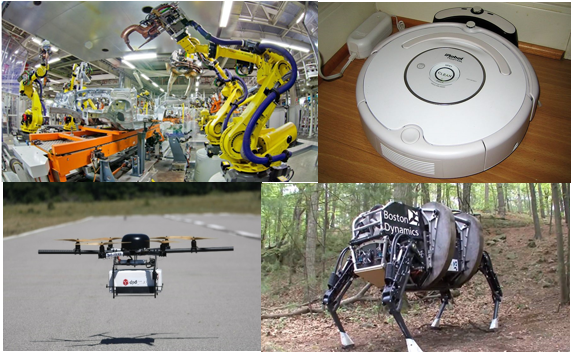
\includegraphics[width=0.8\textwidth]{figures/robots.png}
		\caption{Robots modernos}
		\label{fig.robots}
	\end{center}
\end{figure}

Ya se ha comentado la importancia de los robots en la actualidad en el aspecto industrial, pero tal el crecimiento que está experimentando la robótica que está comenzando a cobrar una gran importancia en aspectos menos especializados como el entorno doméstico. Cabe destacar el desarrollo de robots para facilitar la vida al ser humano, un ejemplo está ilustrado en la Figura 1.1. Las aspiradoras robóticas (Roomba, Dyson, Xiami, ...) han tenido un éxito rotundo en la realización de una actividad doméstica necesaria para la vida del ser humano. Otro éxito de la robótica en la actualidad es el desarrollo de coches autónomos. Este hecho se ha conseguido paulatinamente mediante la incorporación de tecnología cada vez más sofisticada a los automóviles. En este aspecto cabe destacar los módulos de aparcamiento automático, el park assist o los asistentes de conducción autónoma (autopiloto Tesla), o los prototipos de coches autónomos (Apple o Google). Otro ámbito en el que la robótica ha sido introducida es el militar, donde se han incorporado robots de rescate o para la desactivación de bombas. En la medicina se ha desarrollado el robot DaVinci, que permite operar desde cualquier parte del mundo con una precisión mayor a la humana. En el ámbito de la logística Amazon ha desarrollado una flota de robots de almacén que consiguen trasladar los pedidos a lo largo de sus almacenes. Tal es el punto de crecimiento de la robótica que se están desarrollando robots con "comportamientos inteligentes" como el robot Asimo de Honda (Figura 1.2) que pueden interactuar con humanos, ya sea como asistente para el hombre o con fines experimentales como la locomoción bípeda.

\begin{figure}[h]
	\centering
	\begin{minipage}[h]{.48\linewidth}
		\centering
		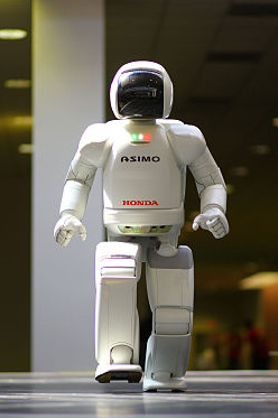
\includegraphics[width=.5\linewidth, height=7cm]{figures/asimo.png}
		\captionof{figure}{Robot Ásimo}
		\label{fig:asimo}
	\end{minipage}
	\begin{minipage}[h]{.48\linewidth}
		\centering
		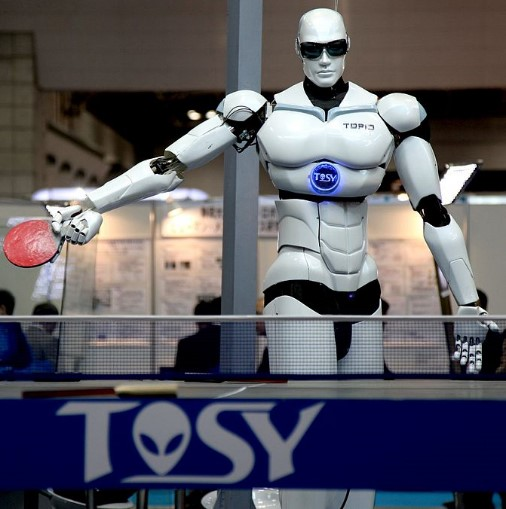
\includegraphics[width=.7\linewidth, height=7cm]{figures/topio.jpg}
		\captionof{figure}{Robot TOPIO}
		\label{fig:topio}
	\end{minipage}
\end{figure}

Los ámbitos en los que se puede aplicar la robótica es tan extenso como la imaginación de las personas dedicas a su creación, gracias a esto ámbitos en los que sólo podríamos imaginar automatizadas ahora son operadas totalmente con robots con resultados superiores a los de cualquier humano, como la agricultura de precisión mediante drones con análisis de imágenes térmicas y multiespectral para aumentar el rendimiento de las explotaciones agrícolas o el control de los productos industriales mediante el procesado de imágenes de la producción o la automatización de aplicaciones anestésicas de bajo nivel e, incluso, competiciones deportivas de robots.

Debido al gran potencial que tiene esta rama de la ciencia cobra una gran importancia la necesidad de dominarla. Gracias a ella ganaremos en comodidad, economía e, incluso, saludo. Es importante advertir de la importancia de la robótica en el futuro, ya que será la llave que abrirá la puerta a la humanidad hacia un mundo más seguro y sencillo mediante la automatización.

\section{Software Robótico}
Para que los robots puedan ser controlados de una manera eficaz el comportamiento del software que los controla debe ser robusto. Para ello se divide en distintas capas (\textit{drivers}, \textit{middleware} y aplicaciones), cuya arquitectura será distinta según su aplicación final.

Debido al gran desarrollo de la robótica, los robots actuales ya no precisan del control del ser humano para su funcionamiento, en la actualidad tienen comportamientos autónomos que les permiten realizar las tareas sin la mediación de terceros. Esto es posible gracias al minucioso desarrollo del software que compone los sistemas complejos del robot, algo parecido a una inteligencia autónoma. El desarrollo del software robótico parte de ciertas tareas o requisitos como son los circuitos de retroalimentación, control, búsqueda de caminos, localización o filtrado de datos entre otras muchas.

En los últimos años se han creado una gran cantidad de plataformas de desarrollo de software para las aplicaciones robóticas, también llamados /textit{middleware} robóticos. Los simuladores son otra parte importante para el desarrollo de software robótico ya que permiten realizar pruebas y depurar los fallos para programar una versión funcional del robot antes de ser fabricado. Esto supone un gran ahorro en costes. Estos componentes son vitales para generar el conjunto de comandos que componen la funcionalidad del robot, por ello entraremos en detalle en el siguiente apartado. Por último, las bibliotecas son necesarias para guardar los comandos que componen el funcionamiento del robot.

\subsection{Middlewares robóticos}
Los \textit{middleware} robóticos pueden definirse como entornos o \textit{frameworks} para el desarrollo de software pare robots. Se trata de software que conecta aplicaciones o componentes software para soportar aplicaciones complejas y distribuidas. Para controlar los sensores y actuadores de los robots estos entornos incluyen \textit{drivers}, arquitectura software para las aplicaciones que se van a crear, bloques de funcionalidad robótica ya resuelta, además de simuladores, visualizadores... Por ello al \textit{middleware} se le suele conocer como "pegamento para software". Una de las tareas del \textit{middleware} es conectar el hardware, ya sea real o simulado, con la aplicación desarrollada. El \textit{middleware} más extendido en el mundo es ROS.

	\textbf{Robot Operating System (ROS)\footnote{\url{http://www.ros.org/}}}

Se trata de una plataforma de software libre para el desarrollo software de robots que proporciona la funcionalidad de un sistema operativo en un clúster heterogéneo como el control de dispositivos de bajo nivel, mecanismos de intercambio de mensajes entre procesos y la abstracción del hardware, necesarios para el desarrollo de la robótica. Aunque el \textit{framework} ROS se desarrolló para los sistemas UNIX, se ha adaptado para ser soportado en otros sistemas operativos como Fedora, Debian, Windows, Mac OS X, Arch, Slackware, Gento u OpenSUSE, llegando a permitir las aplicaciones multiplataforma. Gracias a esto el \textit{framework} ROS se ha convertido en el más utilizado.

Existen otros \textit{framework} interesantes como:

	\textbf{Orocos}\footnote{\url{http://www.orocos.org/}}

Permitiendo el control avanzado de máquinas y robots en C++.

	\textbf{Orca}\footnote{\url{http://orca-robotics.sourceforge.net//}}

Está orientado a componentes por lo que permite el desarrollo de aplicaciones más complejas. Se tratta de un proyecto de software libre.

	\textbf{Urbi}\footnote{\url{https://github.com/urbiforge/urbi}}

Es un \textit{middleware} multiplataforma de código abierto en C++ que permite desarrollar aplicaciones en sistemas completos y complejos. Trabaja de forma conjunta con ROS.

	\textbf{JdeRobot}\footnote{\url{https://jderobot.org/}}

Plataforma de desarrollo de apicaciones robóticas y de visión artificial que incluye nodos programados con varios lenguajes de programación (Python o C++) compatible con \textit{middleware} de comunicaciones como ICE o ROS.

\subsection{Simuladores robóticos}
Debido al gran coste que supone la fabricación del hardware del robot es preciso depurar los posibles errores que contenga el código, así como el funcionamiento del hardware antes de su fabricación. Por ello debe probarse el código en un simulador orientado al tipo de aplicación que estemos desarrollando. Gracias a los simuladores es posible probar este código sin tener que fabricar previamente el hardware. De esta manera cualquier mal funcionamiento del código del robot puede ser solventado evitando la rotura del hardware. Algunos de los simuladores más utilizados son:

	\textbf{Gazebo}\footnote{\url{http://gazebosim.org/}}

Se trata del simulador 3D de código abierto más extendido. Funciona bajo la licencia Apache 2.0 y tienen gran importancia su motor de renderizado avanzado, sus motores de física y su soporte para \textit{plugins} de robot y sensores, además de su amplio catálogo de robots con sus sensores y actuadores. Otro hecho importante es su soporte para ROS lo que permite probar el código real del robot n el simulador.

	\textbf{Stage}\footnote{\url{http://wiki.ros.org/stage}}

Es un simulador en dos dimensiones, integrable con ROS, que permite simular numerosos robots simultáneamente.

	\textbf{Webots}\footnote{\url{https://www.cyberbotics.com/}}

Simulador de róbotica avanzada en el que se pueden desarrollar modelos propios y su física, escribir sus conroladores y hacer simulaciones a gran velocidad. Un ejemplo es su soporte para el humanoide Nao.

\subsection{Diseñadores Gráficos}
A la hora de introducir los modelos de los robots desarrollados en el simulador, así como un mundo simulado para comprobar la adaptación del mismo al medio, es necesario el uso de software de diseño gráfico. Este software permite la creación del modelo del robot e introducirla en el simulador. Gracias a esto se pueden ahorrar una gran cantidad de costes a la hora de desarrollar robots debido a que cualquier fallo estructural puede ser solventado antes incluso de la fabricación del prototipo. Algunos de los diseñadores gráficos más utilizados son:

	\textbf{SketchUp}\footnote{\url{https://www.sketchup.com/}}

Se trata de un programa de diseño gráfico y modelado en tres dimensiones basado en caras. Su principal característica es la realización de diseños en 3D de manera sencilla. Además incluye una extensa galería llamada 3D Warehouse que incluye esquemas de objetos, texturas e imágenes descargables. Este sofware de diseño es multiplataforma y de pago.

	\textbf{Blender}\footnote{\url{https://www.blender.org/}}

Es una programa de diseño gráfico dedicado especialmente al modelado, iluminación, renderizado, animación y creación de gráficos tridimensionales. También dispone de composición digital utilizand la técnica procesal de nodos, edición de vídeo, escultura (incluyendo topología dinámica) y pintura digital. También puede utilizarse para desarrollo de videojuegos dado que consta de una motor de juegos interno. Inicialmente fue distribuido de manera gratuita pero sin el código fuente, con un manual de uso, aunque posteriormente pasó a ser de software libre. Blender es multiplataforma con soporte para GNU/Linux, Windows, Mac OS X, Android, Solaris, FreeBSD e IRIX.

\subsection{Bibliotecas}
En el desarrollo de software deben abordarse un gran abanico de problemas clásicas, básicas y específicas para cada aplicación. Esta tarea es muy tediosa si hay que abordarla desde cero y requeriría un gran tiempo enfrentarse a ellas. Para evitar la repetición de problemas a la hora de desarrollar una aplicación, existen bibliotecas de código. Estas bibliotecas ofrecen conjuntos de implementaciones de código que permiten solucionar de manera directa ciertos problemas contenidos en su código. Esto permite al programador ahorrar una gran cantidad de tiempo para solucionar problemas que ya han sido solucionados anteriormente. Las bibliotecas pueden vincularse a un programa o a otra biblioteca en distintos puntos del desarrollo (bibliotecas estáticas) o durante la ejecución del programa (bibliotecas dinámicas). Algunas bibliotecas utilizadas en robótica son:

	\textbf{OpenCV}\footnote{\url{http://opencv.org/}}

Se trata de una biblioteca de código abierto que aborda problemas de visión artificial. Originalmente fue desarrollada por Intel y escrita en C++. En la actualidad contiene de interfaces en C++, Python, Java y MATLAB, además dispone de más de quinientas funciones que abarcan áreas de la visión artificial como reconocimiento de objetos y facial, calibración de cámaras y visión robótica y estéreo. Open CV es multiplataforma  y existen versiones para GNU/Linux, Mac OS X, Windows y Android.

	\textbf{OpenCV}\footnote{\url{http://pointclouds.org/}}

Es una librería utilizada para el procesamiento digital de imágenes RGBD mediante el tratamiento de nubes de puntos 3D. Entre sus numerosos algoritmos de última generación, se tratan problemas como filtrado, reconstrucción de superficies, ajuste de modelos, segmentación y estimación de características. Para simplificar el desarrollo, PCL se divide en bibliotecas de código  más pequeñas que pueden ser compiladas por separado. También es multiplataforma con soporte para Linux, Mac OS X, Windows y Android.

\section{Docencia en robótica}
La robótica con fines educativos está adquiriendo una gran importancia en la actualidad en la enseñanza preuniversitaria. Esto es debido a que su aprendizaje está disponible para estudiantes de cualquier nivel, el único requisito para estudiar robótico es la motivación por el desarrollo de aplicaciones. La robótica en el campo de la docencia cobra una gran importancia al ser una ciencia multidisciplinar, ya que incluye campos multidisciplinares como electrónica, informática, mecánica, física, ... Gracias a ello el estudiante adquiere una gran variedad de conocimiento de todas estas áreas. Además, proporciona una nueva visión del universo que le rodea, aprendiendo a distinguir los problemas y tomar una decisión al respecto.
En docencia primaria y secundaria se intenta despertar el interés del estudiante por la robótica, con la transformación de asignaturas teóricas tradicionales en asignaturas más prácticas e interactivas, ya que la robótica permite la recreación de problemas que les rodean y a través de los cuales pueden utilizar su creatividad y plasmar los conceptos teóricos que han adquirido.
En los centros de enseñanza primaria y secundaria se imparte robótica mediante plataformas físicas como los robots LEGO (Mindstorms, RCX, NXT, Evo, WeDo), placas Arduino, los kits de SolidWorks, etc.

\subsection{Docencias en la universidad}
En la docencia universitaria se imparte la robótica en distinto Grados y Postgrados en las escuelas de ingeniería. En España, se puede cursar la docencia robótica en el "Grado en Ingeniería Robótica" de la Universidad de Alicante, en los Grados de "Electrónica industrial y automática" o "Ingeniería Electrónica, Robótica y Mecatrónica" en distintas universidades, además de grados que están en desarrollo como el "Grado en Ingeniería Robótica Software" que imparte la Universidad Rey Juan Carlos desde el mes de Septiembre. Sin embargo, la docencia en robótica se reserva, mayoritariamente, para los Postgrados, dado que se trata una ciencia muy especializada. Existen varios Másteres destacados en cuanto a la docencia de robótica como el "Máster de Visión Artificial", el "Máster Universitario en Ingeniería Mecatrónica", o el "Máster Universitario en Automática y Robótica".
Dentro del ámbito internacional pueden encontrarse distintas universidades orientadas a robótica como el MIT, Carnegie Mellon University, Standford o Geordia Institute of Technology. También existen asociaciones prestigiosas como ACM (Association for Computing and Machinery) y la IEEE-CS (IEEE Computer Society) que ven la robótica como una ciencia imprescindible en estudios de ingeniería, informática y sistemas inteligentes.
En cuanto a la propia Universidad Rey Juan Carlos, cuenta con la plataforma docente JdeRobot, que consta de un entorno académico para la docencia de robótica llamado JdeRobot-Academy. Este entorno educativo se ha utilizado con éxito en distintas asignaturas como "Visión en Robótica" del Máster de Visión Artificial o en la asignatura Robótica del Grado de Ingeniería Telemática. Del mismo modo se han impartido talleres de aprendizaje para todos los públicos docentes, desde profesores de secundaria y primaria hasta estudiantes de secundaria pasando por trabajadores de distintas empresas. También se han impartido cursos de programación de drones para estudiantes universitarios.

\subsection{Entorno docente JdeRobot-Academy}
Los \textit{middleware} robóticos empleado para el desarrollo de este TFG son ROS y JdeRobot, que incluye el entorno académico JdeRobot-Academy\footnote{\url{https://jderobot.org/JdeRobot-Academy}}. Con este trabajo se ha pretendido extender sus posibilidades de aprendizaje, ampliándolo con dos nuevos ejercicios.
Los ejes en los que se apoya JdeRobot-Academy son:
\begin{enumerate}[label=\alph*)]
	\item Lenguaje Python (por su sencillez y potencia),
	\item simulador Gazebo (con distintos modelos de robot, tales como drones, formula1, brazos, aspiradoras, etc.), y
	\item foco en el algoritmo en vez de en el middleware, ocultando al estudiante los detalles de la infraestructura.
\end{enumerate}

El entorno JdeRobot-Academy cuenta con elenco de prácticas que abordan distintos problemas clásicos de la robótica. Para cada práctica se dispone de un componente académico que resuelve tareas auxiliares como la conexión con sensores y actuadores necesarios, la temporización o la interfaz gráfica y aloja el código del algoritmo del estudiante. De esta manera el estudiante se puede centrar en la solución del ejercicio exclusivamente. Cada nodo académico está formado por una parte específica oculta y el algoritmo con la lógica del robot del estudiante que se rellena en un fichero plantilla.

Debido a esta estructura, pueden distinguirse distintas capas en la composición de la práctica. La capa de nivel más bajo se le facilita al estudiante que sólo se centra en la capa superior donde se aloja la lógica del robot. Aunque esta capa más baja le viene dada al estudiante, es necesaria su implementación para poder dar solución a la práctica. En este aspecto se incluyen las conexiones de los sensores actuadores del robot, la interfaz gráfica, la temporización, el desarrollo del modelo del robot y un escenario que lo contenga, los plugins del modelo, los \textit{drivers} del mismo y la comunicación entre el simulador y el componente académico de alto nivel. Todo esto puede apreciarse en la Figura 1.4:

\begin{figure}[H]
  \begin{center}
    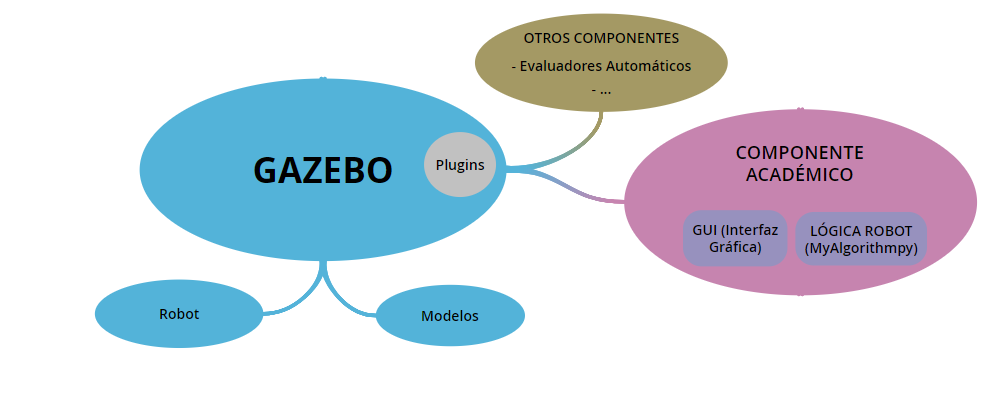
\includegraphics[width=0.9\linewidth]{figures/estructura_jde.png}
		\caption{Estructura de una práctica en JdeRobot-Academy}
		\label{fig.estructura}
		\end{center}
\end{figure}

Como se ha descrito anteriormente, en la Figura 1.4 se puede apreciar que la arquitectura software de las prácticas académicas facilita el desarrollo de las mismas por parte de los alumnos de manera que sólo se concentran en el desarrollo del algoritmo con la lógica del robot. El componente académico es el encargado de cargar en el simulador el código desarrollado por el alumno desde el fichero \textit{MyAlgorithm.py} y visualizar trazas que ayuden a la depuración del código como las imágenes procesadas, datos del láser o imágenes de la cámara integrada, dependiendo de la práctica.

El entorno usual para la realización de las prácticas es el simulador Gazebo, aunque las prácticas se han desarrollado de manera que puedan ser soportadas por robots reales sin realizar ninguna modificación, con los correspondientes drivers del robot. Gracias a esto, el código puede ser probado en robots reales. El sistema operativo base sobre el que se han desarrollado las prácticas es Linux dado que presenta una interfaz más sencilla a la hora de programar, por ello Linux cuenta con toda la infraestructura de las prácticas. 
Aunque en la actualidad se está terminando el entorno JdeRobot-Academy-Web en el que las prácticas docentes están almacenadas en un servidor y se puede acceder a ellas mediante el navegador. De esta manera se convierte al entorno JdeRobot en multiplataforma dotándolo de mayor accesibilidad. Esto es gracias al desarrollo de la interfaz web de Gazebo para la simulación, a la plataforma Jupyter (ver 3.6) que, mediante sus cuadernillos, han permitido trasladar las prácticas de JdeRobot-Academy al entorno docente JdeRobot-Academy-Web y al empleo de Dockers para dotar el entorno de un soporte multiplataforma.

Algunas de las prácticas que componen la plataforma son los siguientes:

\hspace{0.4\linewidth}
\textit{Follow Line}

\begin{figure}[H]
  \begin{center}
    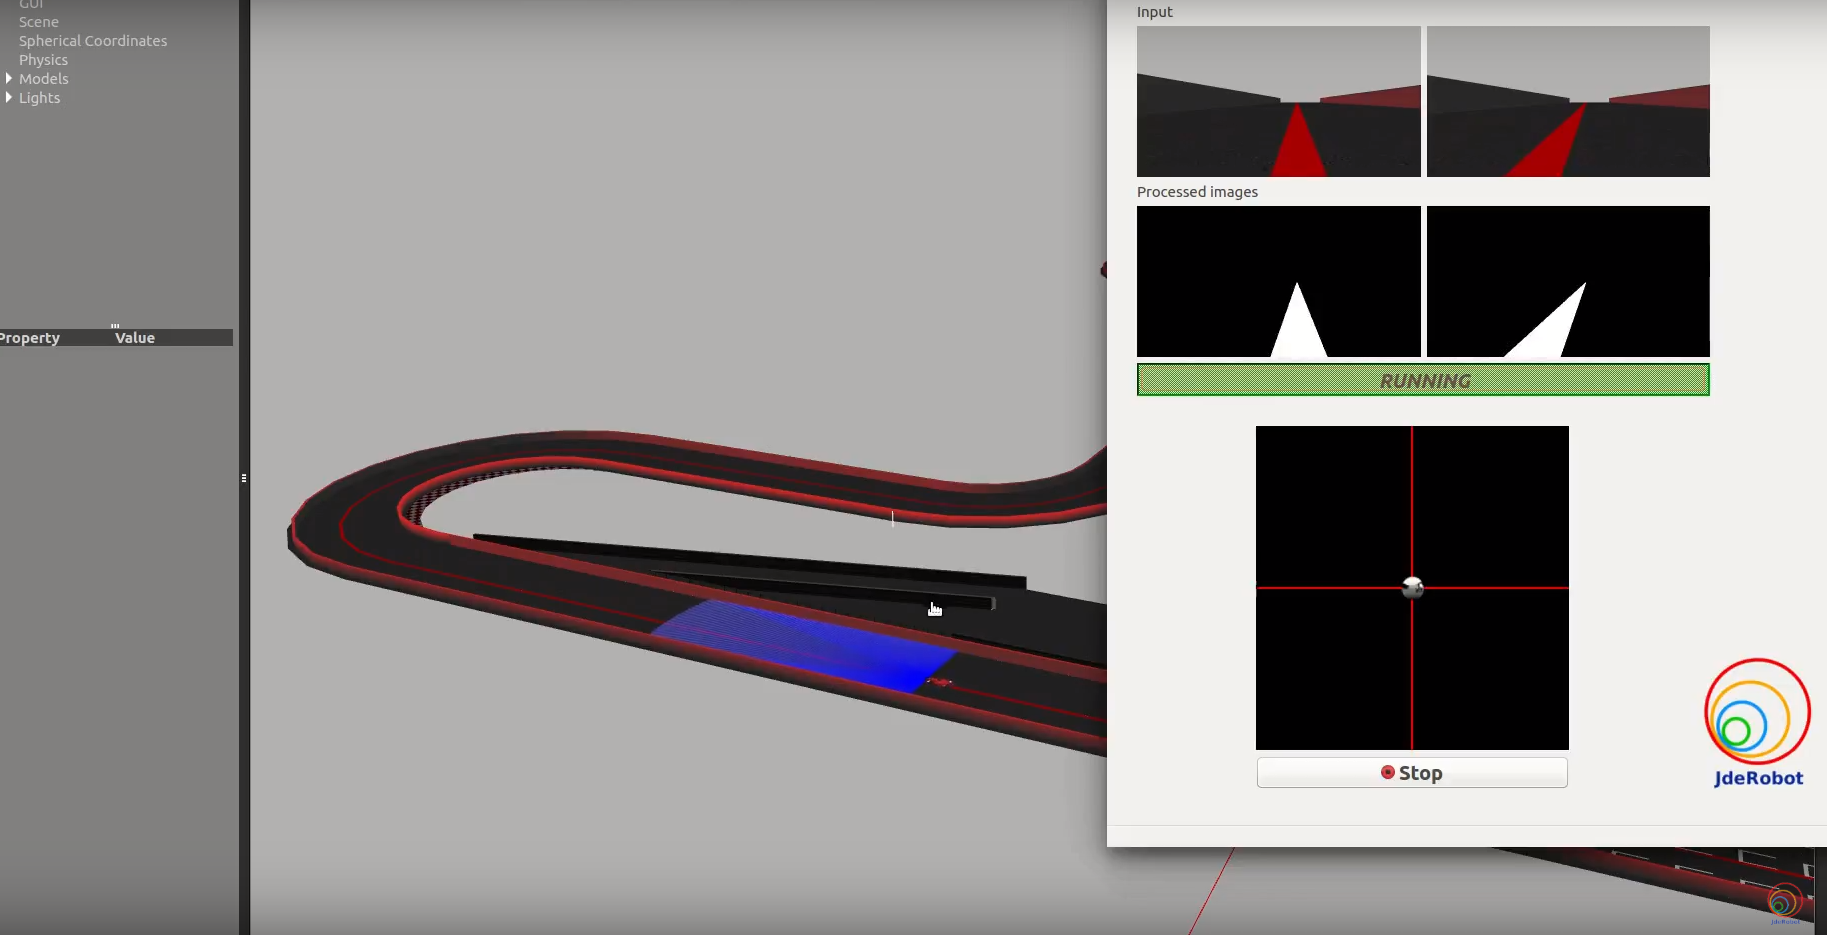
\includegraphics[width=0.95\textwidth]{figures/followline.png}
		\caption{Follow Line}
		\label{fig.followline}
		\end{center}
\end{figure}

Este ejercicio \textit{Follow Line} (Figura 1.5) trata de un robot coche Fórmula1 que consta de una cámara en su parte frontal por la que recoge imágenes. En su código se deben recoger las imágenes y procesarlas de manera que filtre la línea roja del circuito y la siga hasta que complete el circuito por completo \footnote{\url{https://youtu.be/QGO9oaoBVoA}}.

\vspace{4cm}
\hspace{0.40\linewidth}
\textit{Vacuum Cleaner}

\begin{figure}[H]
  \begin{center}
    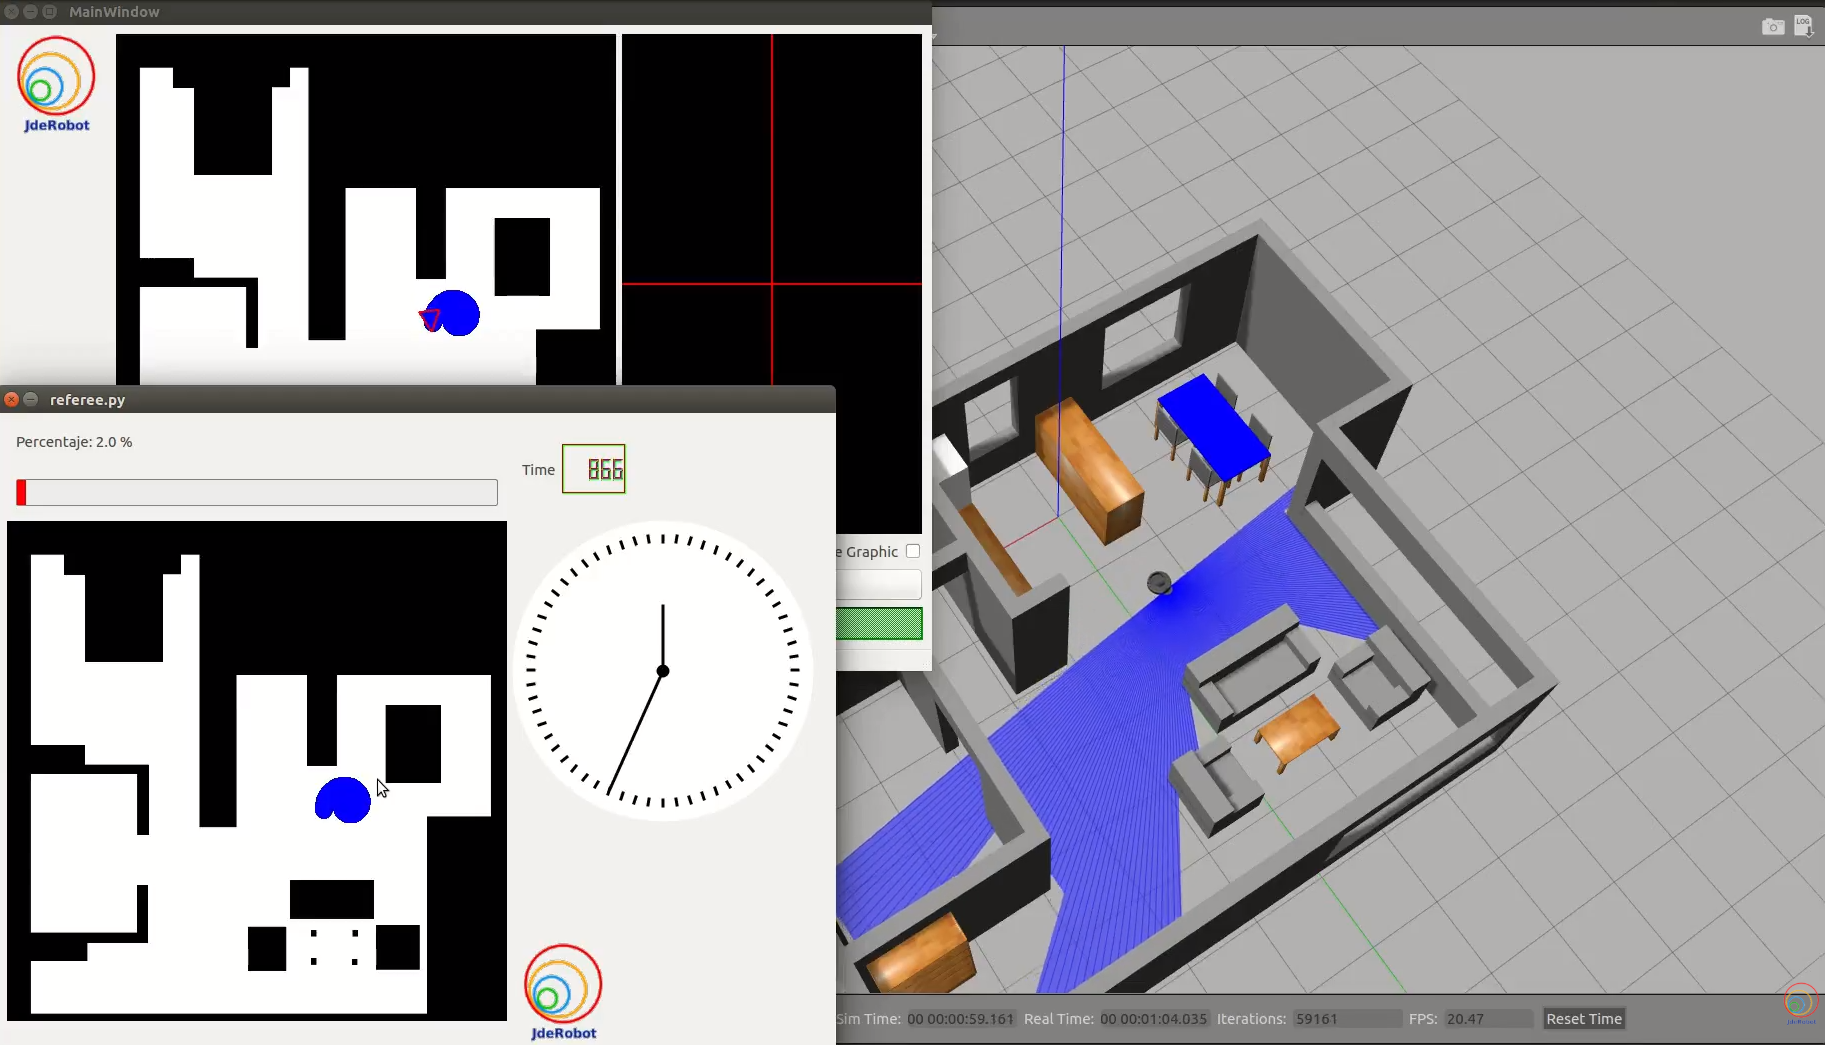
\includegraphics[width=0.50\linewidth, height=5cm]{figures/vacuumcleaner.png}
		\caption{Vacuum Cleaner}
		\label{fig.vacuumcleaner}
		\end{center}
\end{figure}

En este ejercicio \textit{Vacuum Cleaner} (Figura 1.6), el alumno debe recoger los datos del láser incluido en el modelo del robot aspiradora Roomba para que pase por el mayor área posible del escenario evitando la colisión con los obstáculos contenidos \footnote{\url{https://youtu.be/12muuY9JXLk}}.

\vspace{4cm}
\hspace{0.40\linewidth}
\textit{Visual Lander}

\begin{figure}[H]
  \begin{center}
    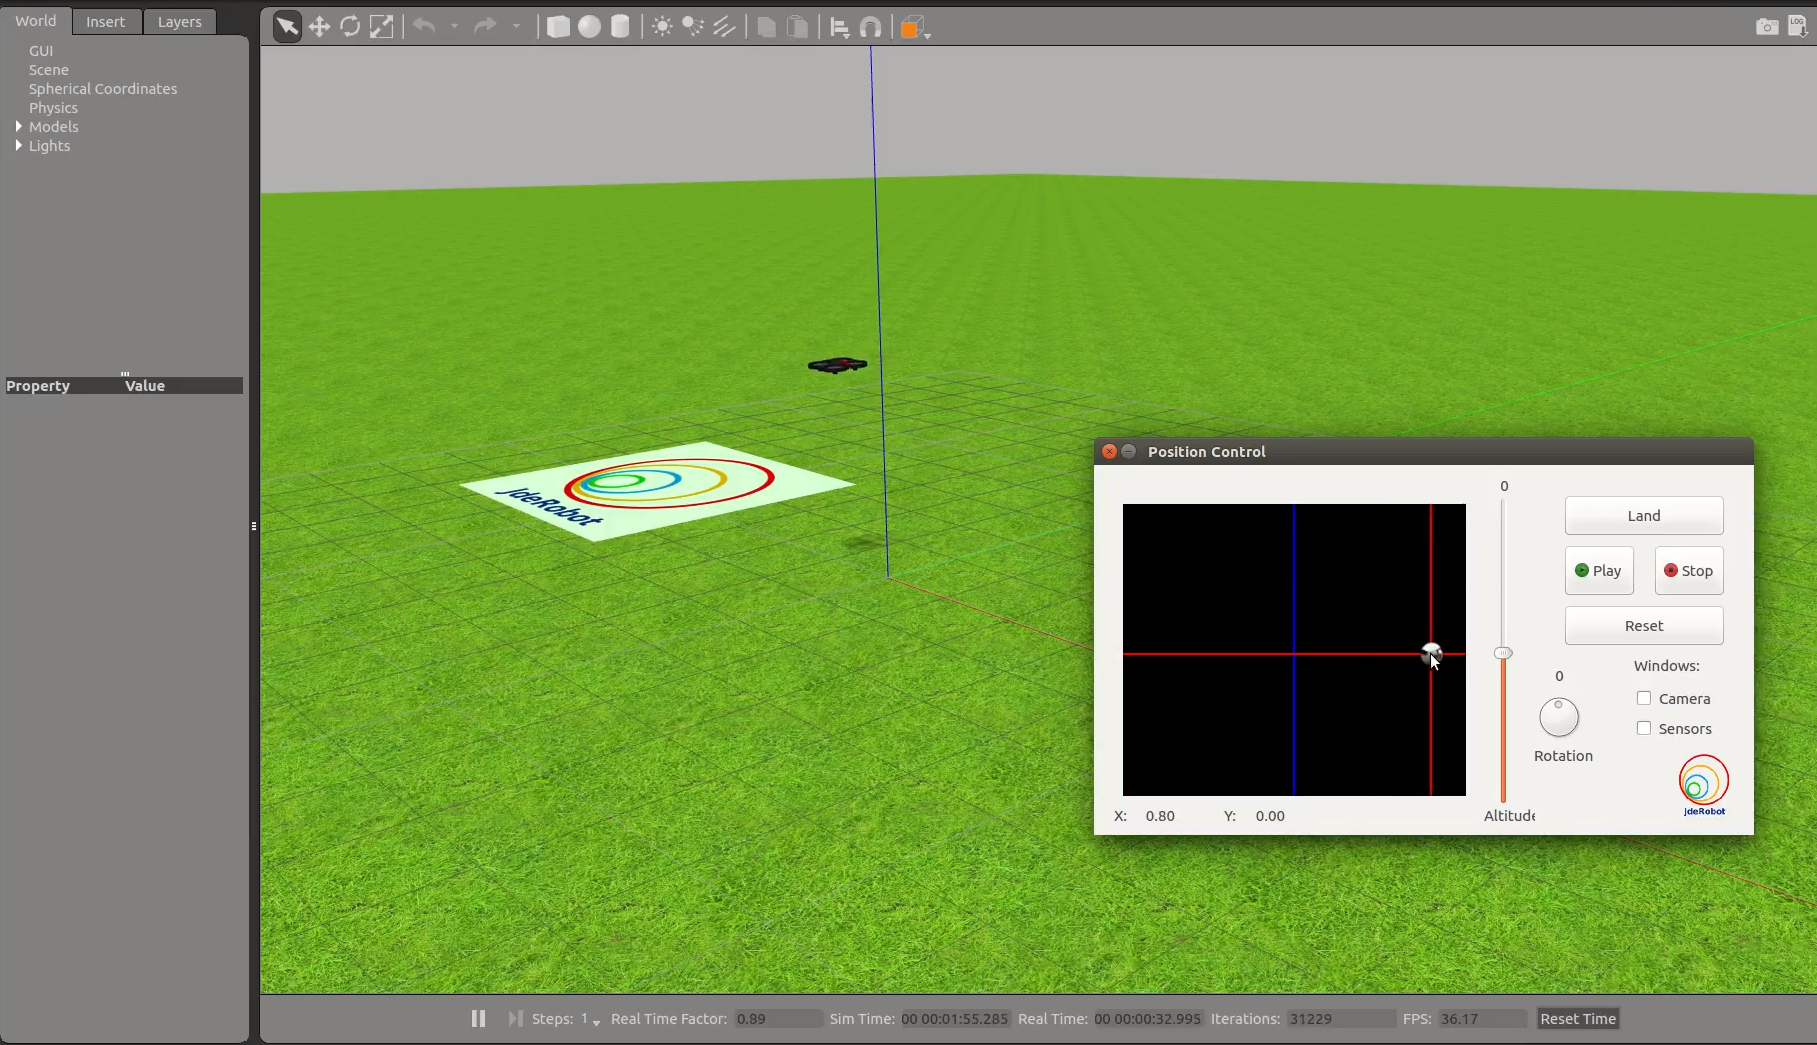
\includegraphics[width=0.50\linewidth, height=5cm]{figures/visuallander.png}
		\caption{Visual Lander}
		\label{fig.visual lander}
		\end{center}
\end{figure}

En este ejercicio \textit{Visual Lander} (Figura 1.7), el alumno deberá programar la lógica de un dron para que filtre las imágenes captadas por su cámara ventral y filtrarlas para distinguir una baliza y aterrizar controladamente sobre ella \footnote{\url{https://youtu.be/36pwaFYmDD0}}.

\vspace{4cm}
\hspace{0.40\linewidth}
\textit{Follow Turtlebot}

\begin{figure}[H]
  \begin{center}
    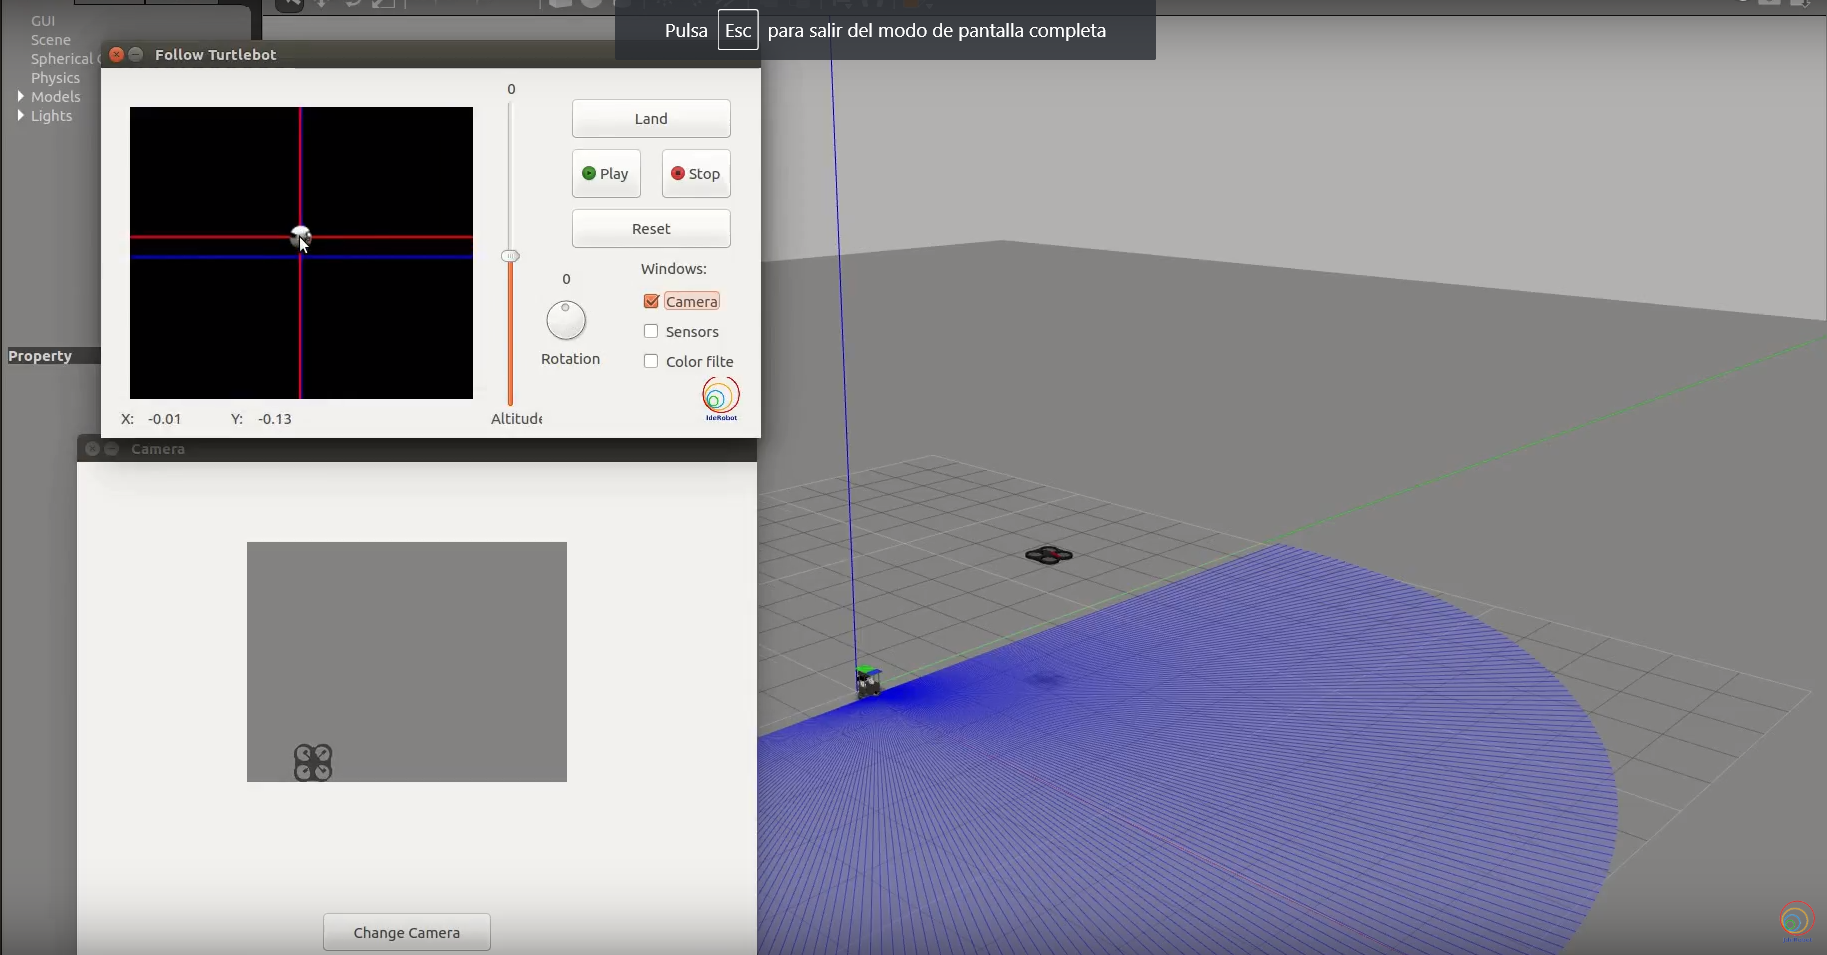
\includegraphics[width=0.50\linewidth, height=5cm]{figures/followturtlebot.png}
		\caption{Follow Turtlebot}
		\label{fig.followturtlebot}
		\end{center}
\end{figure}

Este ejercicio \textit{Follow Turtlebot} (Figura 1.8), consta de un escenario con un robot turtlebot teleoperado por el alumno y un dron. El código del algoritmo deberá dotar la inteligencia necesaria al dron para recoger las imágenes captadas por la cámara ventral del dron y filtrarlas para reconocer la baliza que lleva el turtlebot en su parte superior. Una vez reconocida debe dotar al dron de movimientos para seguirlo \footnote{\url{https://youtu.be/uehDVlBzpmU}}.

\vspace{7cm}
\hspace{0.35\linewidth}
\textit{Drone-Cat-Mouse}

\begin{figure}[H]
  \begin{center}
    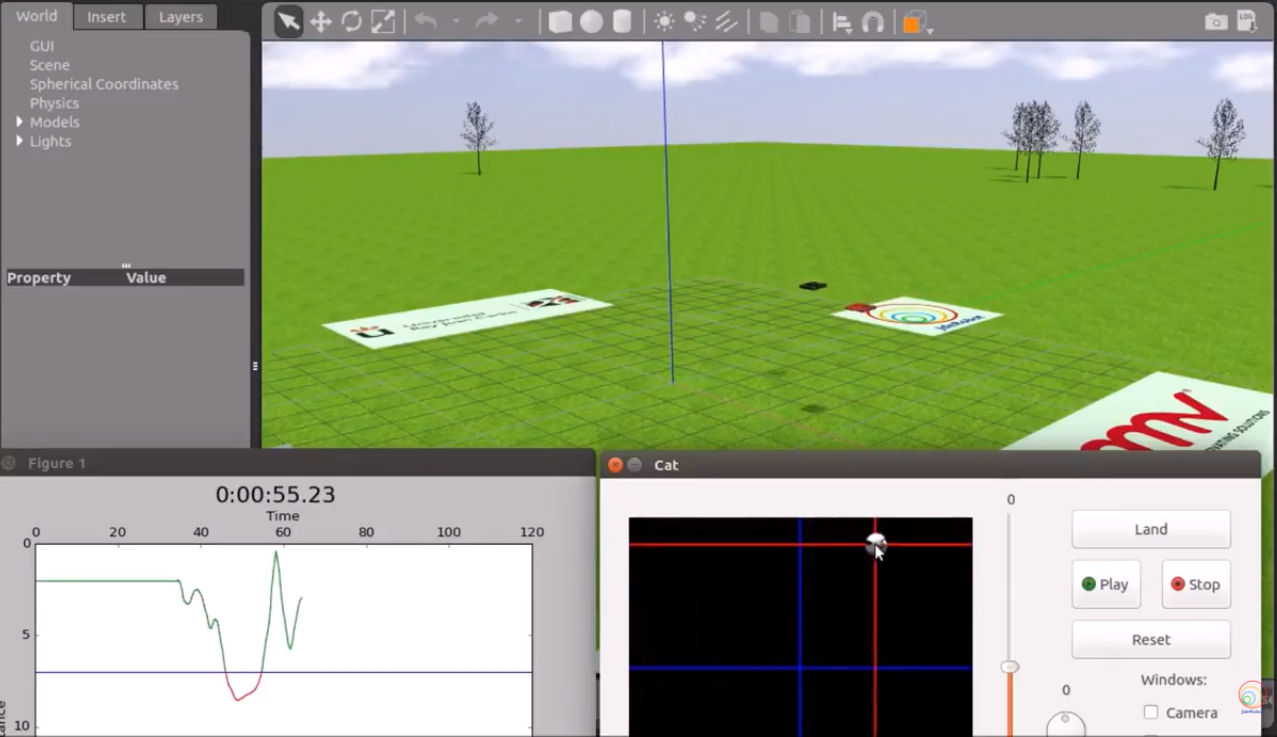
\includegraphics[width=0.95\textwidth, height=7.2cm]{figures/dronecatmouse.png}
		\caption{Drone-Cat-Mouse}
		\label{fig.dronecatmouse}
		\end{center}
\end{figure}

\textit{Drone-Cat-Mouse} es una de las prácticas más complejas del entorno JdeRobot-Academy. En ella el alumno debe dotar de la lógica necesaria a un dron (dron negro) para recoger las imágenes captadas por su cámara y filtrarlas para encontrar a un dron rojo. Una vez reconocido el dron rojo debe dotar de movimiento al dron para perseguirlo dado que el dron rojo está en movimiento. El objetivo es que el dron negro se acerque los más posible al dron rojo pero sin colisionar con él emulando el juego Gato-Ratón\footnote{\url{https://www.youtube.com/watch?v=DYD9oPawhWg}}. Esta práctica se ha utilizado en las dos ediciones del campeonato \textit{Program-A-Robot}, la primera en la URJC y la segunda en las Jornadas Nacionales de Robótica. Se va a utilzar en la tercera edición que tendrá lugar en la conferencia internacional IROS\footnote{\url{https://www.iros2018.org/competitions}}.

\subsection{Ejercicios recientes}

El contexto imediato de este Trabajo de Fin de Grado consiste en una serie de ejercicios elaborados recientemente  para enriquecer el contenido del entorno JdeRobot-Academy.

Entre los ejercicios elaborados más actuales caben destacar el TFG de Irene López Rodríguez \textit{"Nuevas Prácticas en el Entorno Docente de Robótica JdeRobot-Academy"}\cite{tfg1} en el que se introdujeron dos prácticas nuevas llamadas Coche autónomo negociando un cruce y Aspiradora autónoma con autolocalización. El primer ejercicio, después llamado \textit{Car Joint} trata sobre un coche autónomo que realiza un cruce por el que circulan coches. Para ello el coche debe filtrar las imágenes para reconocer una señal de Stop, así como los coches que circulan y las líneas de los carriles. Cuando no detecte ningún coche circulando debe tomar la intersección y escoger el carril correcto. La segunda práctica es similar a la práctica \textit{Vacuum Cleaner} pero consta del mapa con el escenario y sensor de posición, de manera que la aspiradora debe saber en qué lugar del escenario se encuentra y no repetir áreas ya limpiadas.

Otro TFG destacado en este aspecto es el de Vanessa Fernández Martínez \textit{{“Nuevas Prácticas en el Entorno Docente de Robótica JdeRobot-Academy”}}\cite{tfg2}, en el cual se añadieron dos prácticas nuevas llamadas Aspiradora Autónoma o \textit{Vacuum Cleaner} y Aparcamiento Automático, además de mejorar la práctica Tele Taxi con nuevos modelos, un mejor rendimiento del algoritmo GPP de navegación global y la inclusión de un evaluador automático capaz de medir el desempeño del algoritmo y proporcionar una nota. En cuanto al ejercicio desarrollado \textit{Vacuum Cleaner} ya ha sido comentado en el apartado anterior. La segunda práctica llamada \textit{Autopark} tiene como objetivo el aparcamiento de un coche autónomo mediante mediciones láser de los sensores frontales, laterales y posteriores.

También hay que mencionar el Trabajo de Fin de Grado desarrollado por Carlos Awadallah Estévez \textit{“Nuevas Prácticas Docentes de Robótica en el  Entorno JdeRobot-Academy”}\cite{tfg3}, en el cual se incorporan dos nuevas prácticas al entorno JdeRobot-Academy. La primera de ellas llamada \textit{Follow Face} trata de dar la lógica necesaria a una cámara pantilt de manera que procese las imágenes captadas por la cámara y reconozca la cara. Una vez hecho esto debe seguir el movimiento de la cara. La segunda práctica que se desarrolla en este TFG se llama \textit{Laser Loc} en la cual mediante mediciones de los sensores laser y un mapa con el escenario es capaz de realizar estimaciones de posición mediante movimiento y odometría.

Siguiendo con esta filosofía, el presente Trabajo de Fin de Grado aporta una práctica totalmente nueva al entorno JdeRobot-Academy y una optimización y mejora global de una práctica obsoleta incluyéndola en el entorno JdeRobot-Academy-Web.

\vspace{3cm}

El objetivo de este TFG es ampliar la variedad de prácticas que forman el entorno JdeRobot-Academy desarrollando nuevas prácticas y mejorando las exitentes para aumentar su versatilidad, además de aportar en el elenco de prácticas de JdeRobot-Academy-Web para acercar al entorno a dar soporte multiplataforma. En los próximos capítulos serán abordados los elementos necesarios para conseguir este objetivo. Comenzaremos con el Capítulo 2, en el que se concretarán los objetivos marcados, así como el punto de partida de este TFG y la metodología que ha sido empleada. En la Capítulo 3 se abordará la infraestructura utilizada para realizar el proyecto. En los Capítulos 4 y 5 explicaremos las prácticas que se han abordado en este TFG. Y, por último, en el Capítulo 6, se expondrán las conclusiones obtenidas, además de las posibles líneas de mejora futuras.


\lhead[]{CAP\'ITULO \thechapter. OBJETIVOS}
\chapter{Objetivos}\label{cap.objetivos}
Una vez introducido el contexto en que se ha desarrollado este trabajo, es hora de profundizar en los objetivos que se han tratado de alcanzar, los requisistos para las soluciones desarrolladas y la metodología que se ha seguido para conseguirlos.

\section{Objetivos}
La meta alcanzada en este preyecto es el desarrollo de una nueva práctica de sisemas robóticos para el entorno docente de JdeRobot-Academy llamada \textit{Chrono} y la optimización de una práctica existente llamada \textit{Follow Road}, así como una actualización de sus drivers para que soporte ROS y su inclusión en la infraestructura web de JdeRobot-Academy-Web.

La primera práctica consiste en la competición de dos coches de F1 por un circuito que dispone de una línea roja que se debe seguir. El código del alumno competirá con el F1 del mejor tiempo registrado para el circuito en el que esté compitiendo. De esta manera consguiremos que el alumno pueda depurar su código de solución y tenga un estímulo para alncanzar la perfección en el desarrollo de su algoritmo.

En cuanto a la segunda práctica, trata de un dron con con una cámara que debe seguir una carretera. El código del alumno deberá filtrar las imágenes para segmentar la carretera y dotar de un movimiento conttrolado al dron que le permita seguir la carretera.

\section{Requisitos}
A continuación se van a enumerar los requisitos necesarios para proporcionar soporte al software desarrollado:

\begin{enumerate}
	\item El Sistema Operativo empleado será Ubuntu 16.04 LTS.
	\item Se utilizará el \textit{middleware} robótico JdeRobot en su versión 5.6.2. El uso de este \textit{middleware} robótico simplifica el desarrollo del comportamiento del robot.
	\item Se usará \textit{OpenCV3} para la filtración de las imágenes captadas por las cámaras en ambas prácticas.
	\item Para dar soporte a los sensores y actuadores se utilizará \textit{ROS-Kinetic}.
	\item Para mostrar el comportamiento de los robots y el desarrollo de un mundo que los soporte se utilizará el simulador \textit{Gazebo}.
	\item El lenguaje de programación utilizado para el desarollo de ambas prácticas será \textit{Python} en su versión 2.7.12, por compatibilidad con el \textit{middleware} robótico JdeRobot y con el \textit{middleware ROS-Kinetic}.
	\item Las soluciones desarrolladas deben ejecutar algoritmos en tiempo real, por lo que deben ser eficientes y realizar movimientos suaves.
\end{enumerate}

\section{Metodología}
El desarrollo de este Trabajo de Fin de Grado puede descomponerse en un conjunto de iteraciones con distintas fase. Cada fase está formada por una reunión semanal con el tutor para determinar los objetivos a abordar, la planificación de cómo abordarlos, intentar solucionar los problemas que vayan a surgir anticipadamente y la consecución de los objetivos durante la semana. De esta manera se ha coneguido un desarrollo fluido y completo, asentando los conocimientos y despejando las dudas que surgían durante los meses dedicados a este deesarrollo.

Además de las reuniones semanales, se han utilizado herramientas de apoyo como la bitácora semanal en la Wiki de JdeRobot\footnote{\url{https://jderobot.org/Pablomoreno-tfg}}, donde se redactaban los avances obtenidos acompañados de vídeos demostrativos e imágenes. El código desarrollado se almacenaba, progresivamente, en la plataforma Github, en un repositorio personal\footnote{\url{https://github.com/RoboticsURJC-students/2017-tfg-pablo-moreno}} \footnote{\url{https://github.com/PabloMorenoVera/JdeRobot}} \footnote{\url{https://github.com/PabloMorenoVera/Academy}}, a los cuales el tutor tiene acceso para dar realimentación y orientar el proceso.

 El modelo de desarrollo escogido ha sido el modelo creado por Barry Boehm, dado que al tratarse de un modelo en espiral, se adaptada a la perfección a nuestras necesidades, permitiendo disponer de flexibilidad ante cambios en los requisitos semanales, algo común mientras avanzaba el desarrollo, a la par que nos permitía separar el objetivo final en varias sub-tareas más sencillas. Con esto se ha conseguido una subsanación de los riesgos temprana y la definición de una arquitectura en las fases iniciales del desarrollo, todo ello dotado con un control de calidad continuo.

\begin{figure}[H]
  \begin{center}
    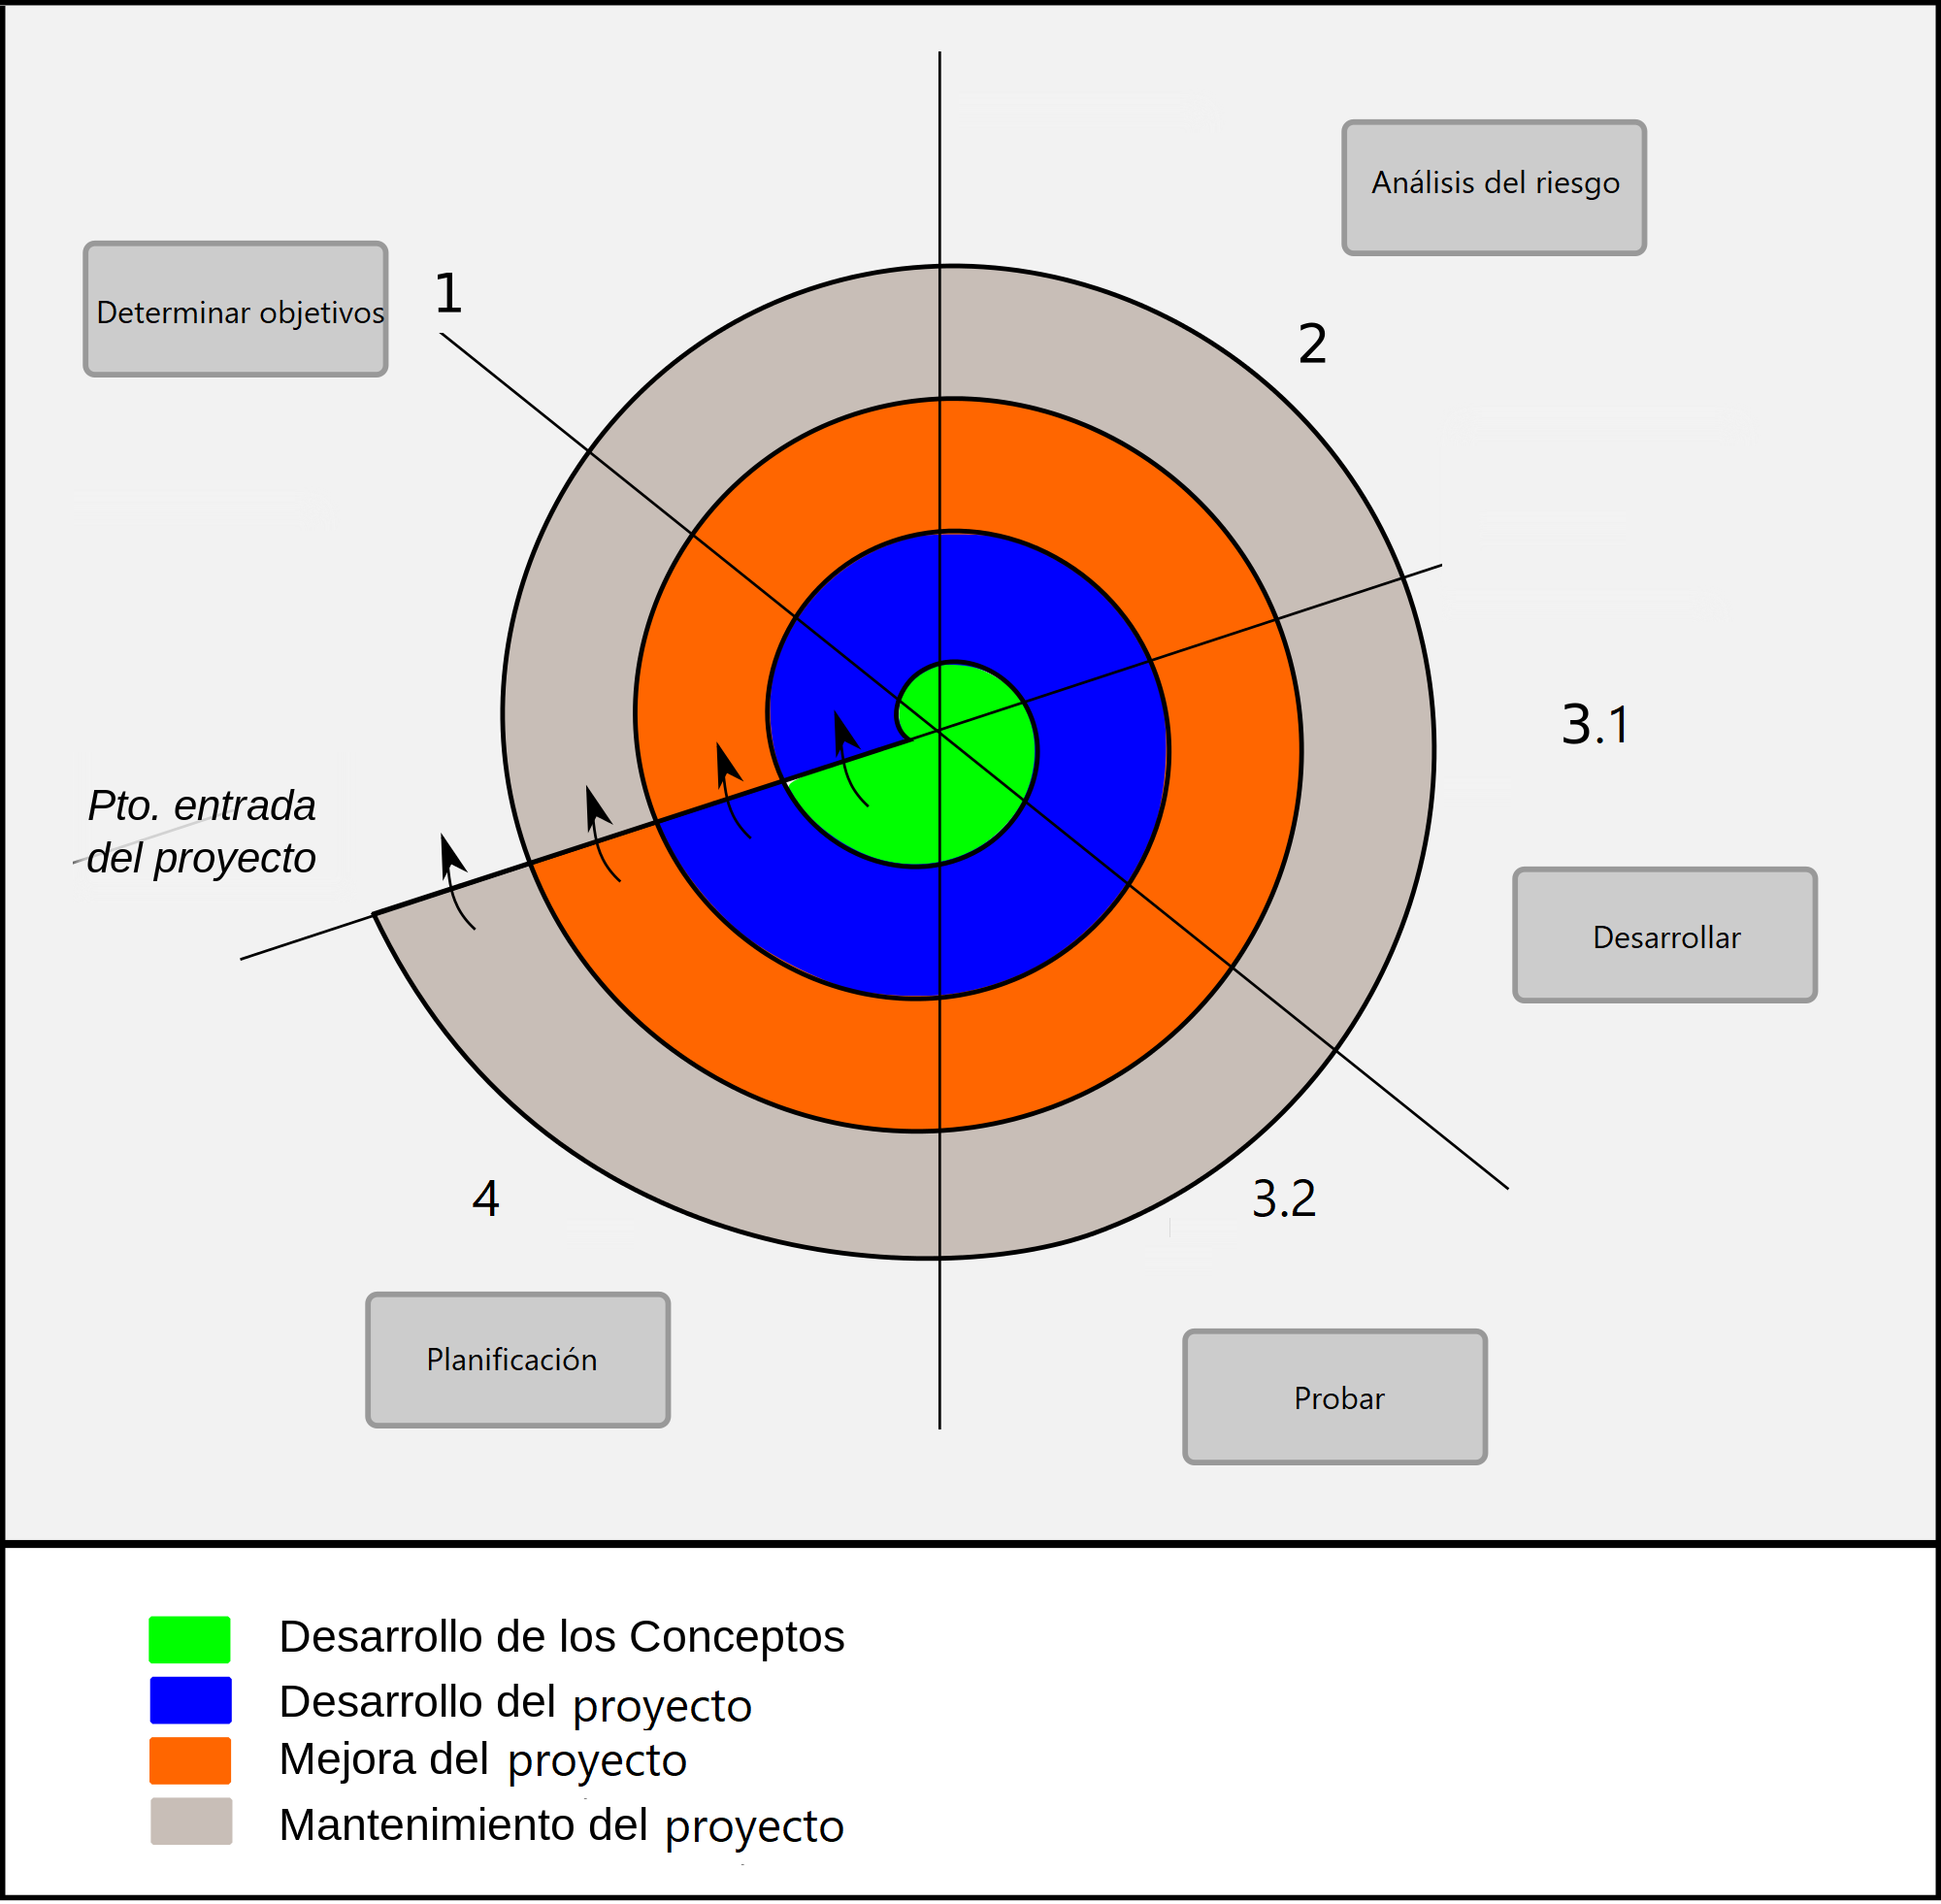
\includegraphics[width=0.9\linewidth]{figures/modelo_espiral.png}
		\caption{Modelo de desarrollo en espiral}
		\label{fig.espiral}
		\end{center}
\end{figure}

La ventaja de este ciclo de vida es que permite la obtenicón de prototipos funcionales en una etapa temprana, la optimización progresiva del prototipo desarrollado y, en última instancia, pulir los detalles para abarcar la totalidad de los requisitos especificados (Figura 2.1). De esta manera el trabajo se desarrolla de manera incremental con cuatro fases bien definidas:

\begin{itemize}
	\item[--] \textbf{Determinar objetivos}: Esta primera fase del ciclo está formada por la definición de las metas.
	\item[--] \textbf{Análisis del riesgo}: Se evalúan los posibles problemas iniciales al desarrollo y las soluciones a los mismos.
	\item[--] \textbf{Desarrollar y probar}: En esta tercera fase se procede al desarrollo del trabajo propiamente dicho, junto con una serie de pruebas para verificar su funcionamiento.
	\item[--] \textbf{Planificación}: En esta última fase del ciclo se valoran los resultados obtenidos y se planifican las siguientes etapas del proyecto.
\end{itemize}

\section{Plan de trabajo}
Para la consecución de los objetivos descritos, se han seguido las siguientes etapas de trabajo:

\begin{itemize}
	\item[--] \textbf{Familiarización con el entorno JdeRobot}: una vez descargado e instalado tanto el software, dependencias y bibliotecas como el simulador, se tomará un primer contacto con el entorno JdeRobot mediante la modificación y readaptación de algunas prácticas existentes, como sus interfaces gráficas.
	\item[--] \textbf{Toma de contacto con el simulador Gazebo}: esa etapa se ha dedicado al desarrollo de algunos modelos en el simmulador, estudiando ejemplos disponibles en la web\footnote{\url{http://gazebosim.org/tutorials}} y en JdeRobot, así como modificándolos y desarrollando algunos modelos nuevos (Figuras ~\ref{fig:estanteria} y ~\ref{fig:warehouserobot}). En esta etapa también se han estudiado el funcionamiento básico de los \textit{plugins} que dispone Gazebo para el control de sus robots, sensores y acutadores. Esto ha suspuesto una toma de contacto con el lenguaje de programación C++ utilizado, también, para comprender los \textit{plugins} de ROS-Kinetic.
\begin{figure}[H]
	\centering
	\begin{minipage}[h]{.48\linewidth}
		\centering
		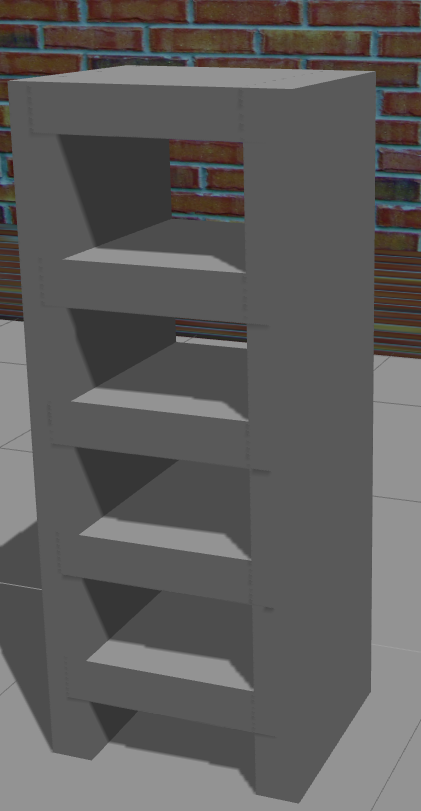
\includegraphics[width=.5\linewidth, height=7cm]{figures/estanteria.png}
		\captionof{figure}{Modelo estantería}
		\label{fig:estanteria}
	\end{minipage}
	\begin{minipage}[H]{.48\linewidth}
		\centering
		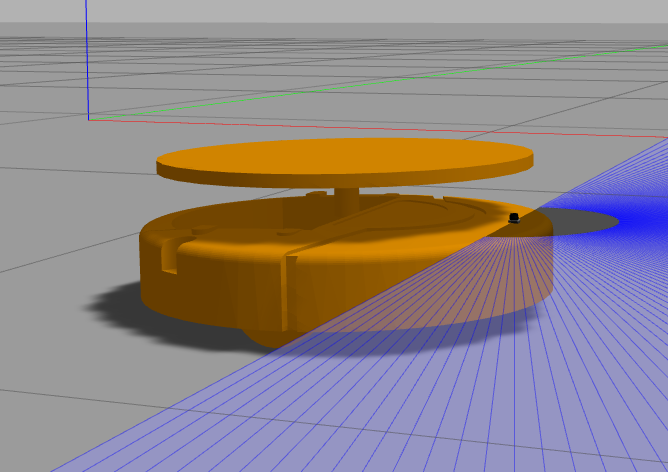
\includegraphics[width=.7\linewidth, height=7cm]{figures/warehouse_robot.png}
		\captionof{figure}{Warehouse robot}
		\label{fig:warehouserobot}
	\end{minipage}
\end{figure}
	\item[--] \textbf{Estudio de las bibliotecas}: En este punto fue necesario el estudio de diferentes bibliotecas disponibles en python para poder comenzar con el desarrollo de las prácticas. Fue necesario el estudio de bibliotecas como \textit{OpenCV}, Threading, Numpy y PyQt5.
	\item[--] \textbf{Optimización de la práctica del sigue carretera}: Esta práctica estaba bastante obsoleta y se procedió a renovar por completo su interfaz gráfica, el escenario utilizado incluyendo un nuevo dron que soportaba ROS y una nueva conexión de los sensores y actuadores del propio dron. Además se desarrolló una optimización global del nodo académico como la inclusión de una pausa académica. Además se creó una versión de la práctica para la plataforma Jupyter y se incluyó en el elenco de práticas soportadas en JdeRobot-Academy-Web.
	\item[--] \textbf{Desarrollo de una solución de referencia para la práctica}.
	\item[--] \textbf{Preparación de la infraestuctura del ejercicio chrono}: Se desarrollará el modelo del F1 y el circuito para competir en \textit{Blender} y \textit{SketchUp} para conformar el escenario de Gazebo. También se desarrollarán los drivers del robot F1 para dar soporte en ROS-Kinetic de los motores. la cámara y el láser. Se creará el noodo académico de la práctica para alojar el código del estudiante y la versión de la práctica para Jupyter.
	\item[--] \textbf{Desarrollo de una solución de referencia para chrono}.
\end{itemize}
\lhead[]{CAP\'ITULO \thechapter. INFRAESTRUCTURA}
\chapter{Infraestructura}\label{cap.infraestructura}
En este capítulo tratará de abordar todos los componentes y software que han servido de apoyo en el desarrollo del TFG. En este punto daremos una explicación detallada sobre las plataformas en las que se cimienta el trabajo (ROS y JdeRobot), en el simulador Gazebo, en los editores de modelos, en las librerías más importantes (OpenCV y PyQt), en el proyecto Jupyter y en el entorno JdeRobot-Academy-Web.

\section{Entorno ROS}
ROS (Robot Operating System) proporciona a los desarrolladores de software robótico los componentes necesarios para el desarrollo de aplicaciones robóticas. Entre ellos destacan la abstracción hardware, bibliotecas, intercambios de mensajes, administración de paquetes, controladores de dispositivo y visualizadores. Esta plataforma se distribuye en código abierto bajo una licencia BSD.

Una de las características más importantes de ROS es su integración con el simulador Gazebo, con el que se comunica a través de paquetes llamados \textit{gazebo\_ros\_pkgs} \footnote{\url{http://ros.org/wiki/gazebo\_ros\_pkgs}}. Mediante estos paquetes, ROS es capaz de proporcionar las interfaces necesarias para simular un robot en Gazebo usando \textit{ROS Messages}, servicios y reconfiguración mecánica.

Esta plataforma se conforma como una colección de nodos o procesos que suponen una computación. Los nodos se combinan en un gráfico y se comunican entre sí mediante \textit{topics} de transmisión, servicios RPC y el Servidor de Parámetros. Un sistema de control de un robot se formará por la integración de distintos nodos, cuanto mayor sea la funcionalidad de la que se dote al robo, mayor número de nodos tendrá. Existen nodos de control de láser, vista gráfica del sistema, motores de ruedas, odometría, cámaras, etc. La existencia de nodos de ROS en el robot proporciona beneficios para el sistema robótico como tolerancia adicional a fallos soportados por cada nodo de manera indivual, de esta manera el fallo se concentra en un solo nodo. Además, la complejidad del código se reduce con los sistemas monolíticos.

Los \textit{topics} de ROS actúan como forma de comunicación, de esta manera se definen como buses sobre los que los nodos intercambian mensajes. Gracias a la semántica de publicación y/o suscripción anónima de los \textit{topics}, se desacopla la producción de información de consumo. Debido a esto los nodos no saben con quién se están comunicando. Por otra parte, los nodos interesados en un \textit{topic}, se suscriben a él para recoger la información que se publique por el mismo y, por otra parte, los nodos que generen datos pertenecientes a ese \textit{topic}, transmitirán la información por él. Es importante destacar que puede haber varios editores o generadores y varios suscriptores del mismo \textit{topic}.

Debido a la compatibilidad de ROS con Gazebo y con JdeRobot, se pueden utilizar los \textit{plugins} de ROS para las simulaciones en Gazebo de las prácticas presentes en el entorno JdeRobot mediante el establecimiento de las conexiones de los sensores y actuadores de la práctica con los \textit{plugins} de ROS en el nodo académico de la misma.

Existen una gran cantidad de \textit{plugins} de ROS que proporcionan una enorme diversidad de funcionalidad para el desarrollo de robots \footnote{\url{http://wiki.ros.org/gazebo_plugins}}. Entre ellos destacan el plugin que controla el láser, llamado \textit{libgazebo\_ros\_laser} o el que controla una cámara, llamado \textit{libgazebo\_ros\_camera}. Ambos plugins serán usados en las prácticas contenidas en este Trabajo de Fin de Grado.

\section{JdeRobot}
La plataforma \textit{JdeRobot}\footnote{\url{http://jderobot.org}} es un \textit{middleware} abierto para desarrolladores de robots y visión artificial. Fue creada por el Grupo de Robótica de la Universidad Rey Juan Carlos en 2003 y está licenciada como GPLv3\footnote{\url{https://www.gnu.org/licenses/quick-guide-gplv3.html}}.
La estructura de esta plataforma ha sido desarrollada en C y C++, aunque tiene componentes escritos en Python y JavaScript. El entorno ofrecido es mediante componentes, los cuales son ejecutados como procesos que interoperan entre sí mediante \textit{middleware} de comunicaciones como ICE o \textit{ROS-Messages}, que permiten la interoperación de componente en un entorno multilenguaje.

JdeRobot facilita los \textit{drivers} necesarios para la funcionalidad de sus robots. De esta manera, los \textit{dirvers} están asociados al hardware del robot proporcionando interfaces de acceso, por lo que simplifica la comunicación de las aplicaciones con los actuadores del robot que se realiza mediante una función mediante los interfaces ICE o ROS.

Los dispositivos que se pueden encontrar en JdeRobot son muy diversos, destacan el cuadricópteros como el Ardronde de Parrot, operativo con ICE, o el SoloDrone de 3DR, operativo con ROS, los coches Fórmula1 desarrollados por la propia plataforma JdeRobot que incluyen modelos de la mayoría de las escuderías presentes en la Fórmula 1, operativos con ROS y modificados en este TFG para incluirlos en la plataforma. También se incluyen modelos como el boto Kobuki de Yujin Robot, el humanoide NAO de Aldebaran Robotics, cámaras fireware, USB e IP, los simuladores Stage y Gazebo, escáneres láser LMS de SICK y URG de Hokuyo, sensores de profundidad como Kinect y otros dispositivos X10 de domótica o \textit{drivers} específicos de control de cámaras, láser y motores de movimiento.

JdeRobot incorpora librerías de software libre para su uso como OpenCV para visión, Eligen para álgebra o PCL para manejo de nubes de puntos. Al ser compatible con ROS, en específico con ROS-Kinetic, las aplicaciones de la plataforma pueden incorporar nodos de ROS y conectarse a ellos de manera fluida.

Las prácticas que componen este Trabajo de Fin de Grado se han desarrollado en la versión de JdeRobot 5.6.2, última versión estable.

\section{Simulador Gazebo}
Gazebo\footnote{\url{http://gazebosim.org/}} es un simulador de robótica que permite emular escenarios tridimensionales para robots autónomos (Figura 3.1). Es apropiado para comprobar algoritmos basados en visión artificial y elusión de objetos. Al desarrollar algoritmos de control de robots es necesaria la realización de pruebas del software para confirmar la validez del código escrito. Es por ello que Gazebo adquiere una gran importancia como simulador, dado que permite probar la eficacia del código sin necesidad de probarlo con hardware real, pudiendo dañarlo. De esta manera los simuladores son importantes en la robótica, dado que permiten abaratar costes evitando los daños en el hardware del robot.

El simulador utilizado en el presente Trabajo de Fin de Grado es Gazebo, al ser de código abierto, versátil (capaz de simular objetos, robots y sensores en entornos complejos de interior y exterior), al posees una interfaz de gran calidad y un robusto motor de físicas (pueden describirse componentes como la masa, rozamientos, inercia, amortiguamiento, etc.). Fue elegido para soportar el DARPA Robotics Challenge de 2012 a 2015 y está mantenido por la Fundación Open Robotics\footnote{\url{https://www.openrobotics.org/}}

\begin{figure}[H]
  \begin{center}
    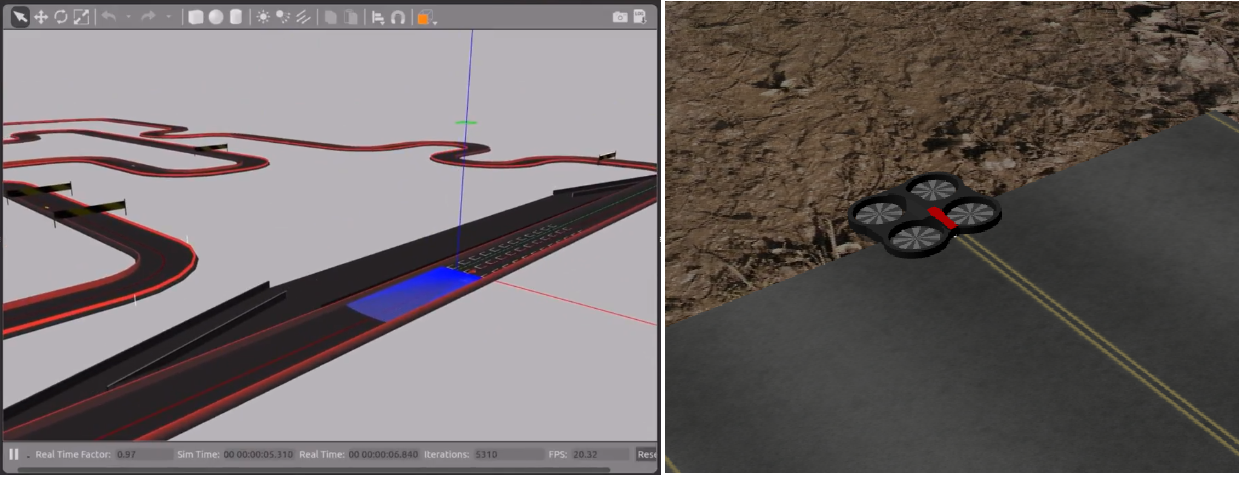
\includegraphics[width=0.9\linewidth]{figures/gazeboworlds.png}
		\caption{Ejemplo de mundo y modelo de Gazebo}
		\label{fig.worlds}
		\end{center}
\end{figure}

Los escenarios de Gazebo se describen en fichero con extensión ".world", que son ficheros escritos en XML (Extensible Remarkable Language) de descripción de documentos, definidos en el lenguaje de simulación SDF (Simulation Description Format), donde se recogen todos los elementos del escenario:

\begin{itemize}
	\item Escena: Iluminación, propiedades del cielo, sombras, etc.
	\item Mundo: Representación del mundo como conjunto de modelos, \textit{plugins} y propiedades físicas.
	\item Modelo: Componentes que forman el robot, como articulaciones, objetos de colisión, sensores, etc.
	\item Físicas: Gravedad, inercia, rozamiento, colisiones, motor físico, tiempo, etc.
	\item \textit{Plugins}: Pueden incluirse en el mundo, el modelo o un sensor. Pueden incluirse \textit{plugins} disponibles en la red como el que da soporte completo a la funcionalidad del robot Roomba, llamado \textit{libroombaplugin.so}.
\end{itemize}

Cada elemento del escenario cuenta con una etiqueta propia que lo distingue del resto. Cualquier propiedad descrita dentro de su etiqueta tiene que ir marcada con la etiquete de la propiedad correspondiente.
En la versión 7 de Gazebo se ha incluido un editor de modelos básico para poder desarrollar modelos y escenarios básicos. A partir de los modelos que se importen o desarrollen en Gazebo, es necesario adjuntar un \textit{plugin} que los dote de la funcionalidad necesaria, de otra manera no serían más que simples objetos inanimados.

\section{Editor de modelos}
Para el desarrollo del modelo de robots se ha trabajo con dos editores de modelos, SketchUp\footnote{\url{https://www.sketchup.com/}} y Blender\footnote{\url{https://www.blender.org/}}. Estos editores son necesarios para importar los modelos de robots generados en ellos al simulador Gazebo.
Existe un almacén web desde donde es posible descargarse una gran variedad de modelos y escenarios, además de desarrollar los propios. Una vez desarrollado el modelo o escenario, estos editores exportan el modelo o escenario en formato ".dae" (Digital Assets Exchange), formato perteneciente al lenguaje XML, y los correspondientes texturas en imágenes con formato ".JPG". Una vez obtenidos estos ficheros, ya son importables por el simulador Gazebo, pero es necesario una modificación para dotar al modelo o escenario de colisiones, inercias, gravedad, etc. 

Los escenarios y modelos generados por estos editores son creados mediante la intersección de líneas, generando los distintos tipos de objetos. Además, es posible adjuntar una textura o color a cada cara que forma el objeto. Además, el editor Blender, al ser más complejo, permite la introducción de iluminación y trabajar con formas geométricas en tres dimensiones directamente, en cambio el editor SketchUp trabaja con líneas, aunque es más sencillo de utilizar.

El editor de modelos Blender es de código abierto pero el editor de modelos SketchUp es de pago, pero tiene la ventaja de contar con su almacén de modelos en el que puedes descargar una gran variedad de modelos.

\section{Lenguaje Python}
Python\footnote{\url{https://www.python.org/}} es un lenguaje de programación orientado a objetos, interpretado y de alto nivel con semántica dinámica. Es un lenguaje de fácil aprendizaje y comprensión debido a su apariencia intuitiva. Su creador fue Guido van Rossum, un investigador holandés que trabajaba en el centro de investigación CWI (Centrum Wiskunde \& Informática. La primera versión de este lenguaje de programación surgió en 1991, pero no fue publicado hasta tres años después. El nombre que recibió este lenguaje fue dado por su creador en honor a la serie de televisión \textit{Monty Python's Flying Circus}.

La combinación del tipado y el enlace dinámico con sus estructuras de datos integradas de alto nivel, dotan a este lenguaje de un desarrollo rápido de aplicaciones, scripting o lenguaje de interconexión de componentes existentes. La sintaxis fácil y simple enfatiza su legibilidad y reduce el coste de mantenimiento del código. Además, Python admite módulos y paquetes, por lo que fomenta la modularidad del programa y la reutilización de código.

El intérprete de Python y la extensa biblioteca de paquetes están disponibles en formato binario o en código fuente de manera gratuita para las plataformas principales y pueden ser distribuidas libremente.

La última versión de Python Software Fundation es la 3.6.5. En este Trabajo de Fin de Grado hemos utilizado la versión 2.7.12, compatible con JdeRobot 5.6.2 y con ROS-Kinetic. De manera que la completitud de las dos prácticas desarrolladas en este trabajo está escrita en esta versión.

\section{Biblioteca OpenCV}
OpenCV\footnote{\url{https://opencv.org/}} (Open Source Computer Vision Library) es una librería de código abierto destinada al procesamiento de imágenes y el aprendizaje máquina. Fue desarrollada por Intel y publicada bajo licencia de BSD. El propósito de esta librería es facilitar el desarrollo de programas de visión por computador en tiempo real.

Se trata de una librería multiplataforma con soporte para MacOS, Linux, Android y Windows. Además, existen versiones en Java, Python y C\# a pesar de que era, originalmente, una librería en C/C++. También existen interfaces en desarrollo para Ruby, Matlab y otros lenguajes.
La librería OpenCV implementa algoritmos para técnicas de detección de rasgos, clasificación de acciones humanas en vídeos, reconocimiento, segmentación de objetos, calibración, seguimiento de caras, análisis de la forma y movimiento, reconstrucción 3D... Los algoritmo que componen esta librería están basados en estructuras de datos flexibles acoplados a estructuras IPL (\textit{Intel Image Processing Library}), utilizando la arquitectura de Intel respecto a la optimzación de la mayoría del paquete. También aprovecha la aceleración de cómputo gracias al uso de tarjetas gráficas avanzadas (GPUs). OpenCV fue desarrollado para tener una alta eficiencia computacional. Está escrito en el lenguaje de programación C y puede aprovechar las ventajas de los procesadores \textit{multicore} de nueva generación. Tales son las ventajas que aporta que las grandes compañías como Google, Yahoo, Microsoft, Intel, IBM, Sony, Toyota u Honda utilizan esta librería, que se ha convertido en el estándar de facto en su campo.

Para este trabajo se ha utilizado la librería OpenCV en la versión 3.2 y su ha sido empleada en toda la parte del código relacionada con tratamiento de imágenes.

\section{Biblioteca PyQt}
PyQt\footnote{\url{https://pypi.org/project/PyQt5/}} es un conjunto de enlaces Python utilizado para el conjunto de herramientas Qt, un \textit{framework} multiplataforma orientado a objetos y escrito en C++ que permite el desarrollo de interfaces gráficas. Incluye sockets, hilos, bases de datos SQL, Unicode, etc. Combina todas las ventajas de Qt y Python empleando todas las funcionalidades de Qt con un lenguaje de programación sencillo como es Python. Fue desarrollada por Riverbank Computing Ltd y tiene suporte multiplataforma con versiones para Windows, Linux, Mac OS X, iOS y Android.

Para este proyecto se ha utilizado la versión 5 de PyQt. Se trata de un conjunto de enlaces Python para Qt5, con soporte para Python 2.x y Python 3.x. Incluye más de 6000 funciones y 620 clases y métodos. Dispone de una licencia dual, es decir, puede elegirse una licencia comercial para usuarios o una licencia GPL (General Public Licence) para desarrolladores.
Las clases de PyQt5 se dividen en módulos: QtCore, QtGui, QtWidgets, QtXml y QtSql, entre otros. Para las prácticas desarrolladas, se han utilizado los siguientes módulos:
\begin{itemize}
	\item QtGui: contiene clases para la creación de interfaces gráficas y el desarrollo de gráficos en 2D, imágenes, texto y desarrollo de ventanas.
	\item QtCore: incorpora las clases principales no relacionadas con la interfaz gráfica. Se utiliza para trabajar con archivos, hilos, datos, procesos, urls, etc.
	\item QtWidgets: está formado por clases que proporcionan distintas funcionalidades a la interfaz del usuario.
\end{itemize}

\section{Jupyter}
Jupyter Notebook\footnote{\url{http://jupyter.org/}} se trata de una aplicación web de código abierto que permite al usuario desarrollar y compartir documentos que contengan código empotrado, ecuaciones, textos y visualizaciones. Proporciona una gran variedad de ventajas entre las que destacan limpieza, simulación numérica, modelado estadístico, visualización y transformación de datos, aprendizaje automático, etc. Inicialmente fue desarrollado como IPython 3.0 pero se renombró como Jupyter.

El cuadernillo de trabajo o \textit{Notebook} está compuesto por celdas en las que se inserta el código, en lenguaje Python, o distintos elementos de texto enriquecido como párrafos, ecuaciones, enlaces, figuras, etc. El resto de tipos de celdas son legibles para los humanos como figuras, tablas o texto y contienen los análisis y resultados del trabajo, además de documentos ejecutables para la ejecución del análisis.
El \textit{Notebook} está formado por una sucesión lineal de celdas. Hay cuatro tipos básicos:

\begin{itemize}
	\item \textbf{Celda de código}: se trata de input y output de código que se ejecuta en el kernel del cuadernillo a tiempo real.
	\item \textbf{Casillas de reducción}: son celdas de texto con ecuaciones en LaTex empotradas.
	\item \textbf{Encabezado de celdas}: formado por 6 niveles de organización jerárquica y su formato.
	\item \textbf{Celdas sin formato}: se trata de texto sin formato que se incluye en el cuadernillo sin ningún tipo de modificación cuando los cuadernillos son convertidos a formatos distintos mediante \textit{nbconvert}.
\end{itemize}

La aplicación tiene un modelo cliente-servidor que permite la ejecución y edición de los \textit{Notebooks} mediante un navegador web. La aplicación Jupyter puede ejecutarse desde un escritorio local sin necesidad de disponer de conexión a Internet o instalarse en un servidor remoto y acceder a ella a través de internet. Además de estas características, Jupyter dispone de un \textit{Panel de control} o llamado \textit{Dashboard} con el que permite la apertura, guardado y cierre de los archivos y los núcleos del \textit{Kernel}.

Estos \textit{kernels} son motores computacionales que ejecutan el código contenido en el \textit{Notebook}. Existen multitud de \textit{kernels} oficiales que dan soporte a distintos lenguajes como Python, Julia, R, Ruby Haskell, Scala, ...), incluso versiones distintas de \textit{kernels} para un mismo lenguaje. Al abrir el \textit{Notebook}, el \textit{kernel} se inicializa automáticamente. De este modo, al ejecutar una celda del cuadernillo se reproduce el código contenido en ella y, a continuación, de muestran los resultados. Es importante tener en cuenta que, dependiendo del código contenido en la celda, el \textit{kernel} puede consumir una gran cantidad de recursos CPU y RAM, que están limitados por el navegador.

Los cuadernillos, así como el resto de tipos de documentos (ficheros de código auxiliar, fichero de texto, imágenes, etc.) pueden guardarse y son almacenados en el sistema de fichero local del usuario. El \textit{Notebook} será almacenado con una extensión \textit{.ipynb} que puede ser ejecutado tras iniciar Jupyter.

Gracias a esta aplicación, se han desarrollado prácticas análogas a las existentes en la plataforma \textit{JdeRobot-Academy} en Jupyter. De esta manera, JdeRobot se acerca a dar soporte multiplataforma gracias al uso del navegador web y Jupyter para la interacción con su entorno docente. Para ello se ha empotrado el nodo académico de las prácticas en celdillas de un \textit{Noteboook} de Jupyter y se ha proporcionado una celdilla para que el alumno escriba el algoritmo de solución en él y sólo tenga que ejecutar esa celdilla para ver los resultados.
Los \textit{Notebooks} utilizados para la recreación de las prácticas han sido desarrollados en la versión 2.7 de Python, por lo que las prácticas y la solución que desarrollen los alumnos deben ser en esta versión.

\section{Academy-Web}
Esta plataforma web proporciona un servidor remoto para el desarrollo y ejecución de las prácticas contenidas en el entorno \textit{JdeRobot-Academy}. Esto supone una gran innovación y el paso final al soporte multiplataforma del entorno docente \textit{JdeRobot}.

Para ello se basa en el uso de Jupyter para cargar el nodo académico de las prácticas, así como de un script (incluido en el \textit{Notebook} de Jupyter) para realizar las conexiones de los sensores y actuadores del robot con el nodo académico. También utiliza el soporte del simulador Gazebo en navegadores web para ofrecer una visualización del escenario de la práctica cargando un fichero \textit{.world} donde se incluye la descripción del robot y el mundo. Para soportar esta carga computacional, el servidor de la plataforma está basado en el servidor \textit{Apache}\footnote{\url{https://www.apache.org/}}, sobre el que se ha desarrollado un servidor en  \textit{Django}\footnote{\url{https://www.djangoproject.com/}}. Ambas plataformas son de código libre y proporcionan el código necesario para el desarrollo de servidores web. Por último, utiliza \textit{Dockers}\footnote{\url{https://www.docker.com/}} para ofrecer al estudiante todos los componentes necesarios para dar soporte a toda la infraestructura anterior. De esta manera, tanto JdeRobot, ROS-Kinetic, modelos, escenarios, \textit{plugins}, \textit{drivers}, etc. Están disponibles y son totalmente transparentes al alumno.

Mediante la integración de todas las plataformas anteriores se ha conseguido desarrollar el servidor web \textit{Academy-Web} que proporciona al estudiante todas las herramientas necesarias para realizar las prácticas que contiene en cualquier plataforma de una manera muy sencilla. el servidor ofrece la visualización del escenario en Gazebo junto con el cuadernillo de Jupyter en el que está presente la celda en la que el estudiante desarrollará su código (Figura 3.2).

\begin{figure}[H]
  \begin{center}
    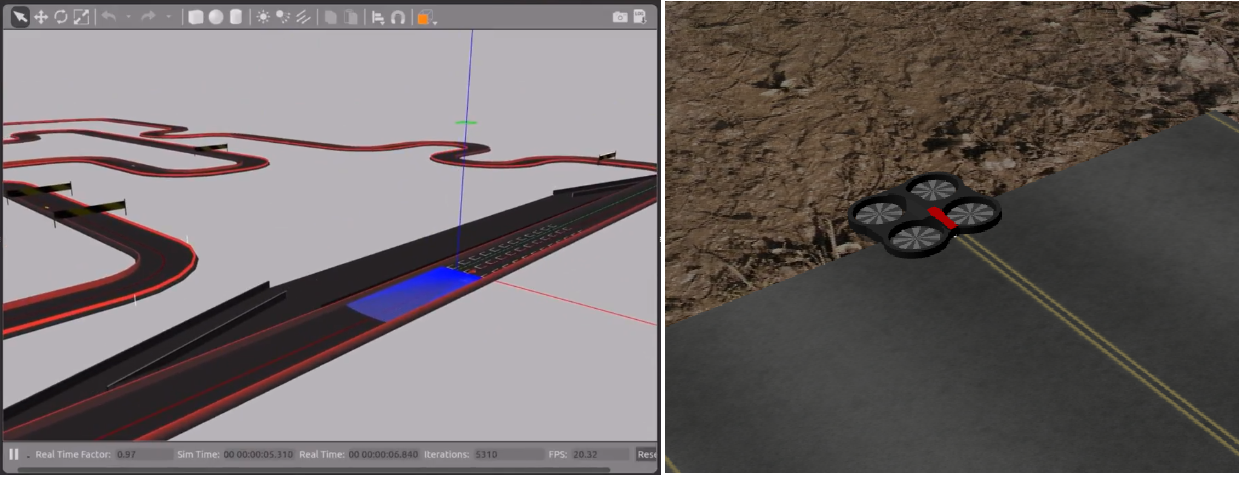
\includegraphics[width=0.9\linewidth]{figures/gazeboworlds.png}
		\caption{Visualización de la práctica XXXXX en Academy-Web}
		\label{fig.academyweb}
		\end{center}
\end{figure}


\lhead[]{CAP\'ITULO \thechapter. CHRONO}
\chapter{Ejercicio de cronometraje de vueltas competitivas con Gazebo y ROS}\label{cap.chrono}
En este capítulo del TFG ya se han definido el contexto, los objetivos y las herramientas utilizadas para la consecución de este proyecto. En este capítulo abordaremos todo lo relacionado con el desarrollo de una de las prácticas llamada \textit{Chrono}. Esta práctica forma parte del conjunto de prácticas de \textit{JdeRobot}. Se explicará la infraestructura de soporte de la práctica, el software y el funcionamiento de la práctica.

\section{Enunciado}\label{sec.enunciado}
El objetivo de esta práctica, enfocado al estudiante, es el desarrollo de un algoritmo que dote de la inteligencia necesaria a un modelo de robot F1 que compite con el récord grabado para el circuito. De esta manera, no solo se permite el desarrollo de un algoritmo funcional, sino que se propone un avance en el grado de dificultad exigiendo al alumno que optimice su algoritmo para que consiga completar una vuelta al circuito sin colisionar y con un tiempo inferior al ofrecido.

Para desarrollar la solución del algoritmo, el alumno deberá abordar distintos problemas relacionados con la programación. El primero de ellos es programar un algoritmo para realizar un filtrado de la imagen que capta el robot F1 por su cámara y escoger la línea roja central del circuito. Tras esto, el alumno deberá desarrollar un algoritmo que establezca un avance controlado del robot F1 para que siga la línea roja que ha sido filtrada por el algoritmo anterior.

Como puede observarse en los problemas abordados, además de tener que afrontar los problemas, es necesario que sean abordados conjuntamente, ya que el movimiento controlado del modelo depende del filtrado de las imágenes. Para añadir dificultad a la práctica, es necesario que el algoritmo de control de movimiento del vehículo sea eficaz dado que, de otro modo, será más lento que la solución proporcionada y llegará en segundo lugar.

\section{Infraestructura}
En esta sección se abordarán los distintos elementos involucrados en la práctica (Figura \ref{fig.infraestructura_ch}).

\begin{figure}[H]
  \begin{center}
    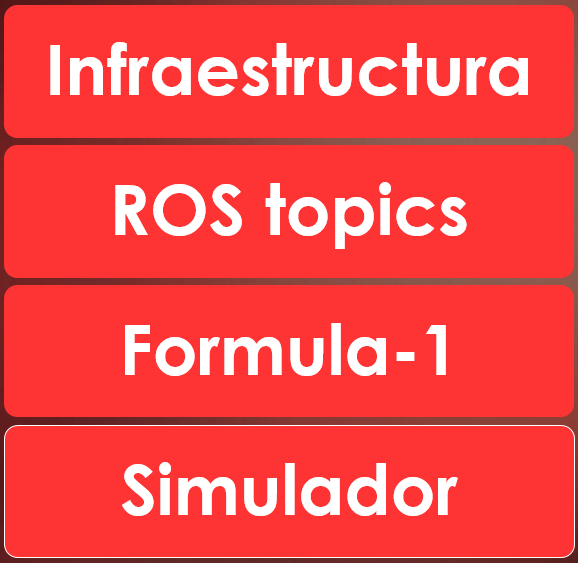
\includegraphics[width=0.4\linewidth, height=8cm]{figures/infraestructura_ch.png}
		\caption{Infraestructura de Chrono}
		\label{fig.infraestructura_ch}
		\end{center}
\end{figure}

\subsection{Modelo de robot F1}
El robot que se ha utilizado para esta práctica es un modelo de robot terrestre móvil que cuenta con 4 ruedas. El chasis elegido corresponde a un modelo de F1, específicamente del modelo RedBull. Además de este modelo se han incluido un gran conjunto de modelos de F1 correspondientes a las principales escuderías que participan en la Fórmula 1. Esto supone un total de 12 modelos de coches de escuderías reales (India, HRT, Lotus, Mclaren, Mercedes, RedBull, Renault, Tororroso, Virgin y Williams) y un modelos sin marca comercial. Además, para cada modelo de coche ha sido necesario el desarrollo de dos modelos distintos, uno que incorpora una cámara, para esta práctica, y otro modelo que tiene un láser para otras prácticas de \textit{JdeRobot}. Gracias a estos modelos, en la práctica actual puede usarse indistintamente el modelo preferido por el estudiante (Figura \ref{fig.f1s}).

\begin{figure}[H]
  \begin{center}
    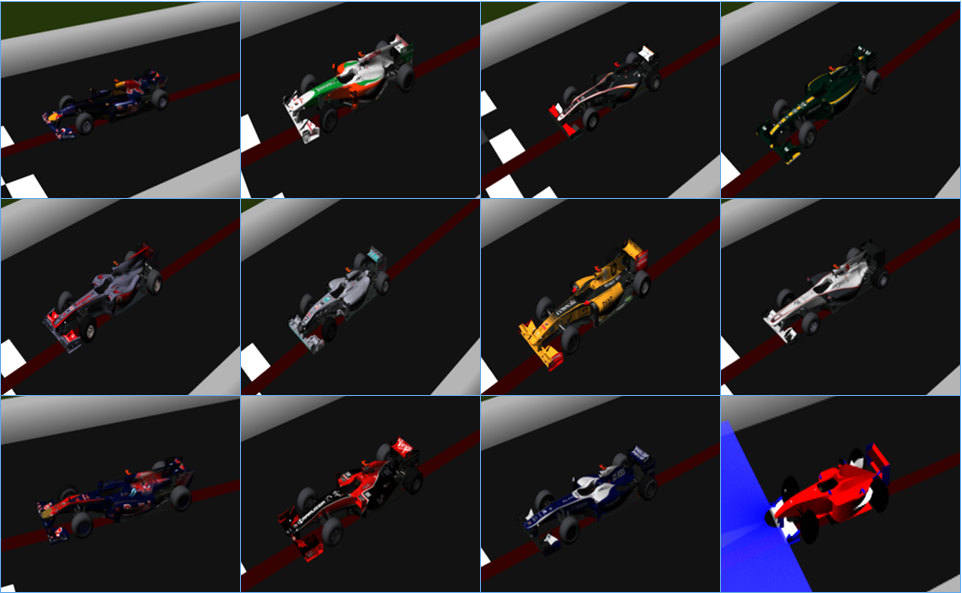
\includegraphics[width=0.99\linewidth, height=5.5cm]{figures/coches.png}
		\caption{Modelos disponibles de coches}
		\label{fig.f1s}
		\end{center}
\end{figure}

Cualquiera de los modelos de la Figura \ref{fig.f1s} utiliza los \textit{plugins} de ROS para dotar al modelo de movimiento, captación de imágenes y odometría. Estos \textit{plugins} son ofrecidos por las librerías de \textit{ROS Kinetic}:

\begin{itemize}
	\item \textit{libgazebo\_ros\_camera}
Para la captación de imágenes.
	\item \textit{libgazebo\_ros\_planar\_move}
Para el control de motores y obtener la odometría.
\end{itemize}

Tras crear el modelo, basta con importarlo en el mundo de Gazebo para su utilización.

\subsection{Cámara}
En la parte frontal del modelo se ha incluido una cámara para poder captar imágenes.

Los \textit{plugins} de la cámara dan soporte a una cámara conectada por USB con una velocidad de refresco de las imágenes de 20 fps. Gracias a esto, el modelo puede recoger imágenes a una velocidad suficiente y no perder de vista la línea. La velocidad de refresco de la cámara es un parámetro importante debido a que, dependiendo de este parámetro, entre otros, la velocidad del coche tendrá que adaptarse.

Las imágenes captadas por el \textit{plugin} son recogidas por el nodo académico que, mediante un API sencillo, proporciona las imágenes captadas y soporta la visualización de los filtros que se le apliquen a la imagen.

\subsection{Sensor Odométrico}
El sensor odométrico del modelo es imprescindible para esta práctica, ya que el nodo académico recoge la odometría del robot y la publica en un mapa con el modelo del circuito. La odometría utiliza sensores de movimiento para determinar la posición  incremental del robot con respecto a su posición inicial.

Si el robot conoce el diámetro de sus ruedas, puede conocer su posición incremental contando el número de vueltas de las mismas. El conteo de vueltas se realiza mediante \textit{encoders}, que emiten un número fijo de pulsos por revolución. En el caso de los modelos de robots F1utilizados, el refresco de la odometría se realiza a un ratio de 20. Gracias a este ratio, pueden contarse el número de vueltas y giros dados y, de esta manera, saber el recorrido realizado.

\subsection{Circuito de Nürburgring}
Para esta práctica se ha desarrollado un modelo del circuito de Nürburgring acortado. Mediante el uso de los softwares \textit{Blender} y \textit{SketchUp}, se ha modelado el circuito con una línea de salida, una grada, la carretera, paredes para evitar que el robot se salga del recorrido y césped de adorno (Figura 4.3).

\begin{figure}[H]
  \begin{center}
    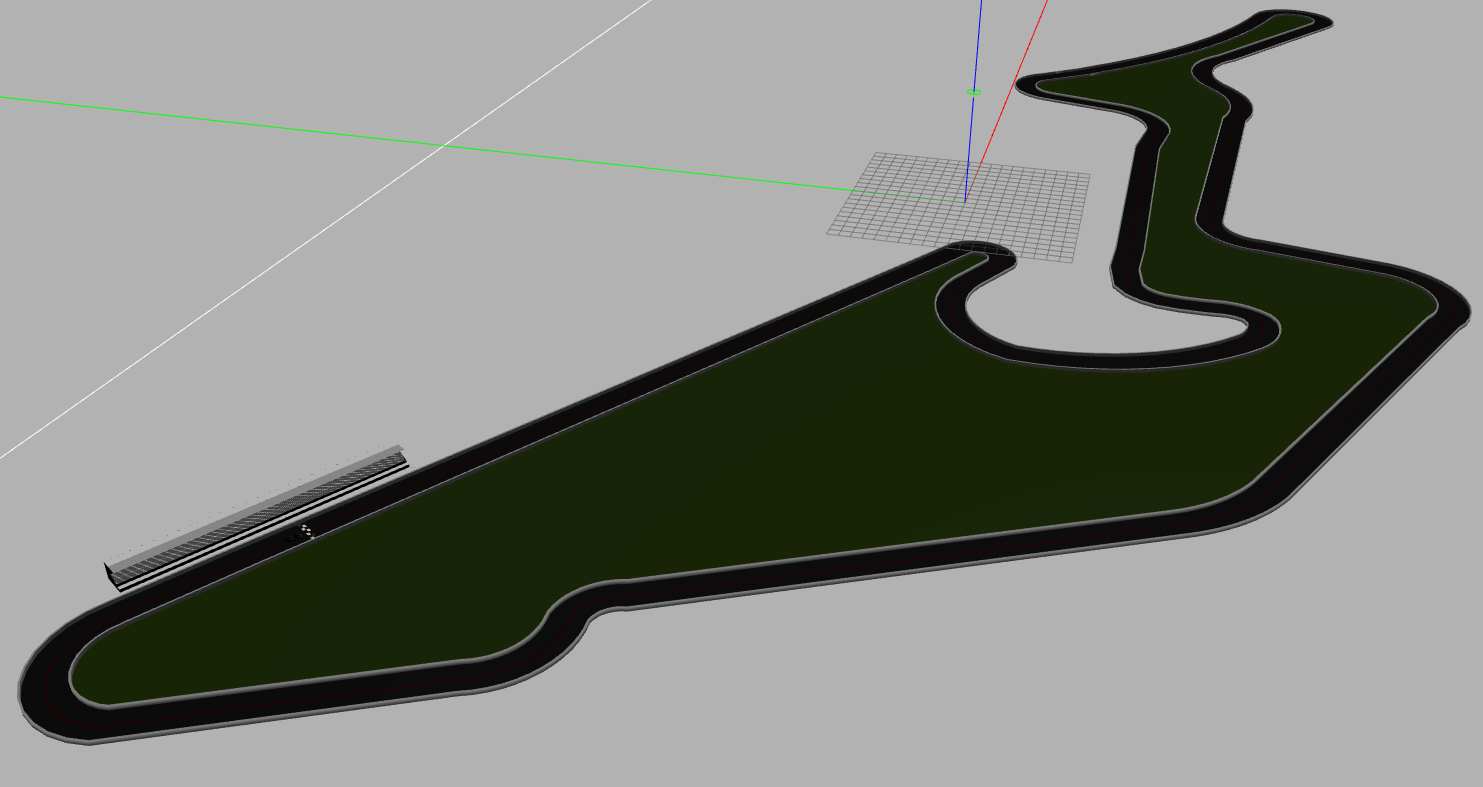
\includegraphics[width=0.95\textwidth, height=12cm]{figures/circuito.png}
		\caption{Modelo del circuito de Nürburging}
		\label{fig.circuito}
		\end{center}
\end{figure} 

\subsection{Ficheros de configuración} \label{sec.fichconf}
Para la incorporación del modelo del circuito y del robot, es necesario la creación de un modelo de configuración que importe en \textit{Gazebo} los elementos de los que consta el escenario y su localización. Este fichero tiene la extensión \textit{.world} y \textit{Gazebo} es capaz de leerlo y mostrar el escenario al iniciarse.
El código del fichero es el siguiente:

\lstset{language=XML, breaklines=true, basicstyle=\footnotesize}
\begin{lstlisting}[frame=single]
<?xml version="1.0"?>
<sdf version="1.4">
  <world name="default">
    <include>
      <uri>model://sun</uri>
    </include>
    <include>
      <uri>model://nurburgrinLine</uri>
      <pose>70 -47 0 0 0 0</pose>
    </include>
    <include>
      <uri>model://f1ROS</uri>
      <pose>0.05 -0.44 0 0 0 0.9</pose>
    </include>
  </world>
</sdf>
\end{lstlisting}

Además de este fichero de configuración, es necesario un fichero complementario que importe los \textit{plugins y drivers} de ROS-Kinetic. Este tipo de fichero tienen la extensión \textit{.launch}. En este fichero se pasan a \textit{Gazebo} argumentos como el nombre del fichero de configuración con el escenario, establecer el tiempo que se va a utilizar en el escenario, la posible implementación de un GUI y otras opciones de depuración.
El fichero es el siguiente:

\lstset{language=XML, breaklines=true, basicstyle=\footnotesize}
\begin{lstlisting}[frame=single]
<?xml version="1.0" encoding="UTF-8"?>
<launch>
  <!-- We resume the logic in empty_world.launch, changing only the name of the world to be launched -->
  <include file="$(find gazebo_ros)/launch/empty_world.launch">
    <arg name="world_name" value="nurburgrinLineROS.world"/> <!-- Note: the world_name is with respect to GAZEBO_RESOURCE_PATH environmental variable -->
    <arg name="paused" value="false"/>
    <arg name="use_sim_time" value="true"/>
    <arg name="gui" value="true"/>
    <arg name="headless" value="false"/>
    <arg name="debug" value="false"/>
    <arg name="verbose" default="false"/>
  </include>
</launch>
\end{lstlisting}

\section{Nodo Académico}
En esta sección se trata el desarrollo del nodo académico de la práctica (Figura 4.4). Este elemento ha sido desarrollado específicamente para la práctica ofreciendo al estudiante todas las herramientas necesarias para un desarrollo del algoritmo sencillo (Figura \ref{fig.na_ch}).

\begin{figure}[H]
  \begin{center}
    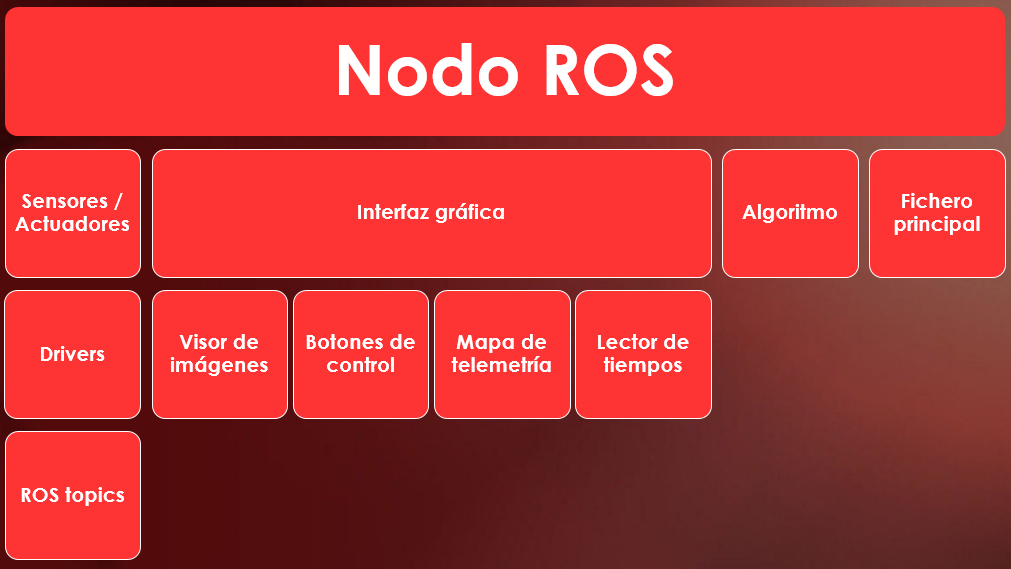
\includegraphics[width=0.5\textwidth, height=8cm]{figures/na_ch.png}
		\caption{Nodo Académico de Chrono}
		\label{fig.na_ch}
		\end{center}
\end{figure} 

\subsection{Arquitectura software}
Esta práctica tiene dos hilos de ejecución para aliviar la carga computacional de la práctica De esta manera se aumenta la velocidad  la que puede trabajar el simulador \textit{Gazebo}.

\begin{itemize}
	\item Hilo de sensores: este hilo se encarga de la actualización de los datos de los sensores del robot. Este hilo se comunica con \textit{Gazebo} para recoger datos de la odometría y la cámara y para publicar datos de control del motor para mover el robot.
	\item Hilo de la interfaz gráfica del usuario (GUI): este hilo se encarga del refresco del GUI de la práctica. En esta práctica tiene una carga computacional elevada dado se encarga de refrescar las imágenes obtenidas por la cámaras, el procesamiento visual sobre esa imagen que ha realizado el alumno, un mapa del circuito con la posición actualizada del robot y del robot fantasma a vencer, y una lectura controlada de tiempos para sincronizar ambos coches.
\end{itemize}

Gracias a esta interfaz gráfica el estudiante puede servirse de algunos elementos de depuración que veremos en profundidad en la sección 5.3.2 y 5.3.3. De esta manera el alumno solo tiene que centrarse en el desarrollo del algoritmo. El nodo académico dispone de una función reservada para que el alumno escriba su algoritmo en ella y pueda ver los resultados, todo ello viene indicado en fichero \textit{README.md} de la práctica.

\subsection{Interfaz de sensores y actuadores}
El nodo académico proporciona un API de sensores y actuadores al programador para facilitar la interconexión con los mismos. El API del robot es el siguiente:

\begin{itemize}
	\item \textit{self.pose3d.getPose3d()}: con esta función podemos obtener los datos de odometría y posición del robot.
	\item \textit{self.camera.getImage()}: con esta función se recogen las imágenes obtenidas por la cámara del robot.
	\item \textit{self.motors.senV() o self.motors.sendW()}: con esta función publicamos la velocidad y giro del robot.
\end{itemize}

\subsection{Interfaz gráfica}
La interfaz gráfica del usuario (GUI), se utiliza para representar información relacionada con los sensores del robot. Esta información es muy útil para la depuración del algoritmo del estudiante ya que permite la visualización de las publicaciones que realiza el algoritmo al robot.

Esta GUI (Figura \ref{fig.guich}) está formada por cuatro \textit{widgets}, uno para el visionado del robot, otro para su comportamiento, otro para su odometría y otro para la sincronización de la grabación de ROS con el nodo académico.

\begin{figure}[H]
  \begin{center}
    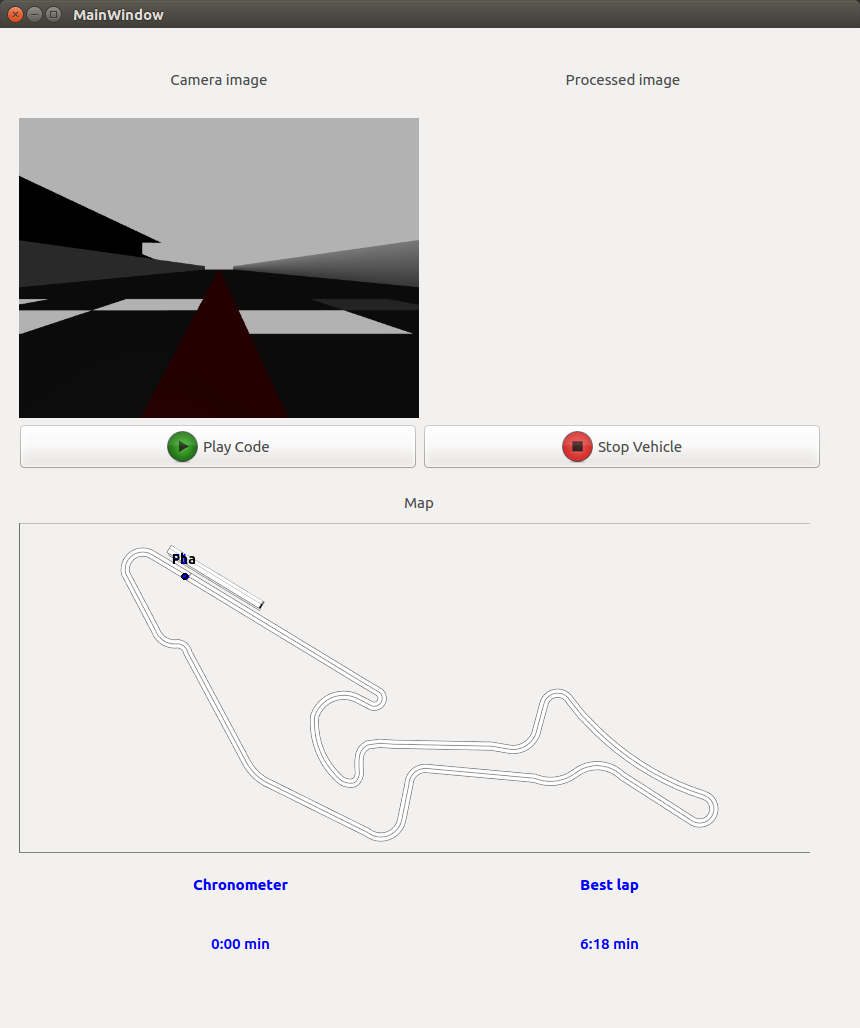
\includegraphics[width=7cm,height=10cm,\textwidth]{figures/GUI_Chrono.png}
		\caption{Interfaz Gráfica Chrono}
		\label{fig.guich}
		\end{center}
\end{figure}

El \textit{widget} superior recoge las imágenes captadas por la cámara del robot  y las muestra en una ventana del GUI. Al lado de las imágenes captadas por la cámara se muestra otra ventana con el filtrado que realice el alumno de esas imágenes. Esto es muy útil para el estudiante a la hora de enfrentarse al problema de visión que supone la primera parte de la solución de la práctica.

El tercer \textit{widget} está formado por un mapa del circuito, en este caso el circuito de Nürburgring, en el que se pueden visualizar las posiciones del robot y el robot fantasma con el récord del circuito.

El último \textit{widget} se llama \textit{ChronoWidget} y se trata de un algoritmo de de sincronización del tiempo de simulación de Gazebo con la reproducción a tiempo real de \textit{ROSbag}.

Además de estos \textit{widget}, en el GUI se incluyen distintos botones de control para hacer una pausa académica del algoritmo y para reiniciar la posición del teleoperador. El primer botón se llama \textit{pushButton} y consiste en un botón interactivo para iniciar el código programado por el alumno y para parar el código. El segundo botón se llama \textit{ResetButton} y se utiliza para reiniciar el teleoperador de la interfaz gráfica y hacer que el robot no se mueva.

La parte inferior del GUI tiene un lector de tiempos en el que se muestra el tiempo simulado de \textit{Gazebo} y, por lo tanto, el tiempo que está necesitando el robot para completar la vuelta. A su derecha se muestra el tiempo del récord del circuito para que el alumno tenga una idea de la optimización que necesita el código de control de movimiento del robot para que sea más eficiente.

\subsection{Visor de imágenes}
En este primer \textit{widget} se pueden visualizar las imágenes captadas por la cámara que incorpora el robot. Gracias a ella, el alumno puede tener una idea de la visión del robot y programar una solución de una manera más sencilla.

A la derecha de la ventana del visor de imágenes de la cámara, se ha incluido otra ventana de visualización. Esta ventana se encarga de mostrar el procesamiento de la imagen desarrollado por el alumno. Gracias a esta ventana, el alumno puede hacerse una idea del algoritmo de procesamiento de imagen que ha desarrollado.

\begin{figure}[H]
  \begin{center}
    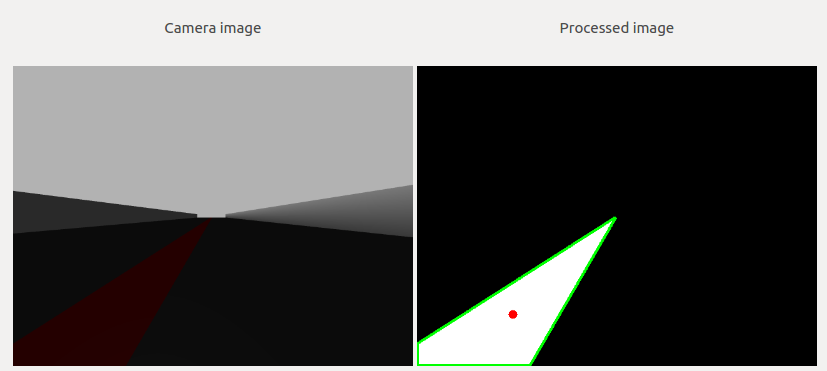
\includegraphics[width=0.98\textwidth]{figures/visor_imagen_chrono.png}
		\caption{Visor de imágenes de Chrono}
		\label{fig.vich}
		\end{center}
\end{figure}

\subsection{Botones de control}
Otra función incluida en el GUI son los botones de control. Existen dos botones de control ``Push Button''y ``Reset Button''.
Con el primer botón de control, se puede parar la ejecución de la práctica y volver a reanudarla. Con esto se permite un control en la depuración del código del alumno, ya que puede detener la ejecución en cualquier momento para visualizar los datos que seestáan recogiendo.

El segundo botón es complementario al primero, pues su funcionalidad es la de reiniciar las publicaciones de datos que se envian a los motores del robot. Es decir, con este botón se puede parar el robot y después con el botón ``Push Button'' se puede parar la ejecución.

\begin{figure}[H]
	\begin{center}
	    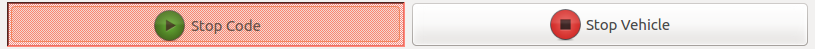
\includegraphics[width=0.98\textwidth]{figures/boton_pausa_chrono.png}
		\caption{Ilustración del botón de pausa académica}
		\label{fig.bpch}
	\end{center}
\end{figure}
\begin{figure}[H]
	\begin{center}
        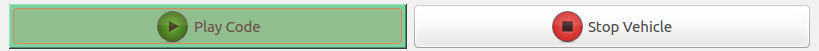
\includegraphics[width=0.98\textwidth]{figures/boton_start_chrono.png}
		\captionof{figure}{Ilustración del botón de comienzo académico}
		\label{fig.bsch}
	\end{center}
\end{figure}


\subsection{Mapa de odometría}
Ya se ha descrito la funcionalidad del mapa en la sección anterior, en esta sección nos vamos a centrar en el algoritmo que dota de esta funcionalidad al mapa.

El nodo académico, concretamente el hilo de ejecución encargado del interfaz gráfico (GUI), se encarga de cargar la imagen del mapa en el GUI. Una vez hecho esto, recoge los datos de odometría del sensor \textit{Pose3D} y dibuja su posición en el mapa. Adicionalmente, recoge los datos de odometría del fichero de grabación de ROS para extraer la posición del coche fantasma y dibujarla en el mapa también.

\begin{figure}[H]
  \begin{center}
    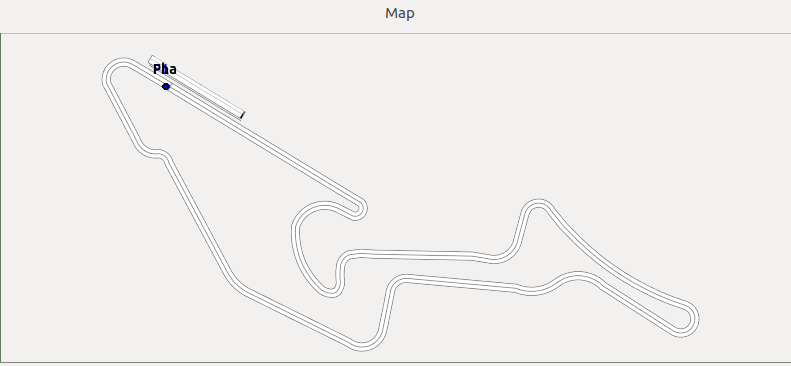
\includegraphics[width=0.98\textwidth]{figures/mapa_chrono.png}
		\caption{Mapa del GUI}
		\label{fig.mapach}
		\end{center}
\end{figure}

Esta ejecución es bastante pesada dado que requiere de una actualización constante para reflejar una posición lo más exacta posible, tanto del coche fantasma como del robot. Es por ello que se utiliza el hilo de ejecución proporcionado por el GUI. Esto alivia a la ejecución principal de una gran carga computacional.

\subsection{Lector de tiempos}
Este ha sido el principal reto de esta práctica por su complejidad a la hora de recoger los datos, tanto de \textit{Gazebo}, como de \textit{ROSbag} y sincronizarlos.

El problema que se planteaba en la sincronización de tiempos era el hecho de que los tiempos de \textit{Gazebo} se sincronizan mediante el tiempo de simulación del propio simulador pero los tiempos grabados de \textit{Gazebo} mediante ROSbag, se reproduce mediante el tiempo real. Esto supone una desincronización muy grande ya que, en el tiempo de simulación es, aproximadamente, un 0,15 veces el tiempo real. Adicionalmente existe el problema de que el tiempo de simulación depende de la potencia de cómputo de cada ordenador, por lo que la reproducción no se puede realizar a  un ritmo constante porque sería un hándicap muy grande para los ordenadores potentes que se verían afectados a reproducir de una manera muy lenta.

En este aspecto, debían abordarse los dos problemas propuestos de manera simultánea. Por un lado sincronizar el tiempo de reproducción con el tiempo de simulación, y por otro llevar un ritmo del tiempo de simulación adaptado para la carga de cómputo que pueda soportar cada ordenador. Adicionalmente se encontró un problema adicional con la reproducción de la grabación de ROSbag por el cual, las etiquetas de tiempo de las que consta, no se inicializan desde el comienzo sino que se graban con el tiempo simulado actual. Es por esto que la reproducción comienza con una etiqueta temporal distinta de cero.

Para solucionar sendos problemas ha sido necesaria la definición de diversas medidas de tiempos:

\begin{itemize}
	\item \textit{Tiempo de grabación}: este tiempo representa el ritmo al que se reproduce la grabación de ROSbag.
	\item \textit{Tiempo simulado}: este tiempo representa el tiempo al que se refresca el simulador \textit{Gazebo}.
	\item \textit{Tiempo de reproducción}: este tiempo se basa en el tiempo de simulación pero restándole el offset del comienzo de la práctica. Por ello empieza cuando el estudiante ejecuta la práctica en lugar de cuando se inicia el simulador.
\end{itemize}

El algoritmo de simulación comienza recogiendo el instante de tiempo en el que el alumno ejecuta su código mediante el comando:

\lstset{language=Python, breaklines=true, basicstyle=\footnotesize}
\begin{lstlisting}[frame=single]
initime = rospy.Time.from_sec(rospy.get_time()).to_sec()
\end{lstlisting}

Una vez obtenido el tiempo inicial, es necesario recoger el instante de tiempo en el que estamos refrescando la sincronización:

\lstset{language=Python, breaklines=true, basicstyle=\footnotesize}
\begin{lstlisting}[frame=single]
sim_time = rospy.Time.from_sec(rospy.get_time()).to_sec()
\end{lstlisting}

Además de estos dos tiempos, es necesario conocer el tiempo de la primera etiqueta de la grabación de ROSbag para comenzar a leer las etiquetas desde ese offset:
\lstset{language=Python, breaklines=true, basicstyle=\footnotesize}
\begin{lstlisting}[frame=single]
rep_start = str(bag).split('start:       ')[1].split(' ')[4].split()[0][1:-1]
\end{lstlisting}
Con el tiempo de simulación actual, el tiempo inicial y el tiempo de inicio de la reproducción, podemos obtener el tiempo con el que vamos a comparar las etiquetas temporales de la grabación para saber si tenemos que leer la etiqueta temporal y actualizar la posición del coche fantasma en el mapa del GUI o seguir devolviendo la misma posición porque es pronto.

\lstset{language=Python, breaklines=true, basicstyle=\footnotesize}
\begin{lstlisting}[frame=single]
t_sim_unif = sim_time - initime + float(rep_start)
\end{lstlisting}

Gracias a esta sincronización se pueden devolver los valores de odometría grabados para la solución con el récord de la vuelta para el coche fantasma y actualizar su posición en el mapa. A continuación se describe el código utilizado para la sincronización:

\lstset{language=Python, breaklines=true, basicstyle=\footnotesize}
\begin{lstlisting}[frame=single]
def synchronize(self):
        global posx, posy, cursor

        t_sim_unif = sim_time - initime + float(rep_start)
        if initime != 0.0 and t_sim_unif != 0.0:
            for (topic,msg,t) in bag.read_messages(start_time=rospy.Time(t_sim_unif-0.05)):
                t = t.to_sec()
                if t_sim_unif > t:
                    try:
                        posx = str(msg).split('x: ')[1].split()[0]
                        posy = str(msg).split('y: ')[1].split()[0]
                        return float(posx), float(posy)
                    except IndexError:
                        pass
                else:
                    return float(posx), float(posy)

        else:
            return float(posx), float(posy)
\end{lstlisting}

A continuación se muestra una imagen (Figura \ref{fig.ltch}) del \textit{widget} en el GUI con la práctica iniciada. A la izquierda se puede visualizar el chronómetro con la duración de la ejecución y a su derecha se encuentra el registra con el la duración de la vuelta para la grabación que se esté reproduciendo.

\begin{figure}[H]
  \begin{center}
    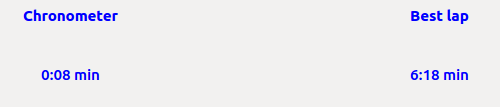
\includegraphics[width=0.98\textwidth]{figures/lector_tiempos_chrono.png}
		\caption{Lector de tiempos de Chrono}
		\label{fig.ltch}
		\end{center}
\end{figure}

\section{Soluciones de referencia}
Para la práctica, ha sido necesario el desarrollo de dos soluciones de referencia distintas. Una de ellas ha sido adaptada de una solución previamente hecha y la otra solución ha sido programada por completo.

La primera solución ha sido adaptada de otra práctica de \textit{JdeRobot Academy} llamada \textit{Follow Line}. Aunque esta práctica es similar, la solución estaba desactualizada por lo que ha sido necesaria una actualización del código, en específico de la parte de comparación de píxeles en la imagen filtrada y de la parte de control de movimiento. La actualización de la parte del control de movimiento ha sido más completa debido a que la velocidad del coche en las curvas era demasiado elevada y no estaba sincronizada con el refresco y filtrado de imagen que realiza la cámara insertada en el coche de 20 imágenes por segundo.

La segunda solución desarrollada, ha sido creada por completo utilizando la librería \textit{OpenCV}, con funciones \textit{Built-in} proporcionadas por la misma que facilitan la comprensión del código programado. Para ello ha sido necesario un estudio más profundo de esta librería que ha dotado de la inteligencia necesaria para reescribir el filtrado de imagen en un algoritmo mucho más eficiente y que permite un procesamiento de las imágenes más elevado. Gracias a esto, la velocidad del robot es mayor y por consiguiente, completa la vuelta al circuito sin colisiones y en un tiempo menor.

\subsection{Procesamiento de imagen} \label{sec.pdi}
El procesamiento de la imagen captada por la cámara, comienza con la recogida de la imagen guardada en el búffer de la misma con la instrucción:

\lstset{language=Python, breaklines=true, basicstyle=\footnotesize}
\begin{lstlisting}[frame=single]
input_image = self.camera.getImage().data
\end{lstlisting}

Gracias a esta instrucción es posible ver la imagen captada en la interfaz gráfica del usuario.

Una vez obtenida la imagen, hay que transformarla a una imagen HSV\footnote{\url{https://es.wikipedia.org/wiki/Modelo_de_color_HSV}} para poder seleccionar el color rojo de la línea central del circuito:

\lstset{language=Python, breaklines=true, basicstyle=\footnotesize}
\begin{lstlisting}[frame=single]
image_HSV = cv2.cvtColor(input_image, cv2.COLOR_RGB2HSV)
\end{lstlisting}

Tras obtener la imagen HSV, podemos seleccionar el rango de valores que componen el rojo de la línea como un array con la intensidad mínima y máxima del color.

\lstset{language=Python, breaklines=true, basicstyle=\footnotesize}
\begin{lstlisting}[frame=single]
value_min_HSV = np.array([0, 150, 0])
value_max_HSV = np.array([180, 255, 255])
\end{lstlisting}

Con esos valores realizamos un filtrado de la imagen para obtener la línea roja exclusivamente:

\lstset{language=Python, breaklines=true, basicstyle=\footnotesize}
\begin{lstlisting}[frame=single]
image_HSV_filtered = cv2.inRange(image_HSV, value_min_HSV, value_max_HSV)
\end{lstlisting}

Usamos el filtro obtenido como una máscara para filtrar la imagen y obtener de esta forma la imagen filtrada en blanc y negro. De esta manera el blanco serán los colores que pasen el filtro y en negro obtendremos el resto de colores. En este caso, obtendremos la líneaa roja del circuito en color blanco y el resto de la imagen en negro:

\lstset{language=Python, breaklines=true, basicstyle=\footnotesize}
\begin{lstlisting}[frame=single]
image_HSV_filtered_Mask = np.dstack((image_HSV_filtered, image_HSV_filtered, image_HSV_filtered))
\end{lstlisting}

Una vez filtrada la imagen, se procede a obtener los contornos de la zona filtrada. Para ello, es necesario convertir la imagen a escala de grises:

\lstset{language=Python, breaklines=true, basicstyle=\footnotesize}
\begin{lstlisting}[frame=single]
imgray = cv2.cvtColor(image_HSV_filtered_Mask, cv2.COLOR_BGR2GRAY)
\end{lstlisting}

De esta manera, se pueden conseguir los píxeles que tiene un contraste mayor con sus vecinos, obteniendo el contorno:

\lstset{language=Python, breaklines=true, basicstyle=\footnotesize}
\begin{lstlisting}[frame=single]
ret, thresh = cv2.threshold(imgray, 127, 255, 0)
_, contours, hierarchy = cv2.findContours(thresh, cv2.RETR_TREE, cv2.CHAIN_APPROX_SIMPLE)
\end{lstlisting}

Una vez conseguido el contorno, se dibuja en la imagen filtrada:

\lstset{language=Python, breaklines=true, basicstyle=\footnotesize}
\begin{lstlisting}[frame=single]
cv2.drawContours(image_HSV_filtered_Mask, contours, -1, (0,255,0), 3)
\end{lstlisting}

El siguiente algoritmo, una vez realizado el filtro, es para robustecer el código en el caso de que, en el filtrado de la imagen, se detecten dos zonas con filtro. Esto se puede producir cuando hay una curva y, debido a la resolución de la cámara, recoge la línea roja pero incompleta. Esto produce lagunas de filtro en las que no se visualiza la línea por completo, sino cortada. Para evitar un fallo en el algoritmo, ha sido necesaria la inclusión del siguiente código que recoge todas las zonas filtradas y selecciona la de mayor área:

\lstset{language=Python, breaklines=true, basicstyle=\footnotesize}
\begin{lstlisting}[frame=single]
area = []
for pic, contour in enumerate(contours):
    area.append(cv2.contourArea(contour))
if len(area) > 1:
    if area[0] < area[1]:
        M = cv2.moments(contours[1])
    else:
        M = cv2.moments(contours[0])
else:
    M = cv2.moments(contours[0])
\end{lstlisting}

Tras esta comprobación, se obtienen los valores de los ejxes x e y de la zona filtrada. Estos valores forman el centro del área que ha sido filtrada:

\lstset{language=Python, breaklines=true, basicstyle=\footnotesize}
\begin{lstlisting}[frame=single]
if int(M['m00']) != 0:
    self.cx = int(M['m10']/M['m00'])
    self.cy = int(M['m01']/M['m00'])
\end{lstlisting}

Gracias a estos valores, en concreto al valor del eje x, podemos saber la diferencia de posición que tiene el robot con el centro de la línea roja, es decir, la diferencia de posición del robot con el centro del circuito. Para facilitar este cálculo, se ha dibujado un punto en la imagen filtrada con los valores del eje y el eje y para que sea visualizado:

\lstset{language=Python, breaklines=true, basicstyle=\footnotesize}
\begin{lstlisting}[frame=single]
cv2.circle(image_HSV_filtered_Mask, (self.cx, self.cy), 7, np.array([255, 0, 0]), -1)
\end{lstlisting}

Para la visualización de la imagen procesada, basta con utilizar la instrucción proporcionada por la interfaz gráfica del usuario:

\lstset{language=Python, breaklines=true, basicstyle=\footnotesize}
\begin{lstlisting}[frame=single]
self.setImageFiltered(image_HSV_filtered_Mask)
\end{lstlisting}

\subsection{Control de movimiento}
En esta sección vamos a tratar el control del movimiento del robot. Es una parte compleja ya que supone un filtrado correcto. En caso contrario, el comportamiento del movimiento del robot será incorrecto. Esto es debido a que el movimiento del robot se realiza en consecuencia al procesamiento de la imagen.

\subsubsection{Filtrado de imagen y control de movimiento basado en píxeles} \label{subsec.ficmbp}
Este tipo de control de movimiento se basa en la primera solución de la práctica y supone una transformación de la imagen a blanco y negro, para después comprobar los píxeles que cambian de tono para saber hacia qué lado hay que orientar al coche.
Se trata de una solución eficaz aunque poco eficiente. Esto es debido a que es necesario comprobar los píxeles uno a uno para averiguar qué píxeles son los que han sufrido esta transformación de tono:

\lstset{language=Python, breaklines=true, basicstyle=\footnotesize}
\begin{lstlisting}[frame=single]
# Shape gives us the number of rows and columns of an image
size = image.shape
rows = size[0]
columns = size[1]

#  Looking for pixels that change of tone
position_pixel_left = []
position_pixel_right  = []

for i in range(0, columns-1):
    value = image_HSV_filtered[365, i] - image_HSV_filtered[365, i-1]
    if(value != 0):
        if (value == 255):
            position_pixel_left.append(i)
        else:
            position_pixel_right.append(i-1)


# Calculating the intermediate position of the road
if ((len(position_pixel_left) != 0) and (len(position_pixel_right) != 0)):
    position_middle = (position_pixel_left[0] + position_pixel_right[0]) / 2
elif ((len(position_pixel_left) != 0) and (len(position_pixel_right) == 0)):
    position_middle = (position_pixel_left[0] + columns) / 2
elif ((len(position_pixel_left) == 0) and (len(position_pixel_right) != 0)):
    position_middle = (0 + position_pixel_right[0]) / 2
else:
    position_pixel_right.append(1000)
    position_pixel_left.append(1000)
    position_middle = (position_pixel_left[0] + position_pixel_right[0])/ 2

# Calculating the desviation
desviation = position_middle - (columns/2)
\end{lstlisting}

Una vez obtenidos estos píxeles, el control de movimiento se ejecuta según el siguiente algoritmo, que comprueba estos píxeles y se mueve en consecuencia:

\lstset{language=Python, breaklines=true, basicstyle=\footnotesize}
\begin{lstlisting}[frame=single]
if (desviation == 0):
     self.motors.sendV(3)
elif (position_pixel_right[0] == 1000):
     self.motors.sendW(-0.0000035)
elif ((abs(desviation)) < 85):
     if ((abs(desviation)) < 31):
         self.motors.sendV(3)
     else:
         self.motors.sendV(1)
     self.motors.sendW(-0.000045 * desviation)
elif ((abs(desviation)) < 150):
     if ((abs(desviation)) < 120):
         self.motors.sendV(1)
     else:
         self.motors.sendV(1)
     self.motors.sendW(-0.00045 * desviation)
else:
     self.motors.sendV(1)
     self.motors.sendW(-0.0055 * desviation)
\end{lstlisting}

\subsubsection{Filtrado de imagen y control de movimiento basado en el centro del contorno}
Este tipo de filtrado de imagen es el descrito en la sección \ref{sec.pdi} y es mucho más eficiente y con una eficacia mayor que el descrito en el apartado anterior\ref{subsec.ficmbp}. Esto es debido a que no necesita comprobar la imagen completa píxel a píxel, sino que filtra el área de la línea y procesa su centro.

Una vez hecho este filtro, la control de movimiento es sencillo, pues basta con obtener el valor del eje x cuando el coche está alineado con la línea recta y tomarlo como el movimiento nulo. Tras esto, se puede definir el giro del robot en consonancia con este valor de movimiento nulo.
Gracias a ello, el robot girará más o menos cuanto mayor sea la diferencia entre el valor de movimiento nulo (153 aproximadamente) y el valor actual del eje x:

\lstset{language=Python, breaklines=true, basicstyle=\footnotesize}
\begin{lstlisting}[frame=single]
if self.cx < 50:
    self.motors.sendV(1.5)
else:
    self.motors.sendV(3.5)

self.motors.sendW((153-int(self.cx))*0.01)
\end{lstlisting}

\section{Experimentación}
La optimización de los algoritmos anteriores ha sido posible gracias a la realización de diversos experimentos. Estos experimentos han hecho salir a la luz errores en el algoritmo desarrollado que han sido subsanados.

Además se han realizado experimentos globales donde se ha testeado la práctica en su totalidad, nodo académico, infraestructura de la práctica y solución desarrollada.

\subsection{Ejecución típica}
Se ha preparado un documento \textit{README.md}, incluido en la infraestructura de la práctica, que sirve de guía al alumno a la hora de ejecutar la práctica. En él se incluye información acerca de su ejecución, la API de los sensores y actuadores de ROS e, incluso, un vídeo demostrativo con una ejecución.

Para ejecutar al práctica, es necesario lanzar en una terminal el fichero de configuración de ROS, llamado \textit{f1-chrono.launch}, descrito en la sección \ref{sec.fichconf}. Para lanzar el fichero hay que ejecutar el siguiente comando:

\lstset{language=bash, breaklines=true, basicstyle=\footnotesize}
\begin{lstlisting}[frame=single]
roslaunch f1-chrono.launch
\end{lstlisting}

Una vez lanzado el comando en la terminal, se abrirá el simulador \textit{Gazebo} con el escenario del circuito (Figura \ref{fig.circuito}).

\begin{figure}[H]
  \begin{center}
    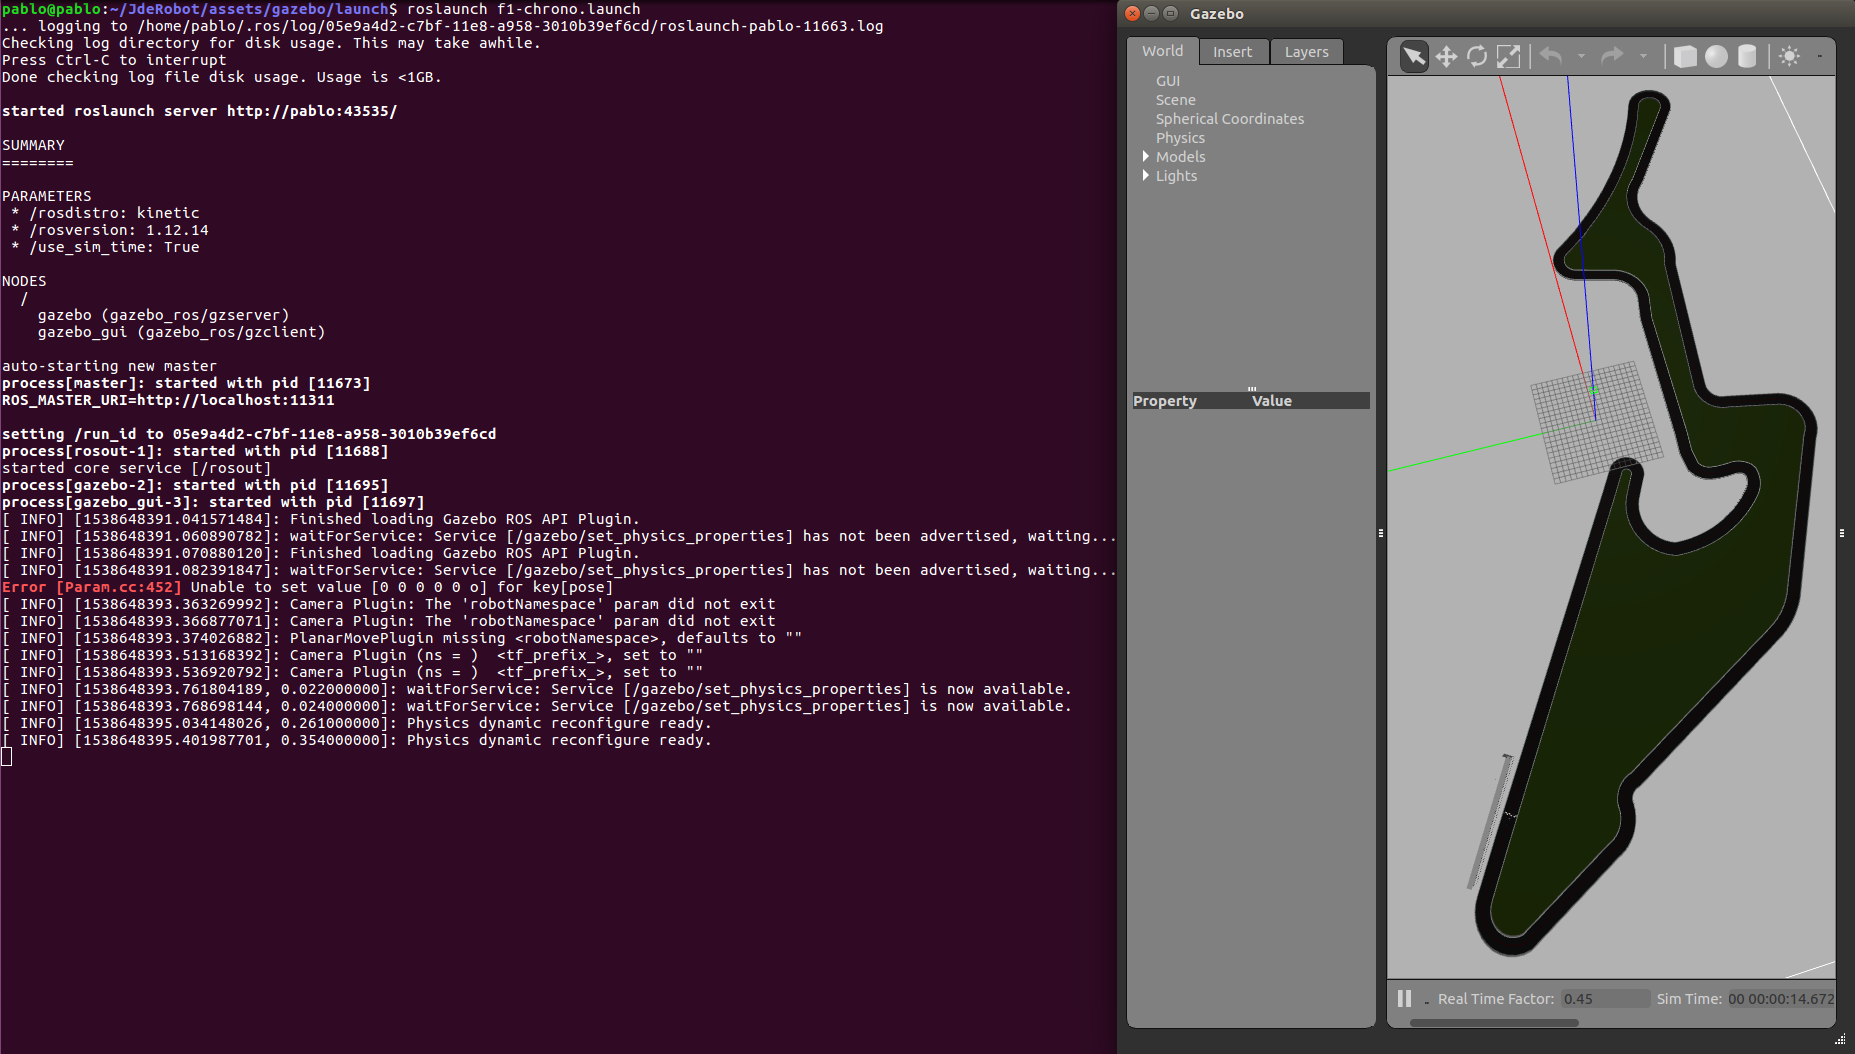
\includegraphics[width=0.98\textwidth]{figures/roslaunch_chrono.png}
		\caption{Inicialización ROS y Gazebo}
		\label{fig.roslaunchch}
		\end{center}
\end{figure}

Para iniciar el componente académico, será necesario ejecutar otro comando en una terminal distinta:

\lstset{language=bash, breaklines=true, basicstyle=\footnotesize}
\begin{lstlisting}[frame=single]
cd ~/Academy/exercises/chrono
python2 chrono.py
\end{lstlisting}

Una vez ejecutado el comando, el componente académico enlazará los sensores y actuadores proporcionados por \textit{ROS-Kinetic} mediante el fichero de configuración lanzado previamente a las variables:

\begin{itemize}
    \item self.camera
    \item self.pose3d
    \item self.motors
\end{itemize}

Con estas variables, el nodo académico se comunica con los \textit{drivers} de \textit{ROS-Kinetic}.
Además de realizar la conexión con los sensores y actuadores, al ejecutar la instrucción, nos aparecerá la interfaz gráfica de usuario (GUI) en la que se podrá visualizar las imágenes recogidas por la cámara, los botones de control, el mapa del circuito y el lector de tiempos (Figura \ref{fig.inaGch}).

\begin{figure}[H]
  \begin{center}
    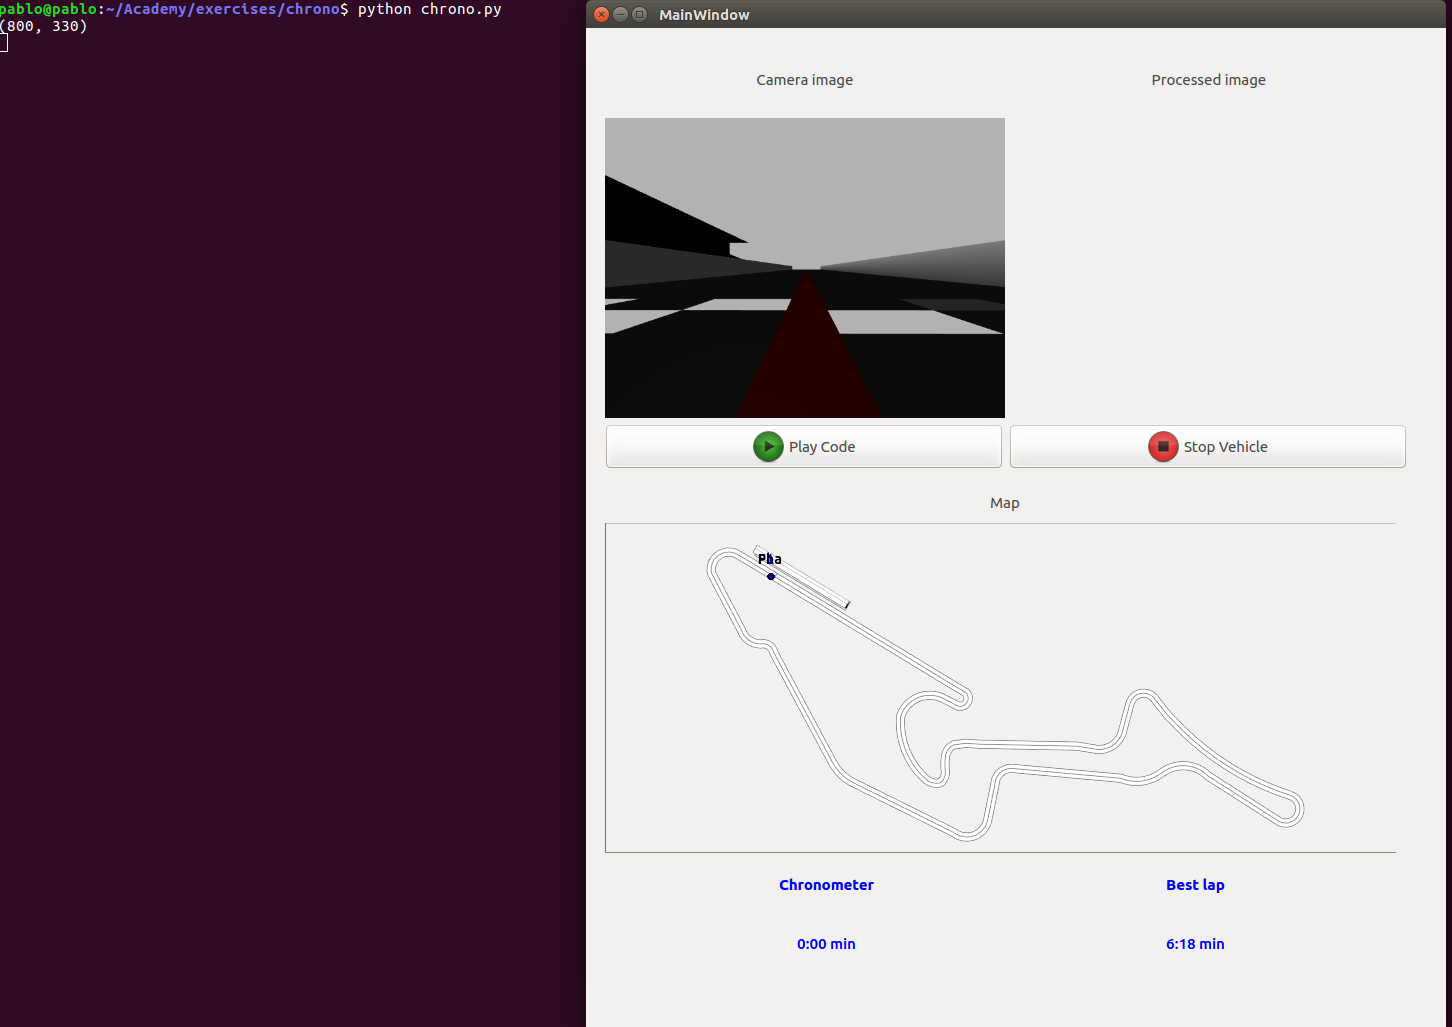
\includegraphics[width=0.98\textwidth]{figures/init_na_chrono.png}
		\caption{Inicialización del nodo académico y el GUI}
		\label{fig.inaGch}
		\end{center}
\end{figure}

Una vez inicializados los \textit{drivers de ROS-Kinetic}, el escenario en el simulador y el nodo académico, con su GUI, se puede iniciar el algoritmo desarrollado por el alumno pulsando sobre el botón ``Play Code''. De esta manera, la lógica programada podrá ser visualizada tanto en el GUI, como en el simulador.
 
\subsection{Ejecución estática}
En el caso en el que el alumno no programe el control de movimiento en su algoritmo, es posible ejecutar el código de igual manera. Esto es útil para depurar el algoritmo de procesamiento de imagen. 

El alumno tiene dos opciones en este aspecto. La primera consiste en dejar el robot inmóvil y ver el procesamiento realizado en la ventana para la imagen procesada del GUI. 

\begin{figure}[H]
  \begin{center}
    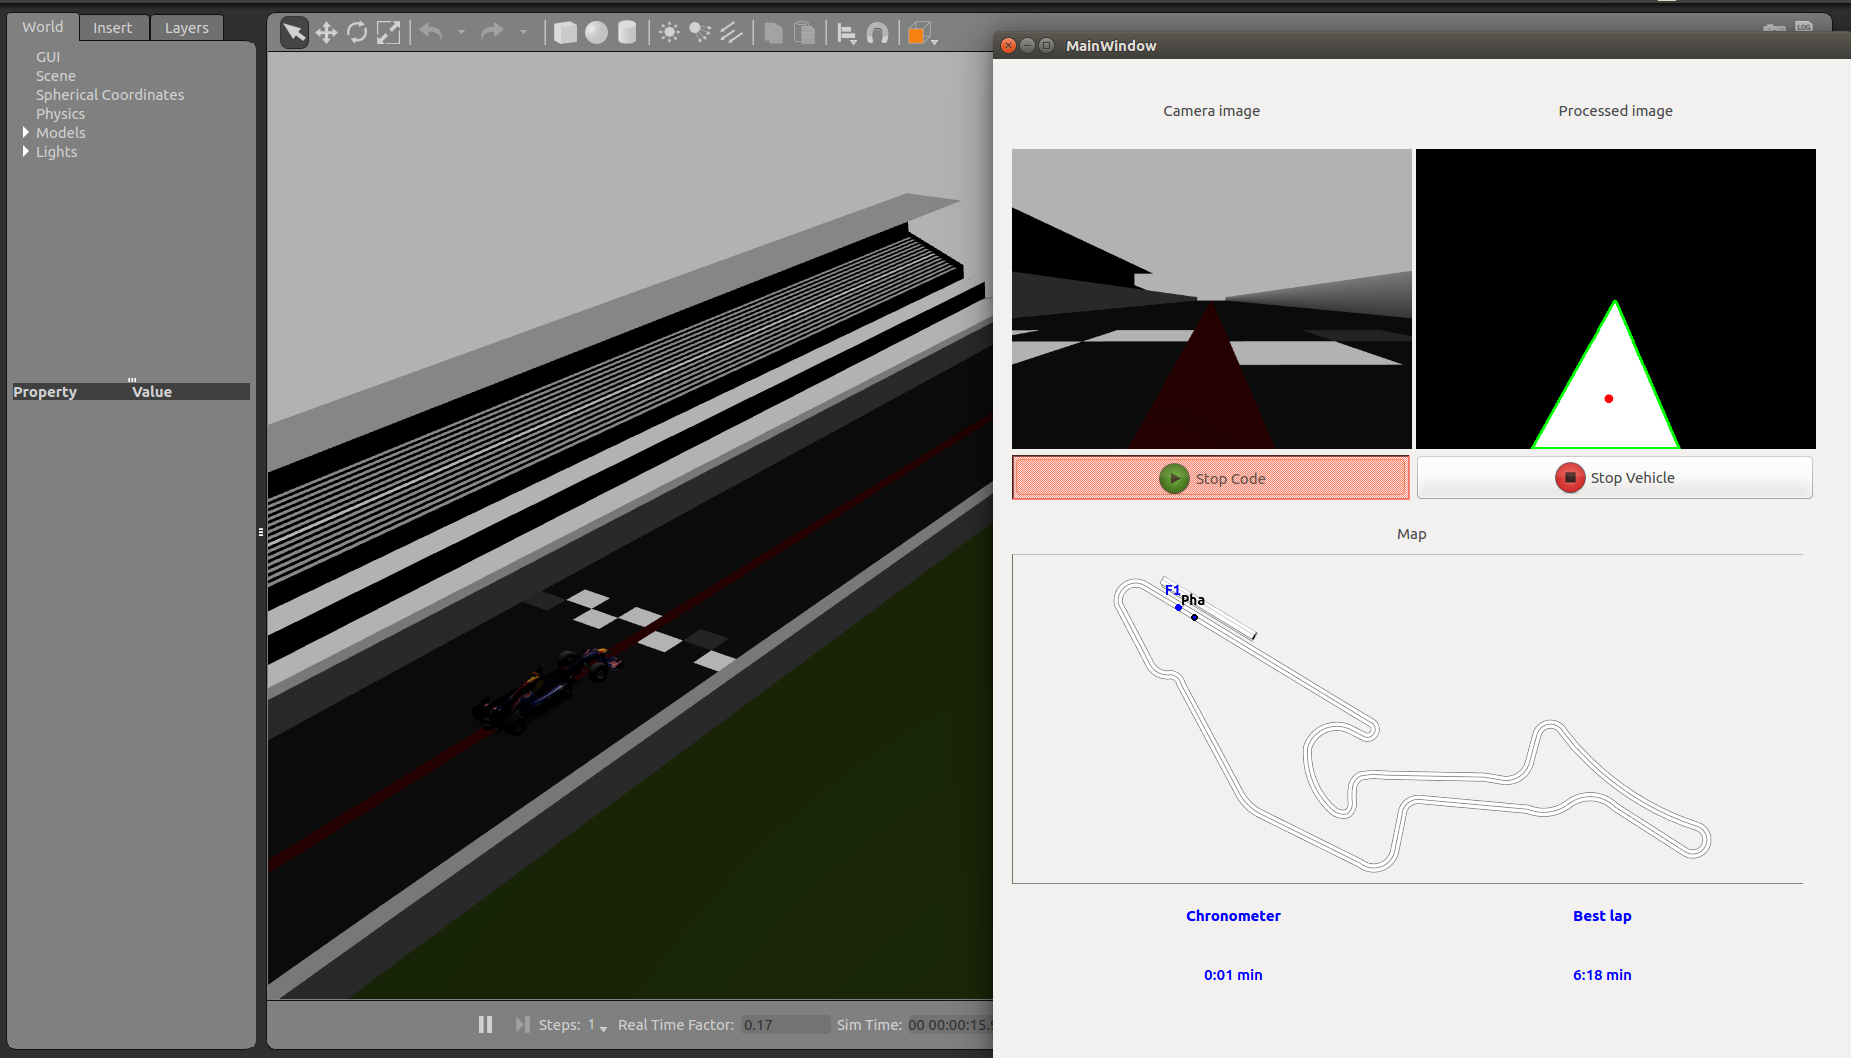
\includegraphics[width=0.98\textwidth]{figures/ejec_estat_chrono.png}
		\caption{Ejecución estática de la práctica}
		\label{fig.eech}
		\end{center}
\end{figure}

Otra opción, una vez haya superado esa primera prueba, es seleccionar una velocidad fija para mover el robot y visualizar el filtrado en movimiento.

\lstset{language=Python, breaklines=true, basicstyle=\footnotesize}
\begin{lstlisting}[frame=single]
self.motors.sendV(1)
\end{lstlisting}

\begin{figure}[H]
  \begin{center}
    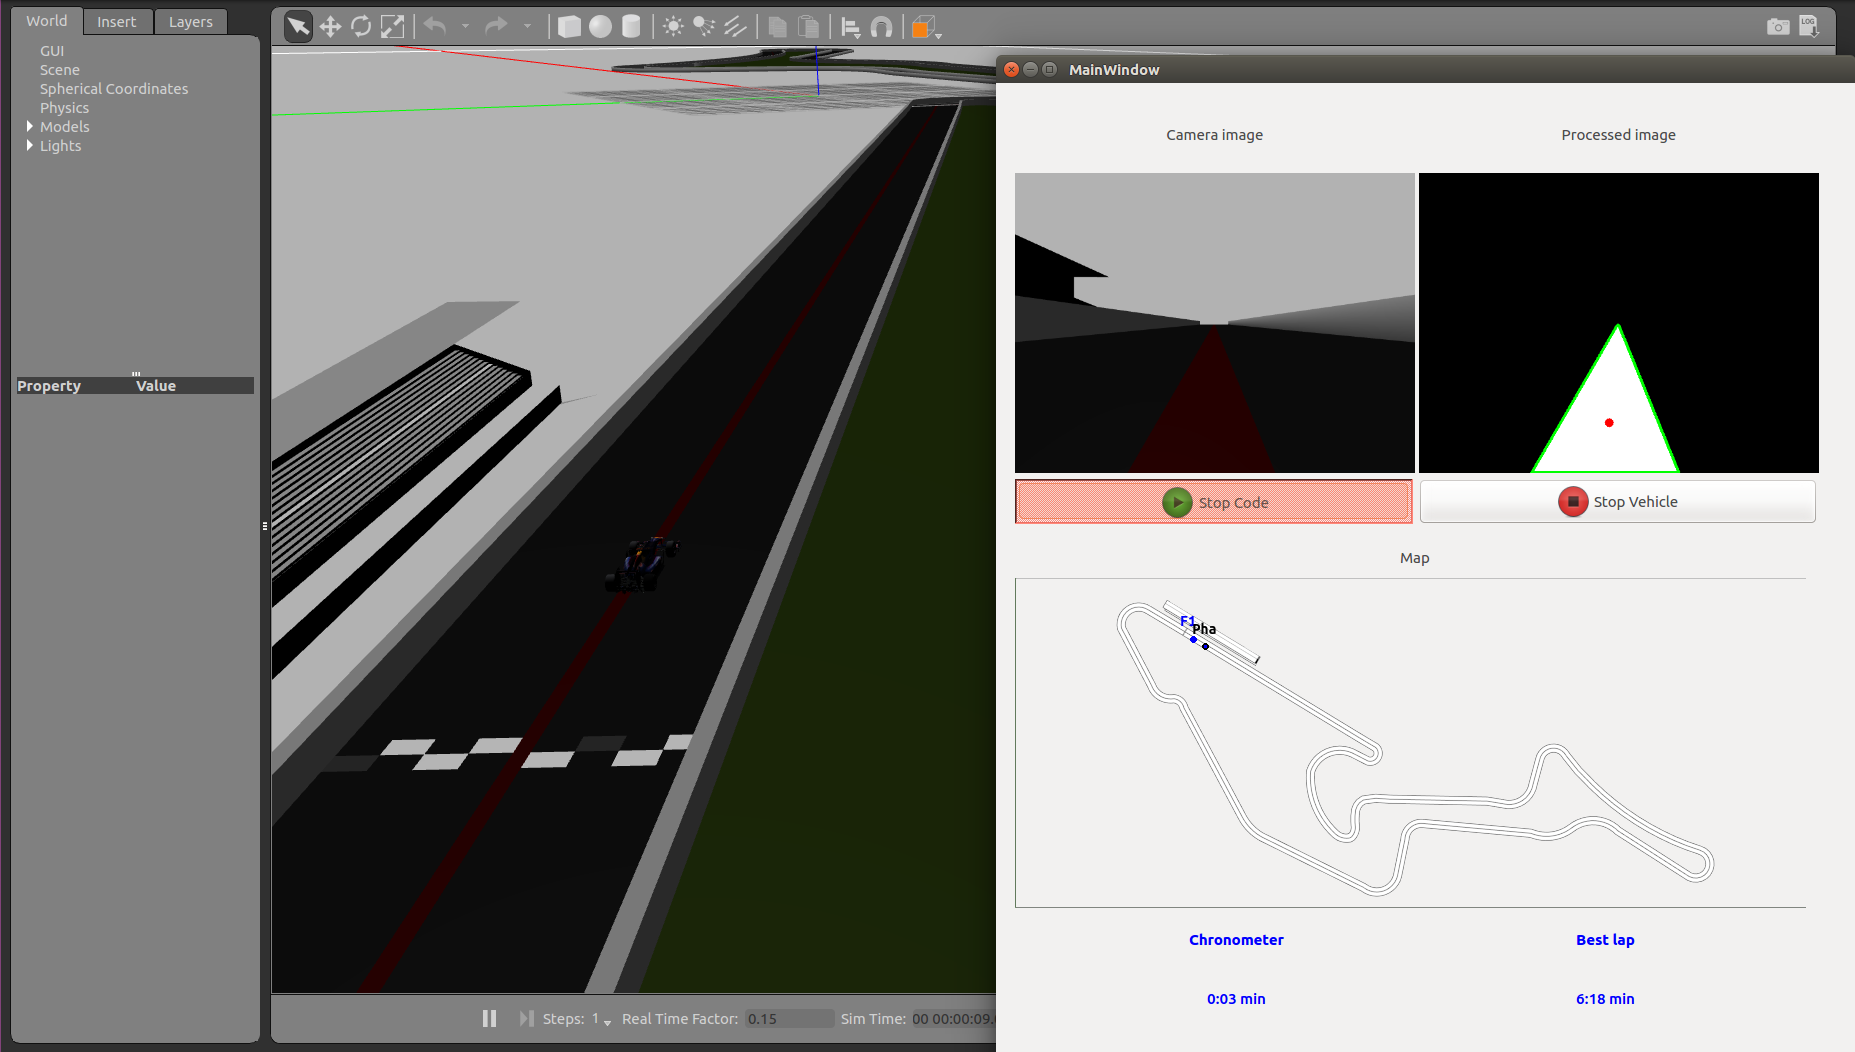
\includegraphics[width=0.98\textwidth]{figures/ejec_semiestat_chrono.png}
		\caption{Ejecución con velocidad fija}
		\label{fig.esech}
		\end{center}
\end{figure}

Con esta ejecución semi-móvil de la práctica, el alumno también puede visualizar, no solo la odometría del fantasma, que se visualizará cada vez que se ejecute el algoritmo, sino la odometría del robot a programar. Con esto, el alumno se puede hacer una idea de la velocidad a la que tiene que programar el control de movimiento para ser más veloz que el récord del circuito.

\begin{figure}[H]
  \begin{center}
    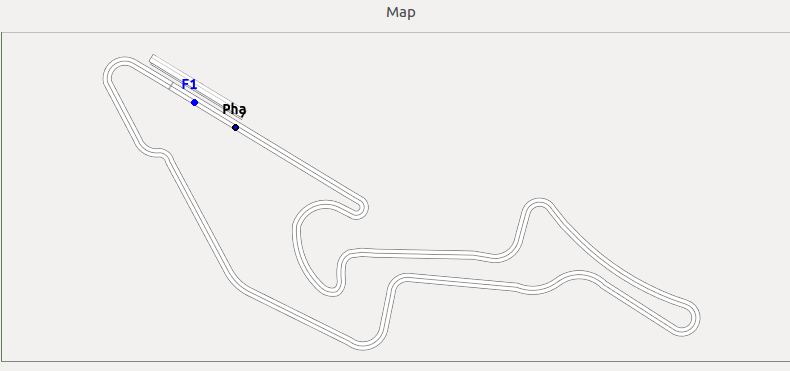
\includegraphics[width=0.98\textwidth]{figures/odom_semiestat_chrono.png}
		\caption{Odometría en ejecución con teleoperador}
		\label{fig.oet}
		\end{center}
\end{figure}

\subsection{Ejecución en movimiento}
Una vez conseguido un algoritmo que procese las imágenes en movimiento con el teleoperador, el alumno puede pasar a la última fase del desarrollo de la solución, el control de movimiento del robot. Para ello deberá utilizar el procesamiento de la imagen realizado en la primera parte del desarrollo del algoritmo para poder dotar al robot de un movimiento en función del filtrado que realice de la línea roja del circuito.
En este punto hay que tener especial cuidado con las curvas dado que la línea varía bruscamente y, con una velocidad elevada, la línea puede salirse del rango de captura de imagen de la cámara y, por lo tanto, el algoritmo producirá un error (a menos que se programe una solución para ese caso). Es por esto que el alumno debe ser consciente de la velocidad de refresco de la imagen de la cámara, 20 frames por segundo, y de la velocidad con la que el nodo recoge las imágenes de la cámara. Esta última función es la más limitante en cuanto a refresco en el procesamiento de la imagen, dado que, aunque utiliza una hebra para la interconexión entre los sensores y actuadores con el nodo académico. Debido a la odometría y a la sincronización, el hilo de ejecución no recoge las 20 imágenes por segundo que capta la cámara sino que dependerá de la potencia computacional de cada ordenador.

\begin{figure}[H]
  \begin{center}
    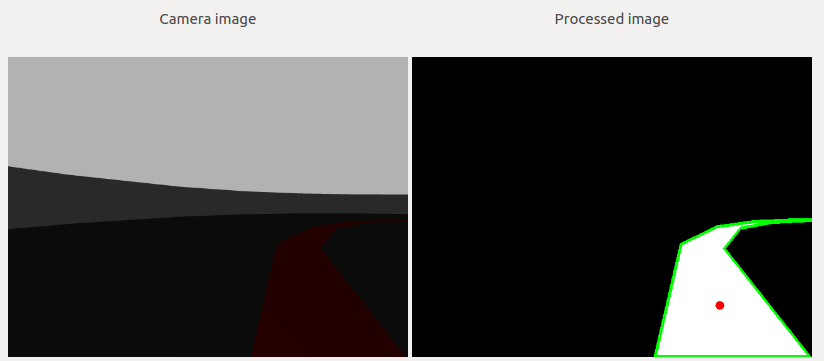
\includegraphics[width=0.98\textwidth]{figures/filtrado_curvas_chrono.png}
		\caption{Ejemplo de procesamiento de la imagen en las curvas}
		\label{fig.pdiecch}
		\end{center}
\end{figure}

Por último, una vez que se ha desarrollado el algoritmo completo, se puede ejecutar la práctica con el algoritmo.

\begin{figure}[H]
  \begin{center}
    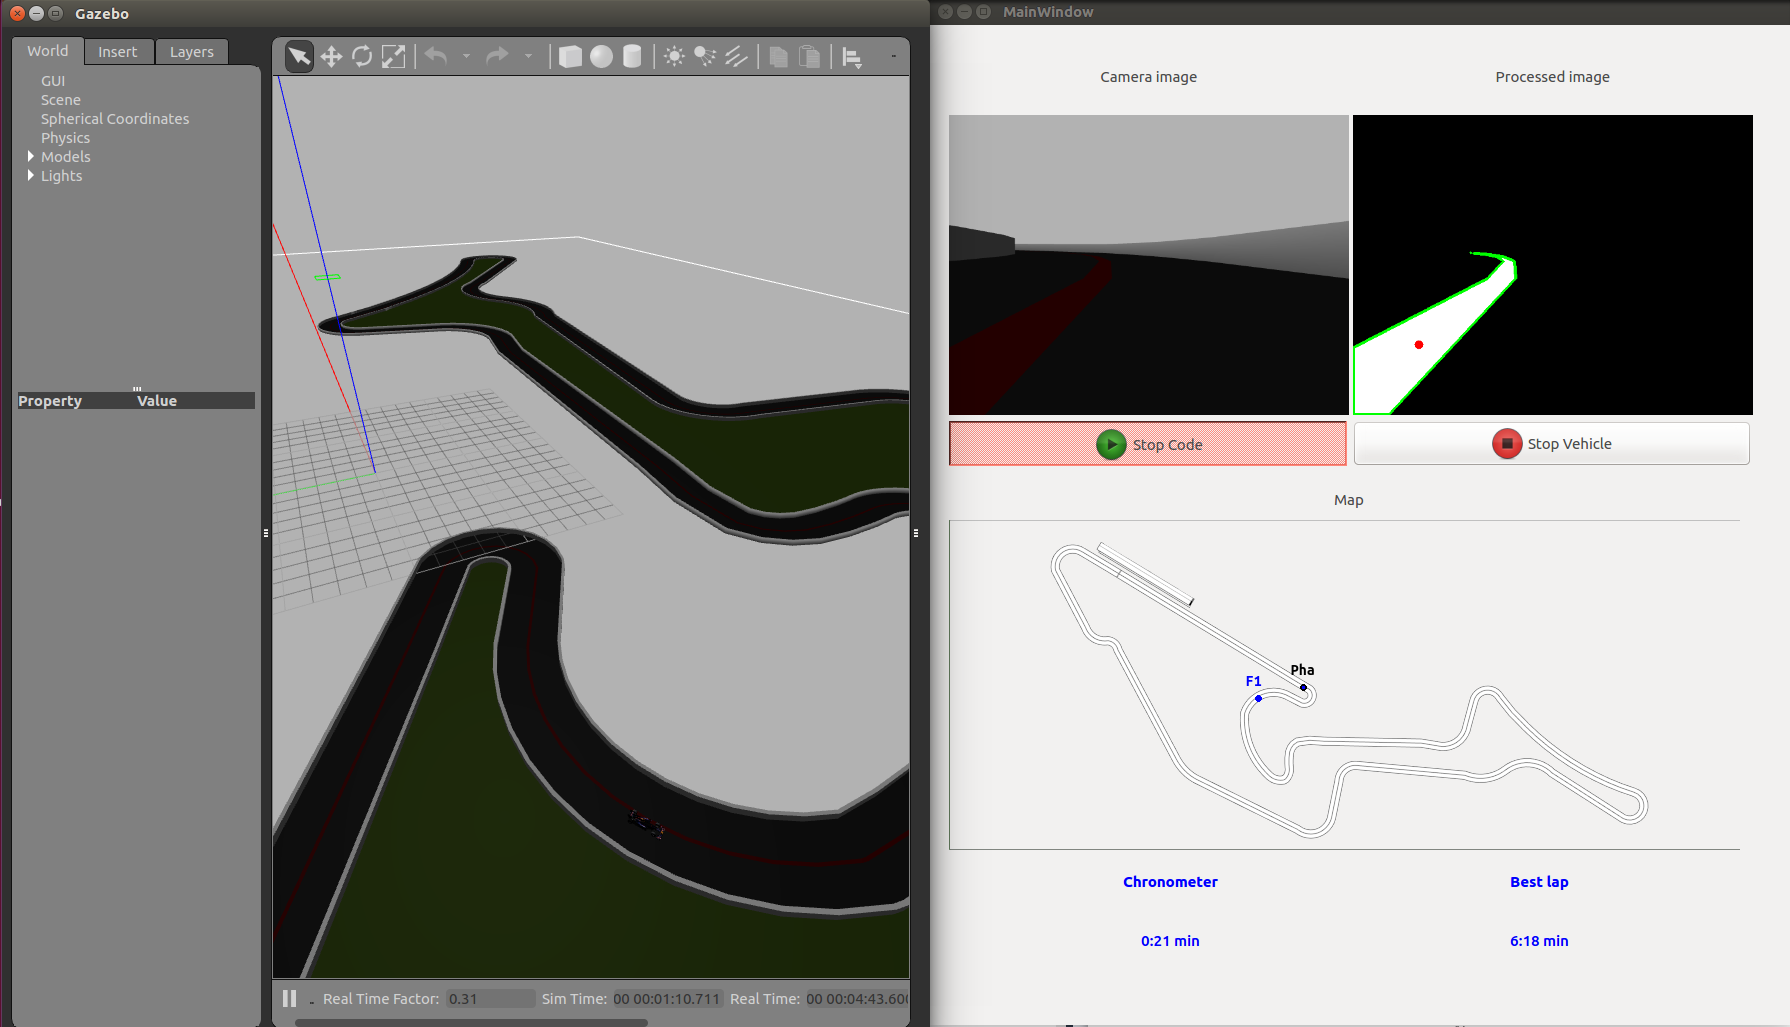
\includegraphics[width=0.98\textwidth]{figures/ejec_algoritmo_ch.png}
		\caption{Ejecución con la solución}
		\label{fig.ealgch}
		\end{center}
\end{figure}

\section{Cuadernillo académico Jupyter}
Como parte paralela a la práctica incluida en \textit{JdeRobot-Academy}, se ha desarrollado la misma práctica en con cuadernillos de \textit{Jupyter}. Gracias a esto, el alumno puede programar y ejecutar el código mediante la utilización del navegador web que prefiera.

Esto supone un paso importante hacia la multiplataforma del entorno docente \textit{JdeRobot Academy}, dado que el alumno puede acceder a las prácticas desde el sistema operativo que prefiera, pues sólo necesita acceso a internet.

Para que sea posible este hecho, ha sido necesaria una reestructuración del nodo académico y de los ficheros que lo componen, además del método de desarrollo del algoritmo.

En primer lugar. el nodo académico tiene la siguiente estructura:

\begin{figure}[H]
  \begin{center}
    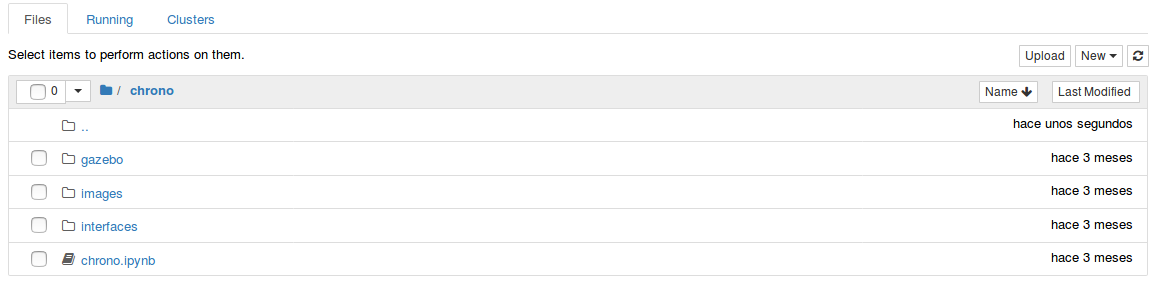
\includegraphics[width=0.98\textwidth]{figures/estructura_jupyter.png}
		\caption{Estructura de la práctica en Jupyter}
		\label{fig.ejch}
		\end{center}
\end{figure}

Como puede verse es diferente a la estructura presente en \textit{JdeRobot-Academy}. Ahora se divide en los siguiente fichero y carpetas:

\begin{itemize}
    \item images: en este directorio aparecen las imágenes contenidas en el cuadernillo.
    \item gazebo: en este directorio está el fichero de configuración con el escenario y con los \textit{drivers} de \textit{ROS-Kinetic}.
    \item interfaces: en este directorio se encuentran los \textit{drivers} de \textit{ROS-Kinetic}.
    \item chrono.ipynb: este fichero es el cuadernillo ejecutable en Jupyter.
\end{itemize}

Para acceder a la práctica, el alumno debe iniciar Jupyter introduciendo en la terminal el siguiente comando:

\lstset{language=bash, breaklines=true, basicstyle=\footnotesize}
\begin{lstlisting}[frame=single]
cd ~/Jupyter
jupyter-notebook
\end{lstlisting}

Con esto se abrirá el navegador web por defecto en la carpeta local Jupyter. Una vez hecho esto, navegaremos hacia el directorio de la práctica de Jupyter ``Chrono'' y abriremos el fichero ``Chrono.ipynb''. Tras esto se mostrará la siguiente imagen del cuadernillo:

\begin{figure}[H]
  \begin{center}
    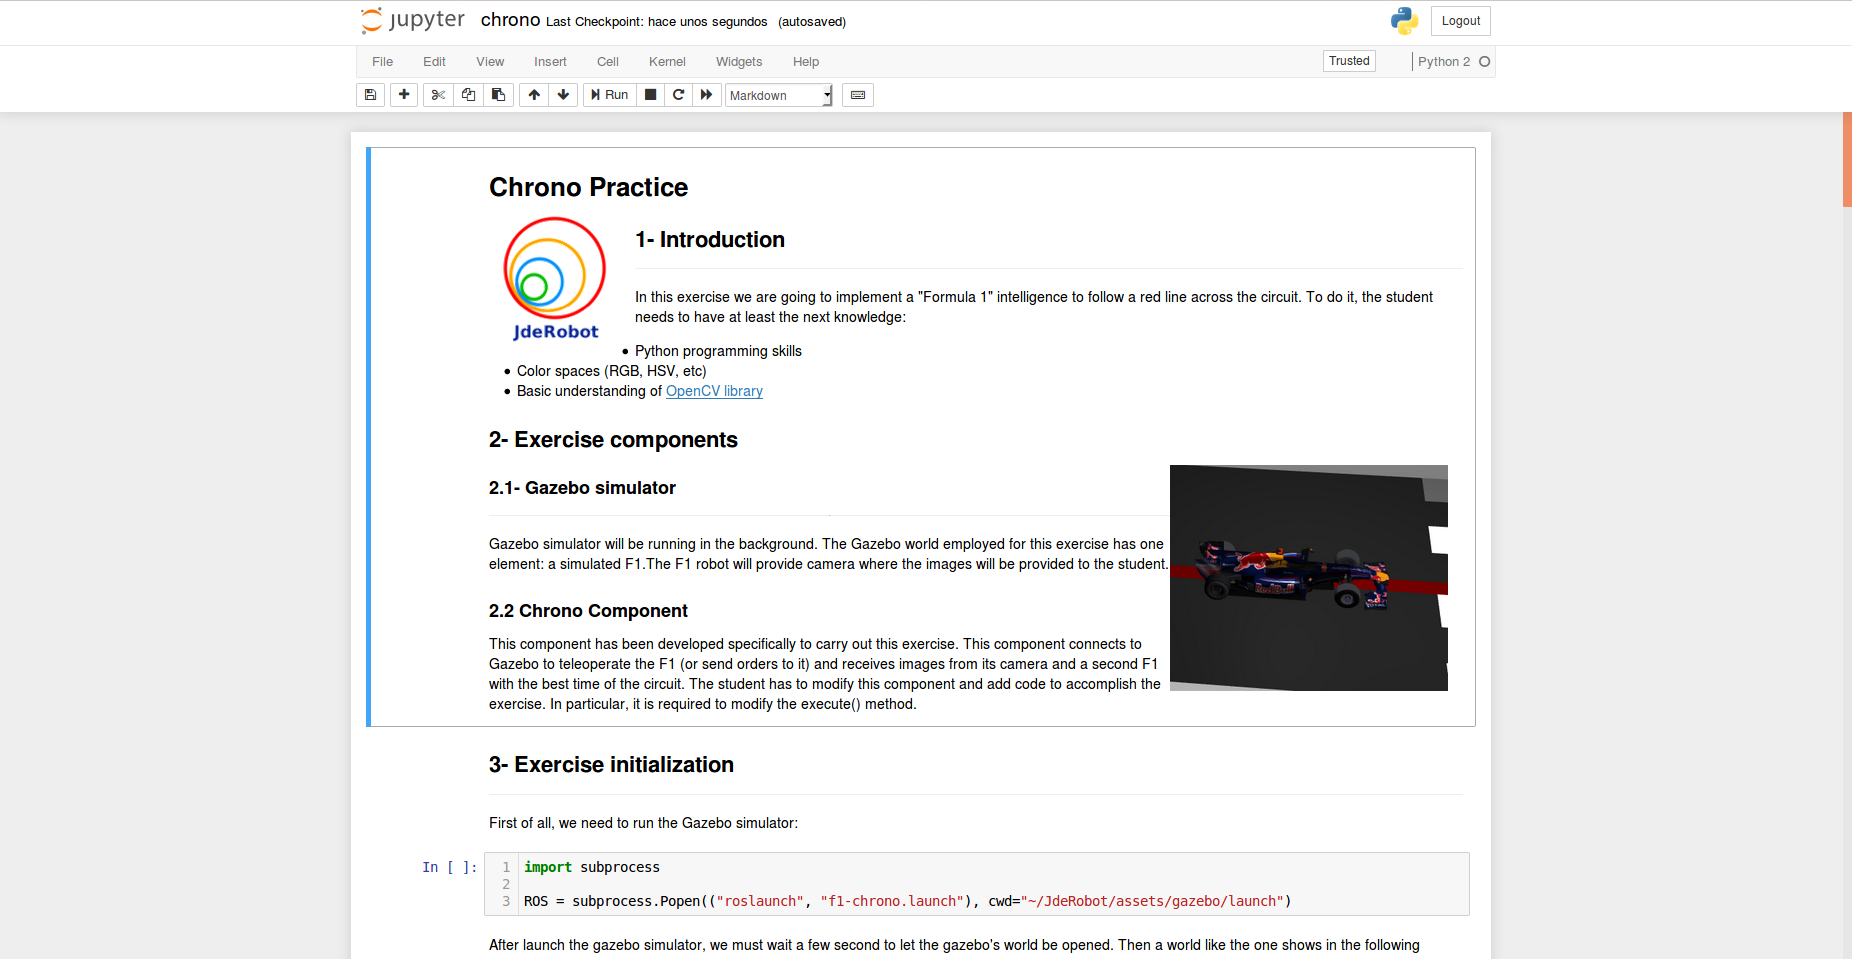
\includegraphics[width=0.98\textwidth]{figures/ipynb_chrono.png}
		\caption{Fichero Chrono.ipynb}
		\label{fig.fcipynb}
		\end{center}
\end{figure}

El alumno deberá ejecutar las celdas con código y seguir el guión mostrado. En primer lugar deberá ejecutar el fichero de configuración del mundo:

\begin{figure}[H]
  \begin{center}
    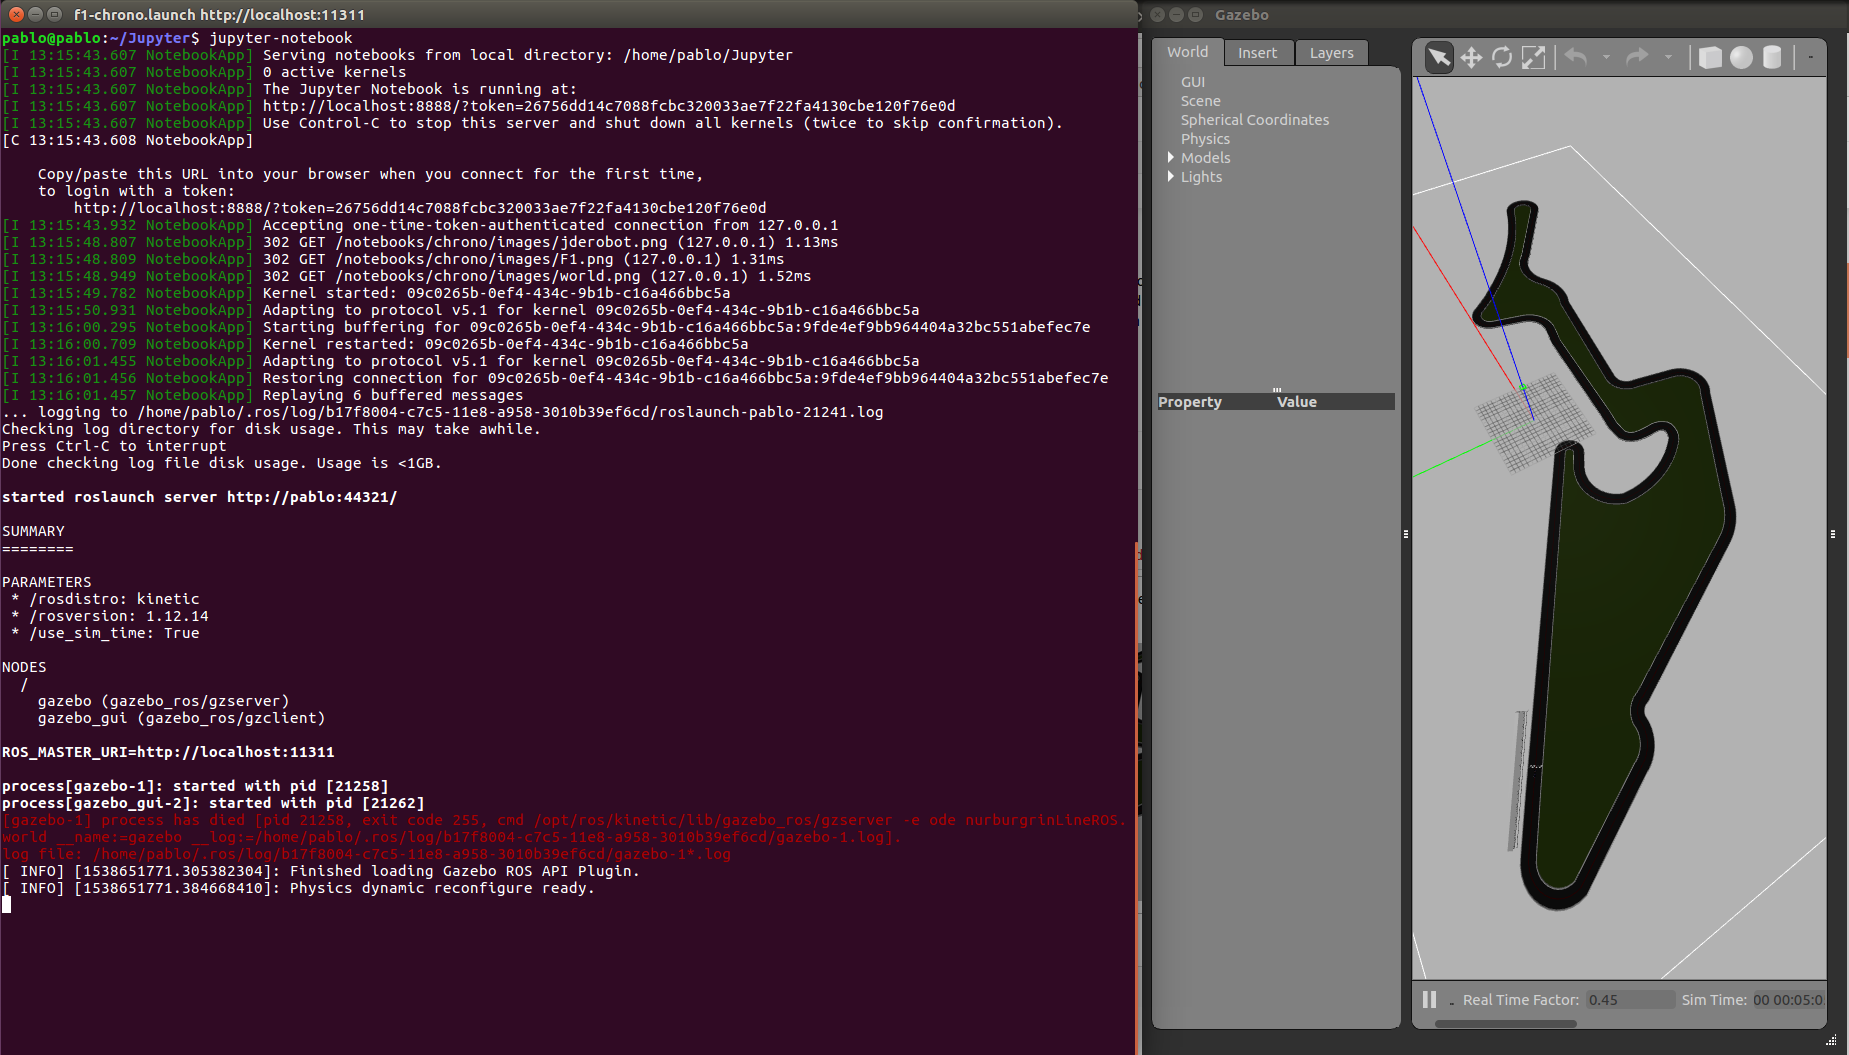
\includegraphics[width=0.98\textwidth]{figures/celda_mundo_chrono.png}
		\caption{Celda con la inicialización del mundo y los drivers}
		\label{fig.cmdc}
		\end{center}
\end{figure}

Cuando se haya abierto el simulador,es necesario importar el módulo del paquete ``MyAlgorithm.py'' y ``Chrono.py'' para tener la funcionalidad proveída en el nodo académico. Para ello, se ejecutará la siguiente celda con el nodo académico de la práctica:

\begin{figure}[H]
    \centering
	\begin{minipage}[h]{.48\linewidth}
    \centering
    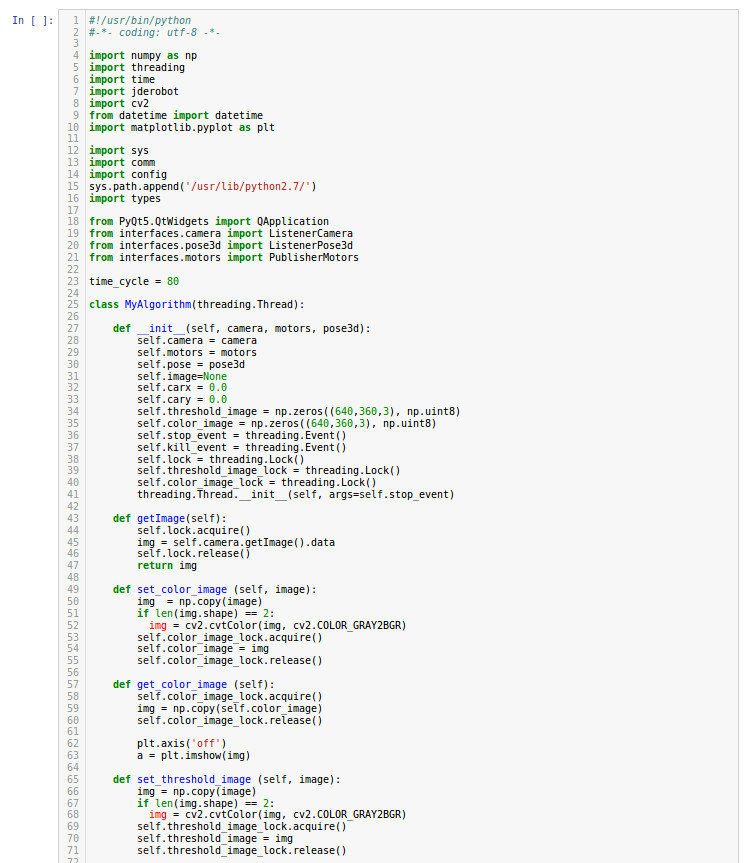
\includegraphics[width=0.98\textwidth]{figures/celda_nodo_chrono1.png}
	 \end{minipage}
    \begin{minipage}[h]{.48\linewidth}
    \centering
    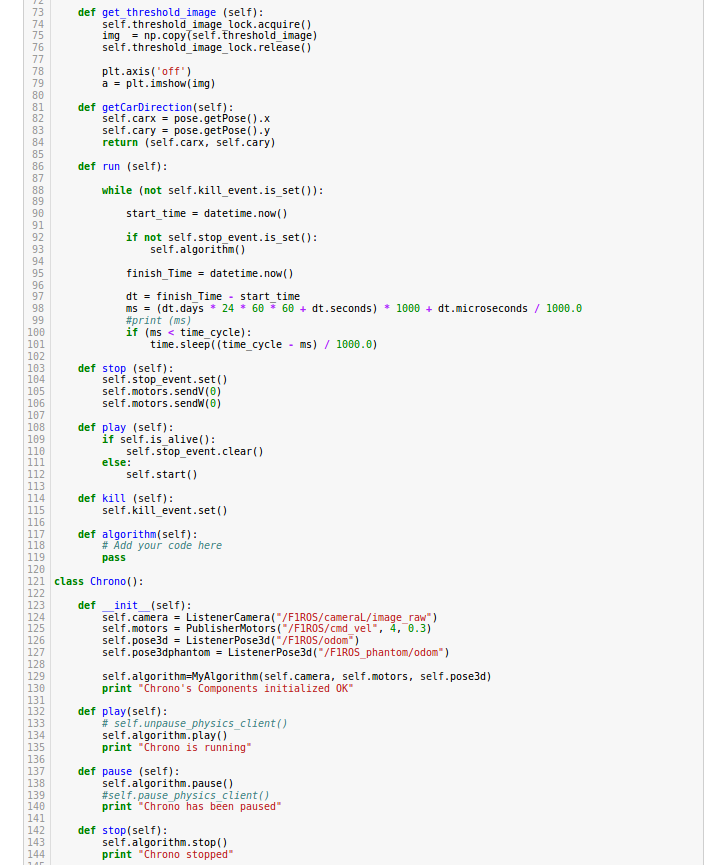
\includegraphics[width=0.98\linewidth]{figures/celda_nodo_chrono2.png}
	\end{minipage}
    \begin{minipage}[h]{.48\linewidth}
    \centering
    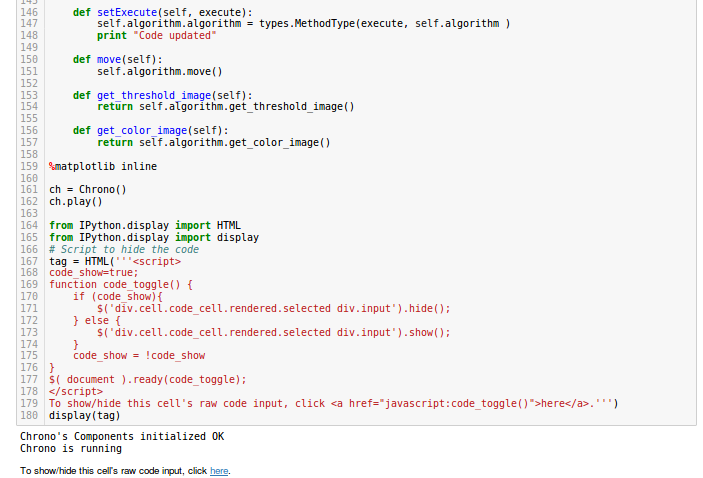
\includegraphics[width=0.98\linewidth]{figures/celda_nodo_chrono3.png}
	\end{minipage}
    \caption{Celda para importar el nodo académico}
		\label{fig.cnach}
\end{figure}


Cuando la ejecución imprima el mensaje ``OK''. El alumno puede comenzar a programar su código en la celda especificada para ello.

\begin{figure}[H]
  \begin{center}
    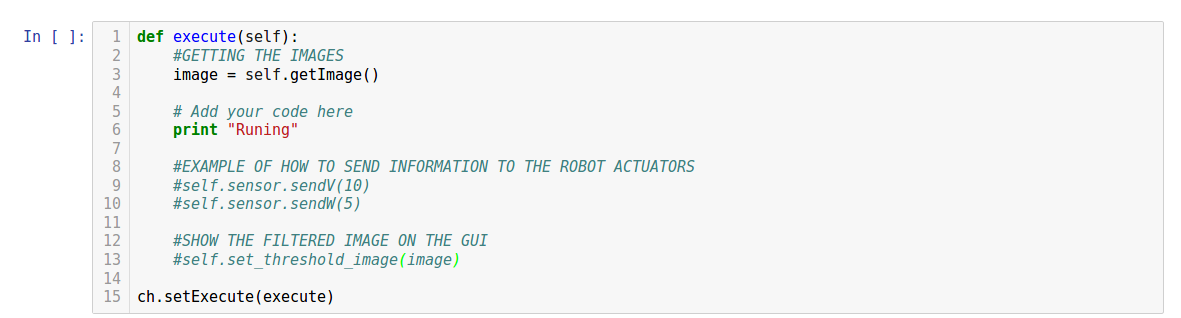
\includegraphics[width=0.98\textwidth]{figures/celda_solucion_chrono.png}
		\caption{Celda con el algoritmo del alumno}
		\label{fig.ccach}
		\end{center}
\end{figure}

Para comprobar el código desarrollado, basta con ejecutar la celda donde ha programado el algoritmo. Si quiere parar la ejecución, es suficiente con pulsar el botón con el icono de ``Stop'' del cuadernillo.

\begin{figure}[H]
    \centering
	\begin{minipage}[h]{.48\linewidth}
    \centering
    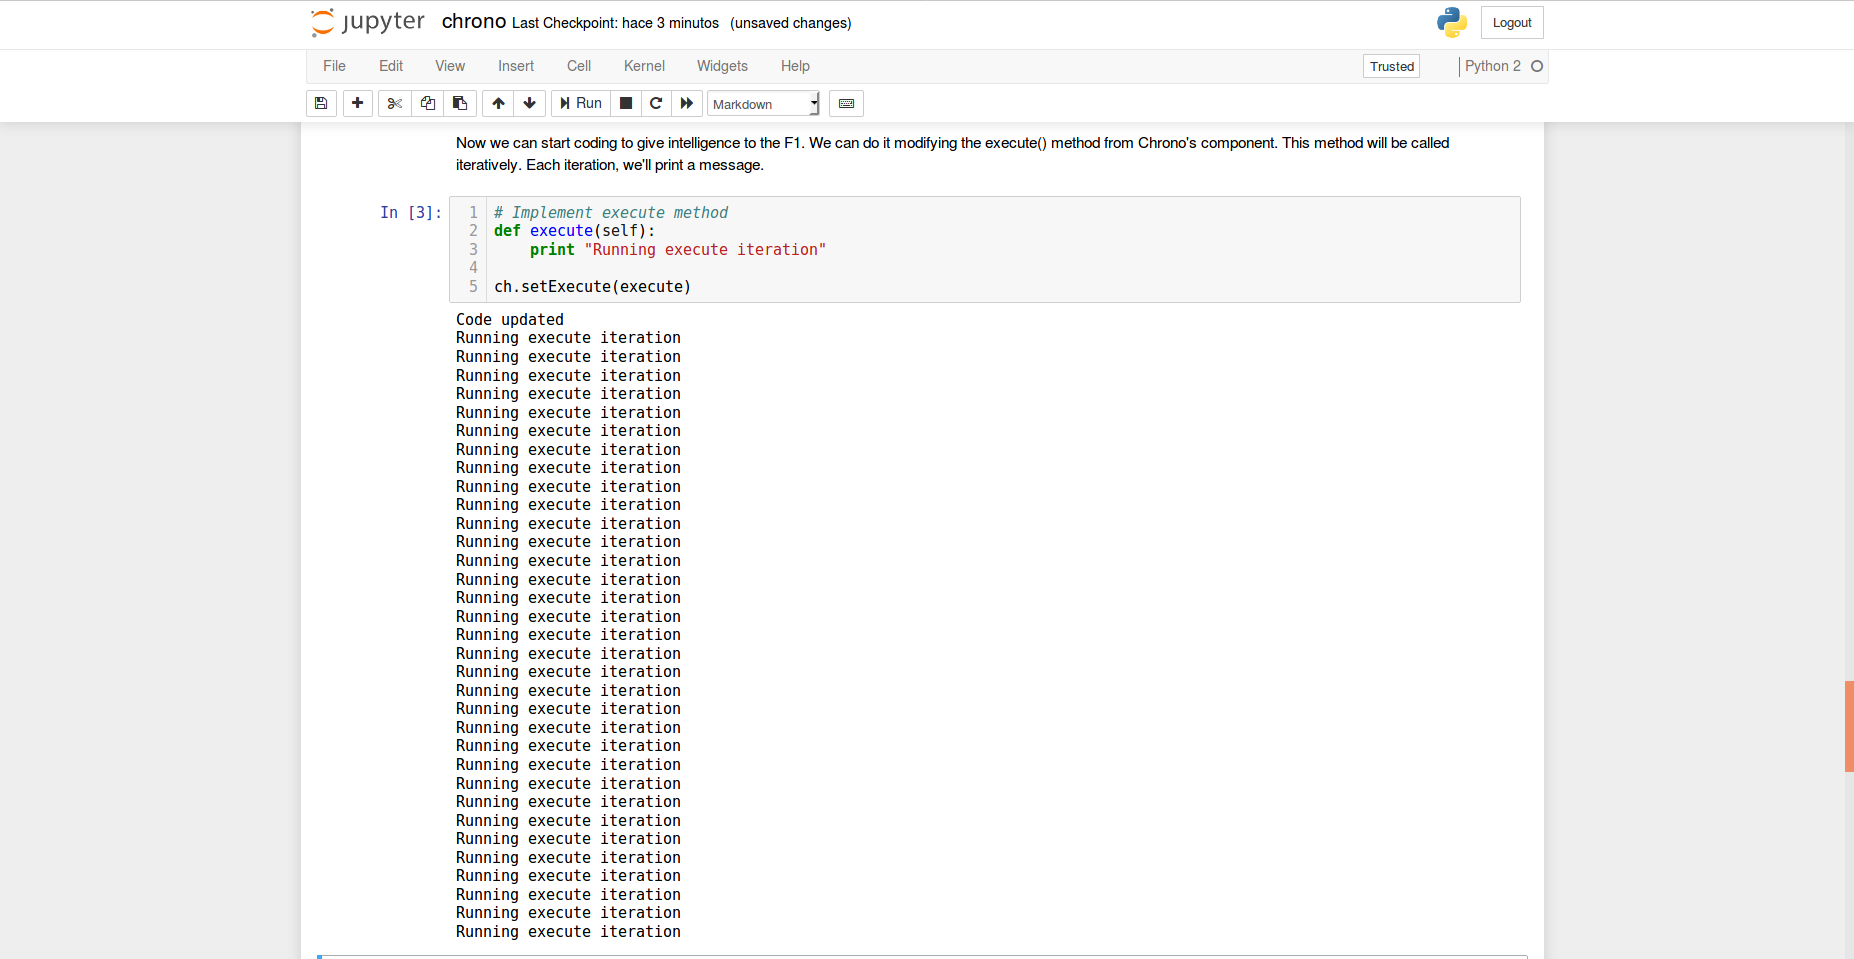
\includegraphics[width=0.98\textwidth]{figures/ejecucion_chrono_jupyter.png}
		\caption{Ejecución de la celda del algoritmo}
		\label{fig.ecj}
	 \end{minipage}
    \begin{minipage}[h]{.48\linewidth}
    \centering
    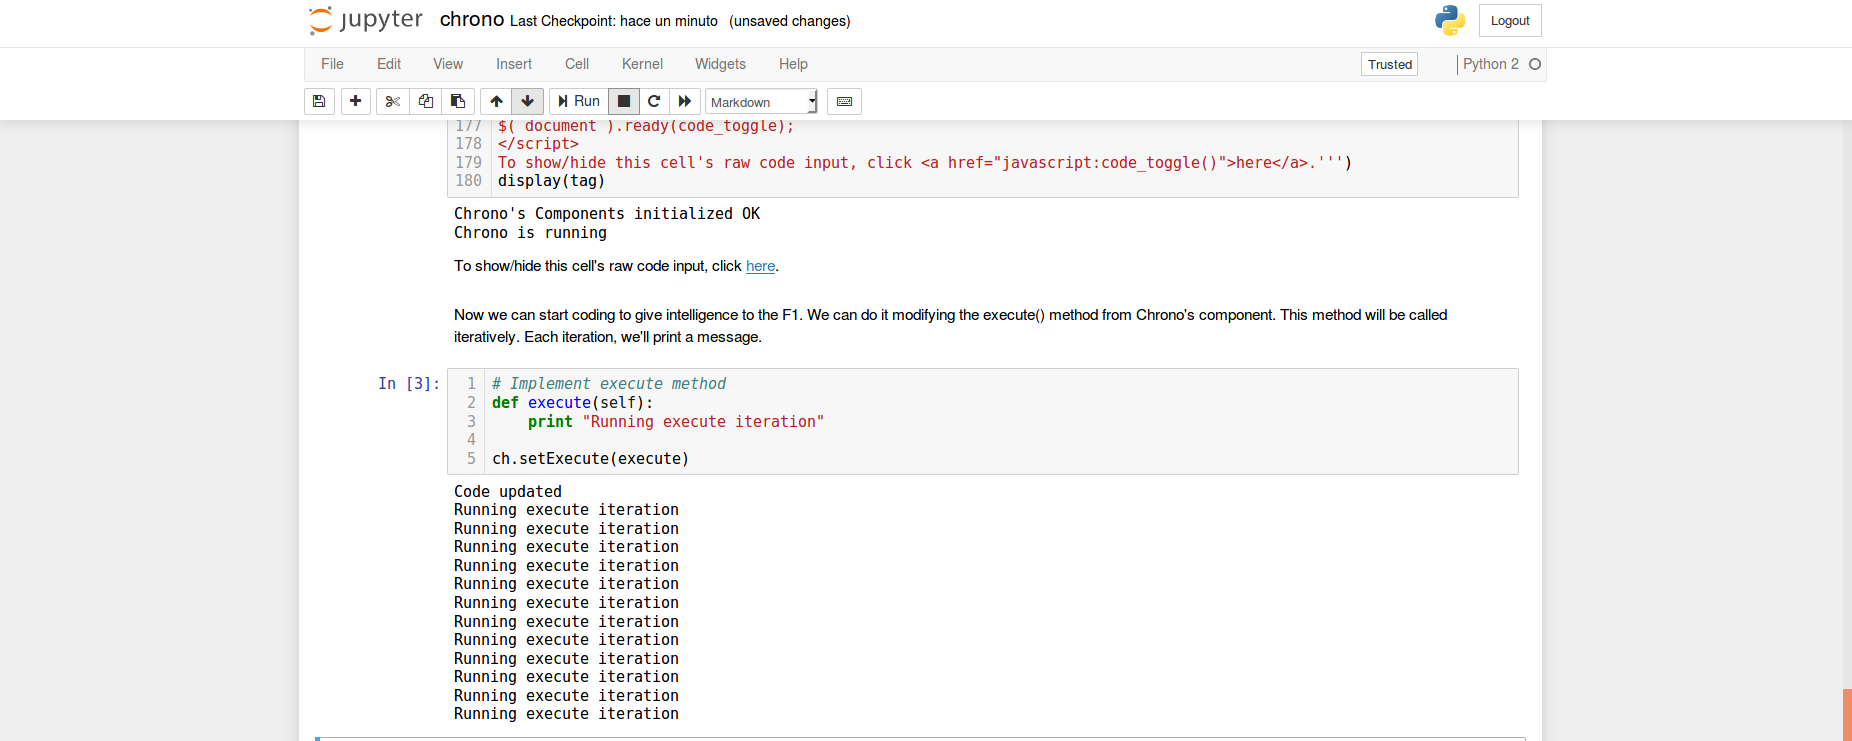
\includegraphics[width=0.98\linewidth]{figures/stop_chrono_jupyter.png}
		\captionof{figure}{Pausa de la ejecución del algoritmo}
		\label{fig:scj}
	\end{minipage}
\end{figure}

Puedes ver un vídeo de la ejecución de Jupyter con esta práctica.\footnote{\url{https://www.youtube.com/watch?v=vTAekepTRkQ}}
\lhead[]{CAP\'ITULO \thechapter. FOLLOW ROAD}
\chapter{Ejercicio de seguimiento automático de carreteras con drones}\label{cap.followroad}
Una vez descrita la práctica anterior, se va a proceder a la descripción de la segunda práctica desarrollada para el elenco de prácticas de robótica de \textit{JdeRobot}. Esta práctica se llama \textit{Follow Road} y se va a explicar todo lo relacionado con su infraestructura, el nodo académico, la solución desarrollada y su experimentación.

\section{Enunciado}\label{sec.enunciado}
El objetivo de esta práctica, enfocado al estudiante, es el desarrollo de un algoritmo que dote de la inteligencia necesaria a un dron par que sea capaz de seguir una carretera. En este caso, se deben controlar la altitud, la velocidad y el giro del dron para poder realizar un correcto seguimiento de la carretera, por parte del dron. Esto supone un desafío para el alumno que deberá tener un control absoluto del robot en todo momento.

Para desarrollar la solución de esta práctica, el alumno debe enfrentarse a diversos problemas relacionados con la robótica. El primero de ellos es la visión, el alumno deberá realizar un procesado de imagen para filtrar los componentes que le interesen, en este caso, deberá filtrar la carretera. El segundo problema a abordar, es el control de movimiento del dron, en este caso, debe ser muy preciso porque se manejan alturas, además de giros y velocidades. El último problema vienen derivado de los dos anteriores y supone realizar un movimiento controlado y dinámico del dron, para ello el alumno debe procesar las imágenes y realizar un movimiento controlado del dron en función de la imagen procesada.

El desafío de esta práctica reside en la dificultad de mantener el dron estable en todo momento y adecuar sus movimientos al procesado de imagen que se realice. Esto supone la afrontación de los problemas anteriores de manera conjunta. Además, es necesario el desarrollo de un algoritmo robusto para evitar que el dron se estrelle o tenga un comportamiento anormal en casos extremos o en situaciones no previstas.

\section{Infraestructura}
En esta sección se abordarán los distintos elementos involucrados en la práctica (Figura \ref{fig.inf_fr}).

%\begin{figure}[H]
%  \begin{center}
%    \includegraphics[width=0.99\linewidth, height=5.5cm]{figures/prueba.png}
%		\caption{Infraestructura de Chrono}
%		\label{fig.inf_chrono}
%		\end{center}
%\end{figure}

\subsection{Arquitectura}
La arquitectura de esta práctica es distinta a las existentes hasta ahora. Esto se debe a la utilización de paquetes ROS en el dron. Para el funcionamiento del dron con ROS, es necesario un soporte en \textit{C++} llamado \textit{MAVLink}. \textit{MAVLink} es un protocolo de comunicación para vehículos autómatas. Este protocolo proporciona los mensajes para comunicarse con el dron. Apoyado en \textit{MAVLink}, se encuentra \textit{MavROS}. Se trata de un nodo de \textit{ROS} que realiza un conversión entre los \textit{topics} que se utilizan en \textit{ROS} para comunicarse con los robots y los mensajes de \textit{MAVLink} permitiendo, de esta manera, la comunicación de los vehículos autónomos con \textit{ROS}.Además, proporciona los \textit{plugins} y \textit{topics} finales del dron. Por encima de \textit{MavROS}, se han desarrollado unos drivers específicos para permitir la comunicación de la infraestructura \textit{JdeRobot} con \textit{ROS}, de esta manera, la plataforma \textit{JdeRobot} es integrable con \textit{ROS Kinetic}.
En cuanto al control de robot o vehículo autónomo, se ha utilizado el software libre \textit{Px4}. Se trata de un sistema de pilotaje automático de drones especialmente orientado a pilotaje fuera de la línea de visión del usuario. Este \textit{sofware} aporta la infraestructura básica del dron.
La infraestructura completa de esta práctica puede verse en la figura \ref{fig.arquitectura_fr}.

%\begin{figure}[H]
%  \begin{center}
%    \includegraphics[width=0.99\linewidth, height=5.5cm]{figures/prueba.png}
%		\caption{Arquitectura de Follow Road}
%		\label{fig.arquitectura_fr}
%		\end{center}
%\end{figure}

\subsubsection{Modelo dron ``Iris''}
Este modelo de dron ha sido escogido para la realización de esta práctica. Consta de un cuerpo principal, en el que va instalado el \textit{hardware}, cuatro rotores, una antena y dos cámaras. La inteligencia del dron viene dada por el sistema de pilotaje automático \textit{Px4}.

\begin{figure}[H]
	\begin{center}
	    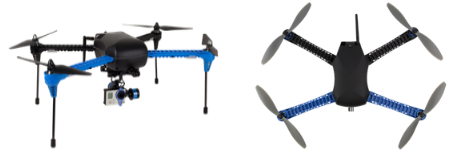
\includegraphics[width=0.98\textwidth]{figures/iris.png}
		\caption{Ilustraciones del dron ``Iris''}
		\label{fig.iris}
	\end{center}
\end{figure}

\subsubsection{Px4}
El piloto automático \textit{PX4}\footnote{\url{https://px4.io/}} es un sistema de piloto automático de código abierto orientado a aeronaves autónomas de bajo coste. Tanto el \textit{hardware} como el \textit{software} es \textit{open-source} y accesible gratuitamente bajo una licencia \textit{BSD}. Esta plataforma, derivó del proyecto \textit{PIXHWAK}\footnote{\url{http://pixhawk.org/}} que se centró, específicamente, en control de vuelo basado en visión. El \textit{software} incluido bajo \textit{Px4} incluye:
\begin{itemize}
    \item QGroundControl\footnote{\url{http://qgroundcontrol.com/}} y MAVLink para las comunicaciones con el dron.
    \item Mapas aéreos en 2D y 3D con soporte de Google Earth\footnote{\url{https://www.google.com/earth/}}.
    \item Puntos de control \textit{Drag-and-Drop}.
\end{itemize}

Esta infraestructura ha sido escogida por su compatibilidad de comunicaciones mediante el protocolo \textit{MAVLink}. Además, este sistema de autopilotaje tiene distintas características que lo convierten en la opción escogida para soporte de \textit{hardware} y \textit{software} de \textit{JdeRobot}:
\begin{itemize}
    \item Arquitectura modular y extensible.
    \item Código base simple para todos los vehículos.
    \item Desarrollado para conducción autónoma.
    \item Gran conjunto de periféricos compatibles.
    \item Modos de vuelo flexibles y potentes.
    \item Dispone de herramientas complementarias de desarrollo.
    \item Probado en modelos reales.
    \item Código \textit{open-source}.
\end{itemize}

Para esta práctica se ha utilizado la comunicación con el dron bajo los mensajes \textit{MAVLink}. De esta manera, \textit{Px4}, realiza la conversión de mensajes \textit{MAVLink} a comandos para el dron y viceversa.

\subsubsection{MAVLink}
El \textit{software} libre \textit{MAVLink}\footnote{\url{https://mavlink.io/en/}} (Micro Air Vehicle Link), es un protocolo de mensajes de comunicación en vehículos autónomos. Se ha diseñado como una librería de cálculo de referencia de encabezado simple. Fue lanzado a principios del año 2009 por Lorenz Meier bajo una licencia \textit{LGPL}\footnote{\url{https://en.wikipedia.org/wiki/GNU_Lesser_General_Public_License}}.

Los mensajes están definidos con ficheros \textit{XML}. Cada fichero \textit{XML} define un conjunto de mensajes admitidos por un sistema \textit{MAVLink} particular o dialecto.

\subsubsection{MavROS}
El nodo de \textit{ROS}, \textit{MavROS}\footnote{\url{http://wiki.ros.org/mavros}}\footnote{\url{http://ardupilot.org/dev/docs/ros.html}}, es un paquete que proporciona un controlador de comunicación para varios pilotos automáticos con el protocolo de comunicación \textit{MAVLink} y un puente \textit{UDP MAVLink} para estaciones de control terrestre.

\textit{MavROS} esta formado por cuatro componentes:
\begin{itemize}
    \item Nodos \textit{MavROS}. Estos nodos están formados por \textit{topics} de suscripción, \textit{topics} de publicación y parámetros de configuración.
    \item Puente \textit{GCS}. Es la conexión de \textit{MavROS} con el protocolo de mensajes \textit{MAVLink}.
    \item Lanzador de eventos. Comprueba el estado de los eventos producidos por los \textit{topics}.
    \item \textit{Plugins}. \textit{MavROS} proporciona un gran número de \textit{topics} a los que poder suscribirte para recibir información del estado del dron o para publicar comandos de control del dron. A este conjunto de \textit{plugins} se accede gracias a los \textit{topics}. Cada \textit{plugins} contiene distintos \textit{topics} o tipos de mensajes distintos con los que enviar o recibir información del \textit{plugin}. Una vez recibida esta información, el \textit{plugin} realiza una transformación de mensajes \textit{MAVLink} a \textit{topics} de \textit{ROS} y viceversa.  Los \textit{topics} ofrecidos por los \textit{plugins} de \textit{MavROS} son más de cien pero, para el control del dron en \textit{JdeRobot}, se han utilizado los siguientes:
        \item /mavros/cmd/arming: para armar el dron.
        \item /mavros/global\_position/global: para conocer la posición gps del dron y realizar el despegue.
        \item /mavros/cmd/takeoff: para despegar el dron.
        \item /mavros/cmd/land: para aterrizar el dron.
        \item /mavros/set/mode: para cambiar el dron entre sus distintos modos.
            \item Auto\_RTL: Modo automático. Se utiliza para despegar y aterrizar.
            \item Offboard: Modo manual. Se utiliza para controlar el dron.
        \item /mavros/setpoint\_raw/local: para controlar el movimiento del dron. Permite enviar información de posición, altura, velocidad, aceleración y giro. 
        \item /mavros/local\_position/odom: para recibir la odometría del dron.
        \item /iris\_fpv\_cam/cam\_XXXXX/image\_raw: aunque no se trata de un \textit{topic} proporcionado por \textit{MavROS}, utiliza \textit{ROS} para recibir información de las cámaras, por lo que es integrable con \textit{MavROS}.
\end{itemize}

\subsubsection{Drivers}
Para realizar las conexiones a los \textit{topics} ofrecidos por \textit{MavROS}, se han desarrollado unos drivers, específicos para la infraestructura de \textit{JdeRobot}. Para ello se han desarrollado un total de seis ficheros con código en \textit{Python} que dotan de la infraestructura necesaria, al nodo académico, para comunicarse con el dron.

\begin{itemize}
    \item En el fichero \textit{\_\_init\_\_.py}, se establecen las cabeceras de las funciones principales de interconexión y las conexiones de los \textit{topics}.
    \item En el fichero \textit{camera.py}, se han desarrollado las funciones necesarias para recoger las imágenes captadas por las cámaras integradas en el dron.
    \item En el fichero \textit{cmdvel.py}, se incorporan las funciones necesarias para enviar los comandos de velocidad al plugin de \textit{MavROS}.
    \item En el fichero \textit{extra.py}, se han desarrollado las funciones para controlar el despegue y aterrizaje del dron.
    \item En el fichero \textit{pose3d.py}, están las funciones para recoger la información sobre la odometría del dron.
    \item En el fichero \textit{threadPublisher.py}, está la función de creación de la hebra para las comunicaciones de las hebras de publicación de \textit{topics}.
\end{itemize}


\subsubsection{Sensores y actuadores}
Una vez descritos los componentes de comunicación con el dron, se va a explicar los componentes que forman el modelo del dron. Estos componentes dotan al dron de la estructura y movilidad necesaria para su funcionamiento.

\paragraph{Cámara}
La cámara proporciona al dron visión del escenario en el que se encuentra. Es necesaria para dotar al dron de una interfaz sobre la que basar su inteligencia. En esta práctica son necesarias dos cámaras, una frontal y otra ventral para tener un visión del entorno tanto en la parte delantera del dron, para evitar obstáculos, como inferior para poder visualizar correctamente la carretera.

El \textit{plugin} de la cámara es proporcionado por \textit{ROS}. Este \textit{plugin} proporciona el código necesario para conectar una cámara mediante USB con una velocidad de refresco de 30 imágenes por segundo  con una longitud focal de 277 milímetros. Con estas características, el dron puede recoger imágenes a una velocidad lo suficientemente rápida y a una distancia apropiada, para procesar las imágenes y conseguir evitar los obstáculos con suficiente antelación.

Las imágenes captadas por la cámara son recogidas por el nodo académico gracias a su interfaz gráfica y mediante un API simple. De esta manera se pueden visualizar las imágenes de las cámaras en la interfaz gráfica del nodo académico, así como su procesado.

\paragraph{Sensor Odométrico}
Con este sensor, el dron es capaz de conocer su posición. Este sistema se implementa gracias al GPS que incorpora el dron y le permite conocer su latitud y longitud en el escenario en el que se encuentre. \textit{MavROS} incorpora \textit{topics} para conocer esta posición. El \textit{topic} utilizado para estimar esta posición ofrece la posición del dron en coordenadas relativas al lugar de despegue del dron. Esta funcionalidad viene soportada en el \textit{plugin setpoint\_position}.

\paragraph{Rotores}
El dron está formado por cuatro rotores que permite su movimiento. Para el control de estos rotores, se incorpora un \textit{plugin} de control de rotor por cada uno de los rotores del dron. Este \textit{plugin} es proporcionado por \textit{Px4} y es de \textit{ROS}. Sin embargo, el \textit{plugin} que se utiliza para mover el dron es proporcionado por \textit{MavROS} bajo el nombre \textit{setpoint\_raw} al que se accede con el \textit{topic /mavros/setpoint\_raw/local}. 

\paragraph{Escenario de Gazebo}
Para esta práctica se ha actualizado el escenario inicial del que disponía la práctica y se han arreglado problemas que presentaba relacionados con la visualización del suelo, un nuevo modelo de casa y la incorporación del modelo del dron nuevo. El aspecto del escenario puede verse en la figura \ref{fig.mundo_fr}.

\begin{figure}[H]
  \begin{center}
    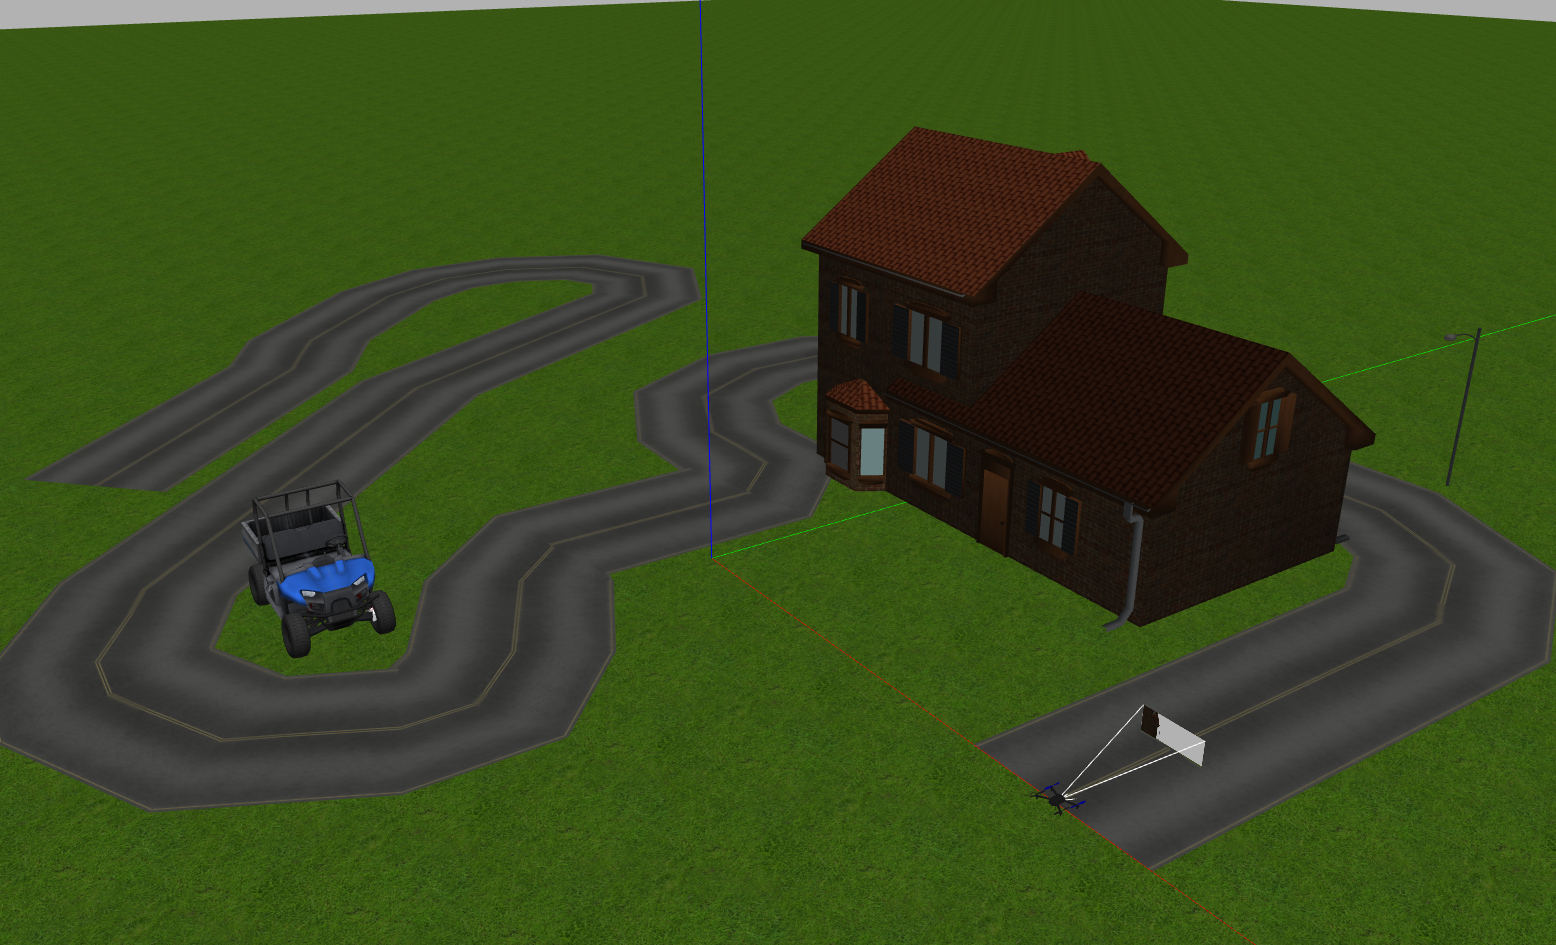
\includegraphics[width=0.9\linewidth]{figures/mundo_fr.png}
		\caption{Escenario de Follow Road}
		\label{fig.mundo_fr}
		\end{center}
\end{figure}

\paragraph{Ficheros de configuración} \label{sec.launch_fr}
Para la incorporación del modelo del circuito y del robot, es necesario la creación de un modelo de configuración que importe en \textit{Gazebo} los elementos de los que consta el escenario y su localización. Este fichero tiene la extensión \textit{.world} y \textit{Gazebo} es capaz de leerlo y mostrar el escenario al iniciarse.
El código del fichero es el siguiente:

\lstset{language=XML, breaklines=true, basicstyle=\footnotesize}
\begin{lstlisting}[frame=single]
<?xml version="1.0" ?>
<sdf version="1.5">
  <world name="default">
    <scene>
      <grid>false</grid>
    </scene>
    <!-- A global light source -->
    <include>
      <uri>model://sun</uri>
    </include>
    <include>
      <uri>model://grass_plane</uri>
    </include>

    <include>
      <uri>model://house_4</uri>
      <pose>1 6.43 0 0 0 0</pose>
    </include>
    <include>
      <uri>model://polaris_ranger_ev</uri>
      <pose>-1.48 -6 0.1 0 0 0</pose>
      <static>true</static>
    </include>
    <include>
      <uri>model://lamp_post</uri>
      <pose>5 13 0 0 0 0</pose>
    </include>
    <include>
      <uri>model://lamp_post</uri>
      <pose>-4 13 0 0 0 0</pose>
    </include>
    <include>
      <uri>model://iris_fpv_cam</uri>
      <pose>8 0 0.3 0 0 1.57</pose>
    </include>
    <road name="my_road">
      <width>3</width>

      <point>8 0 0.01</point>
      <point>8 3 0.01</point>
      <point>8 8 0.01</point>
      <point>7 10 0.01</point>
      <point>5 11 0.01</point>
      <point>-5 11 0.01</point>
      <point>-7 10 0.01</point>
      <point>-8 8 0.01</point>
      <point>-8 6 0.01</point>
      <point>-7 4 0.01</point>
      <point>-5 3 0.01</point>
      <point>-3 3 0.01</point>
      <point>-2 2 0.01</point>
      <point>-2 -2 0.01</point>
      <point>-1 -3 0.01</point>

      <point>1 -4 0.01</point>
      <point>2 -5 0.01</point>

      <point>2 -6 0.01</point>
      <point>1 -8 0.01</point>
      <point>-1 -9 0.01</point>
      <point>-2 -9 0.01</point>
      <point>-4 -8 0.01</point>

      <point>-11 -1 0.01</point>
      <point>-14 5 0.01</point>

      <point>-15 7 0.01</point>
      <point>-17 8 0.01</point>
      <point>-19 7 0.01</point>

      <point>-20 5 0.01</point>
      <point>-20 3 0.01</point>
      <point>-19 1 0.01</point>
      <point>-17 -1 0.01</point>

      <point>-16 -2 0.01</point>
      <point>-14 -3 0.01</point>
      <point>-9 -8 0.01</point>
    </road>
  </world>
</sdf>
\end{lstlisting}

Además de este fichero de configuración, es necesario un fichero complementario que importe los \textit{plugins y drivers} de ROS-Kinetic. Este tipo de fichero tienen la extensión \textit{.launch}. En este fichero se pasan a \textit{Gazebo} argumentos como el nombre del fichero de configuración con el escenario, establecer el tiempo que se va a utilizar en el escenario, la posible implementación de un GUI y otras opciones de depuración.
El fichero es el siguiente:

\lstset{language=XML, breaklines=true, basicstyle=\footnotesize}
\begin{lstlisting}[frame=single]
<?xml version="1.0" encoding="UTF-8"?>
<launch>
  <!-- We resume the logic in empty_world.launch, changing only the name of the world to be launched -->
  <include file="$(find gazebo_ros)/launch/empty_world.launch">
    <arg name="world_name" value="road_drone_textures_ROS.world"/> <!-- Note: the world_name is with respect to GAZEBO_RESOURCE_PATH environmental variable -->
    <arg name="paused" value="false"/>
    <arg name="use_sim_time" value="true"/>
    <arg name="gui" value="true"/>
    <arg name="headless" value="false"/>
    <arg name="debug" value="false"/>
    <arg name="verbose" default="true"/>
  </include>

  <arg name="fcu_url" default="udp://:14540@127.0.0.1:14540" />
	<arg name="gcs_url" default="" />
	<arg name="tgt_system" default="1" />
	<arg name="tgt_component" default="1" />
	<arg name="log_output" default="screen" />
	<arg name="fcu_protocol" default="v2.0" />
	<arg name="respawn_mavros" default="false" />

	<include file="$(find mavros)/launch/node.launch">
		<arg name="pluginlists_yaml" value="$(find mavros)/launch/px4_pluginlists.yaml" />
		<arg name="config_yaml" value="$(find mavros)/launch/px4_config.yaml" />

		<arg name="fcu_url" value="$(arg fcu_url)" />
		<arg name="gcs_url" value="$(arg gcs_url)" />
		<arg name="tgt_system" value="$(arg tgt_system)" />
		<arg name="tgt_component" value="$(arg tgt_component)" />
		<arg name="log_output" value="$(arg log_output)" />
		<arg name="fcu_protocol" value="$(arg fcu_protocol)" />
		<arg name="respawn_mavros" default="$(arg respawn_mavros)" />
	</include>

  <node pkg="mavros" type="px4.sh"  name="px4" output="screen"/>
</launch>
\end{lstlisting}

\subsection{Arquitectura software}
Esta práctica tiene tes hilos de ejecución para aliviar la carga computacional de la práctica De esta manera se aumenta la velocidad  la que puede trabajar el simulador \textit{Gazebo}.

\begin{itemize}
	\item Hilo de sensores: este hilo se encarga de la actualización de los datos de los sensores del robot. Este hilo se comunica con \textit{Gazebo} para recoger datos de la odometría y la cámara y entregárselos al nodo académico.
	\item Hilo de la interfaz gráfica del usuario (GUI): este hilo se encarga del refresco del GUI de la práctica. En esta práctica tiene una carga computacional elevada dado se encarga de refrescar las imágenes obtenidas por la cámaras, el procesamiento visual sobre esa imagen que ha realizado el alumno, un mapa del circuito con la posición actualizada del robot y del robot fantasma a vencer, y una lectura controlada de tiempos para sincronizar ambos coches.
	\item Hilo de actuadores: este hilo se encarga de enviar la información del nodo académico al dron. Se conecta con \textit{Gazebo} para enviar las órdenes de movimiento.
\end{itemize}

\subsubsection{Interfaz gráfica}
La interfaz gráfica del usuario (GUI), se utiliza para representar información relacionada con los sensores del robot. Esta información es muy útil para la depuración del algoritmo del estudiante ya que permite la visualización de las publicaciones que realiza el algoritmo al robot.

Esta GUI (Figura \ref{fig.guifr}) está formada por tres conjuntos \textit{widgets}, uno para el visionado del de las imágenes, otro para su control y otro para el teleoperador.

\begin{figure}[H]
  \begin{center}
    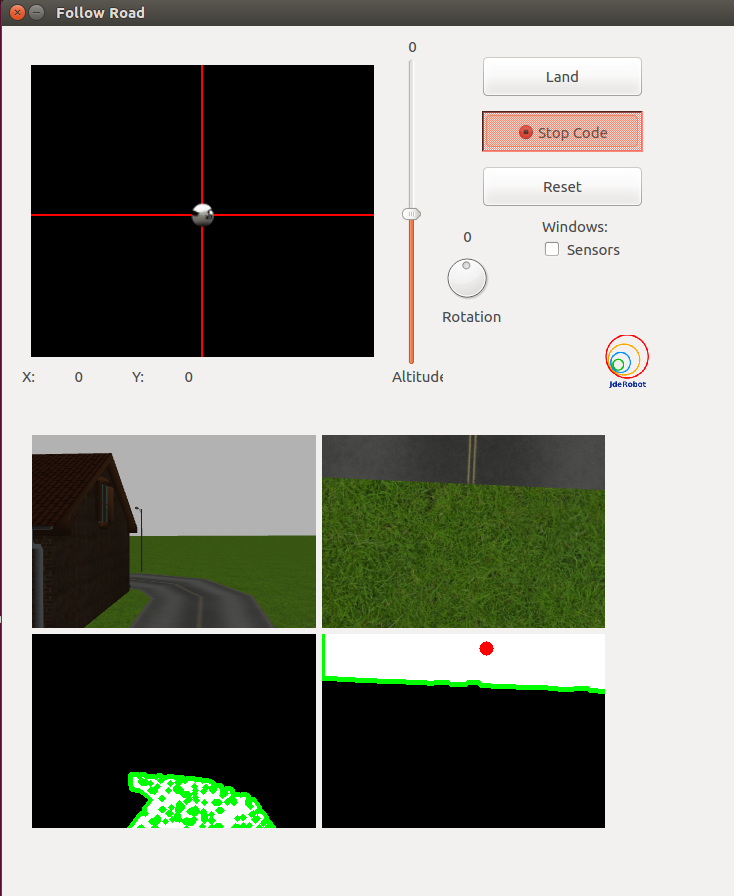
\includegraphics[width=7cm,height=10cm,\textwidth]{figures/GUI_fr.png}
		\caption{Interfaz Gráfica Folow Road}
		\label{fig.guifr}
		\end{center}
\end{figure}

El \textit{widget} del teleoperador se utiliza para controlar el dron una vez ha despegado. De esta manera se puede comprobar que las conexiones del dron están correctamente realizadas.

El conjunto \textit{widgets} destinados al control del dron se dividen en tres subconjuntos:
\begin{itemize}
    \item Control de altitud y rotación.
    \item wirdgets de estabilización.
    \item Botón de despegue/aterrizaje, botón de ejecución y parada del algoritmo de solución y botón de reinicio del puntero del teleoperador.
\end{itemize}
Con estos \textit{widgets} se puede controlar el dron de manera manual o mediante la programación de la inteligencia del dron en el fichero de solución.

El \textit{widget} de visionado del dron incorpora cuatro pantallas. Las pantallas superiores reflejan las imágenes recogidas por las cámaras del dron y las pantallas inferiores muestran el procesado de las imágenes realizado en el algoritmo del solución del alumno. Este último \textit{widget} es muy útil para depurar el algoritmo del alumno ya que puede verse, fácilmente, el procesado que se ha realizado de la imagen.

\section{Nodo Académico}
Una vez explicado toda la infraestructura circundante al nodo académico de la práctica, se va a explicar la infraestructura del propio nodo. Esta formado por:

\begin{itemize}
    \item Fichero principal.
    \item Fichero de solución
    \item GUI. Directorio con todos los ficheros para el funcionamiento del GUI.
\end{itemize}

El fichero principal es el código que va a ejecutarse para lanzar el nodo académico de la práctica. En él se especifican las conexiones con los \textit{topics} que se van a establecer, así como la inizalización del GUI.

En el fichero de solución, hay un conjunto de funciones que aportan la funcionalidad de la práctica, como comenzar, parar, recoger imagen, así como las que desarrolle el alumno y el propio código con la solución de referencia.

\section{Solución de referencia}
Para esta práctica se han desarrollado dos soluciones de referencia. La primera solución se ha desarrollado para la práctica inicial que no contaba con soporte para \textit{ROS} y se realizaba con \textit{drivers ICE}. La segunda solución desarrollada es compatible con \textit{ROS}. Ambas soluciones han sido desarrolladas íntegramente.

\subsection{Procesamiento de imagen}
El procesamiento de las imágenes programado se ha realizado en función del contorno del filtrado. Para ello se comienza con la recogida de las imágenes captadas por la cámara:

\lstset{language=Python, breaklines=true, basicstyle=\footnotesize}
\begin{lstlisting}[frame=single]
input_imageV = self.drone.getImageVentral().data
input_imageF = self.drone.getImageFrontal().data
\end{lstlisting}

Con esta instrucción, es posible visualizar las imágenes en el GUI.

Tras obtener las imágenes frontal y ventral de la cámara, hay que transformarla a una imagen HSV\footnote{\url{https://es.wikipedia.org/wiki/Modelo_de_color_HSV}} para poder seleccionar el color de la carretera:

\lstset{language=Python, breaklines=true, basicstyle=\footnotesize}
\begin{lstlisting}[frame=single]
image_HSV_V = cv2.cvtColor(input_imageV, cv2.COLOR_RGB2HSV)
image_HSV_F = cv2.cvtColor(input_imageF, cv2.COLOR_RGB2HSV)
\end{lstlisting}

Tras obtener la imagen HSV, podemos seleccionar el rango de valores que componen color de la carretera como un array con la intensidad mínima y máxima del color.

\lstset{language=Python, breaklines=true, basicstyle=\footnotesize}
\begin{lstlisting}[frame=single]
value_min_HSV = np.array([20, 0, 0])
value_max_HSV = np.array([100, 130, 130])
\end{lstlisting}

Con esos valores realizamos un filtrado de la imagen para obtener la carretera, exclusivamente:

\lstset{language=Python, breaklines=true, basicstyle=\footnotesize}
\begin{lstlisting}[frame=single]
image_HSV_filtered_V = cv2.inRange(image_HSV_V, value_min_HSV, value_max_HSV)
image_HSV_filtered_F = cv2.inRange(image_HSV_F, value_min_HSV, value_max_HSV)
\end{lstlisting}

Para reducir el ruido que contiene la la imagen sobre los colores filtrados es necesario aplicar técnicas de reducción de ruido. Para ello hemos realizado una apertura y un cierre de la imagen:

\lstset{language=Python, breaklines=true, basicstyle=\footnotesize}
\begin{lstlisting}[frame=single]
opening_V = cv2.morphologyEx(image_HSV_filtered_V, cv2.MORPH_OPEN, np.ones((5,5),np.uint8))
closing_V = cv2.morphologyEx(opening_V, cv2.MORPH_CLOSE, np.ones((10,10),np.uint8))
\end{lstlisting}

Para el caso de la imagen frontal, hemos realizado una técnica de apertura, solamente, con lo que se obtendrá más ruido que con la combinación anterior:

\lstset{language=Python, breaklines=true, basicstyle=\footnotesize}
\begin{lstlisting}[frame=single]
opening_F = cv2.morphologyEx(image_HSV_filtered_F, cv2.MORPH_OPEN, np.ones((5,5),np.uint8))
\end{lstlisting}

Una vez tenemos el filtro, lo utilizamos como una máscara para realizar el filtrado de la imagen y obtiener la imagen filtrada en formato binario, con el rango de colores que pasan el filtro en blanco:

\lstset{language=Python, breaklines=true, basicstyle=\footnotesize}
\begin{lstlisting}[frame=single]
image_HSV_filtered_Mask_V = np.dstack((closing_V, closing_V, closing_V))
image_HSV_filtered_Mask_F = np.dstack((opening_F, opening_F, opening_F))
\end{lstlisting}

Una vez realizado el filtrado, es necesario convertir la imagen a escala de grises para poder dibujar el contorno de la sección filtrada:

\lstset{language=Python, breaklines=true, basicstyle=\footnotesize}
\begin{lstlisting}[frame=single]
imgray_V = cv2.cvtColor(image_HSV_filtered_Mask_V, cv2.COLOR_BGR2GRAY)
ret_V, thresh_V = cv2.threshold(imgray_V, 127, 255, 0)
_, contours_V, hierarchy_V = cv2.findContours(thresh_V, cv2.RETR_TREE, cv2.CHAIN_APPROX_SIMPLE)
cv2.drawContours(image_HSV_filtered_Mask_V, contours_V, -1, (0,255,0), 3)

imgray_F = cv2.cvtColor(image_HSV_filtered_Mask_F, cv2.COLOR_BGR2GRAY)
ret_F, thresh_F = cv2.threshold(imgray_F, 127, 255, 0)
_, contours_F, hierarchy_F = cv2.findContours(thresh_F, cv2.RETR_TREE, cv2.CHAIN_APPROX_SIMPLE)
cv2.drawContours(image_HSV_filtered_Mask_F, contours_F, -1, (0,255,0), 3)
\end{lstlisting}

Tras dibujar el contorno de la sección, es necesaria una comprobación del filtrado de la imagen para evitar errores en la ejecución. El siguiente algoritmo comprueba si se ha recogido alguna imagen, si hay alguna zona que ha pasado el filtro y se hay más de una sección filtrada (para el caso en que se detecten varias carreteras):

\lstset{language=Python, breaklines=true, basicstyle=\footnotesize}
\begin{lstlisting}[frame=single]
area = []
for pic, contour in enumerate(contours_V):
    area.append(cv2.contourArea(contour))

if len(area) > 1:
    if area[0] < area[1]:
        M = cv2.moments(contours_V[1])
    else:
        M = cv2.moments(contours_V[0])

else:
    try:
        M = cv2.moments(contours_V[0])
    except IndexError:
        self.drone.sendCMDVel(0,0.3,0,0)
        M = cv2.moments(0)
\end{lstlisting}

Si la comprobación es exitosa, se extraen las coordenadas del centro de la sección filtrada:

\lstset{language=Python, breaklines=true, basicstyle=\footnotesize}
\begin{lstlisting}[frame=single]
if int(M['m00']) != 0:
    cx = int(M['m10']/M['m00'])
    cy = int(M['m01']/M['m00'])
\end{lstlisting}

Se dibuja un punto rojo para saber el centro de la sección filtrada, punto el cual seguirá el dron:

\lstset{language=Python, breaklines=true, basicstyle=\footnotesize}
\begin{lstlisting}[frame=single]
cv2.circle(image_HSV_filtered_Mask_V, (cx, cy), 7, np.array([255, 0, 0]), -1)
\end{lstlisting}

Para visualizar en el GUI el procesado de las imágenes se utilizan las siguientes instrucciones:

\lstset{language=Python, breaklines=true, basicstyle=\footnotesize}
\begin{lstlisting}[frame=single]
self.setImageFilteredVentral(image_HSV_filtered_Mask_V)
self.setImageFilteredFrontal(image_HSV_filtered_Mask_F)
\end{lstlisting}

\subsection{Control de movimiento}
Una vez procesada la imagen, es posible controlar el dron con el punto del centro de la sección obtenido. De esta manera, el dron se limitará a seguir dicho punto, adecuando sus movimientos hacia el mismo.

\lstset{language=Python, breaklines=true, basicstyle=\footnotesize}
\begin{lstlisting}[frame=single]
if cy > 120:
    self.drone.sendCMDVel(0,0.3,0,0.2)
    print("Turning")
elif cx < 20:
    print("Detected two roads")
    self.drone.sendCMDVel(0,0.3,0.1,0.0)
else:
    self.drone.sendCMDVel(0,0.3,0,0.0)

print("cx: " + str(cx) + " cy: " + str(cy))
self.yaw = int(cx)
\end{lstlisting}

\section{Experimentación}
La optimización de los algoritmos anteriores ha sido posible gracias a la realización de
diversos experimentos. Estos experimentos han hecho salir a la luz errores en el algoritmo
desarrollado que han sido subsanados.
Además se han realizado experimentos globales donde se ha testeado la práctica en su
totalidad, nodo académico, infraestructura de la práctica y solución desarrollada.

\subsection{Ejecución típica}
Se ha preparado un documento \textit{README.md}, incluido en la infraestructura de la práctica, que sirve de guía al alumno a la hora de ejecutar la práctica. En él se incluye información acerca de su ejecución, la API de los sensores y actuadores de ROS e, incluso, un vídeo demostrativo con una ejecución.

Para ejecutar al práctica, es necesario lanzar en una terminal el fichero de configuración de ROS, llamado \textit{follow\_road.launch}, descrito en la sección \ref{sec.launch_fr}. Para lanzar el fichero hay que ejecutar el siguiente comando:

\lstset{language=bash, breaklines=true, basicstyle=\footnotesize}
\begin{lstlisting}[frame=single]
roslaunch follow_road.launch
\end{lstlisting}

Una vez lanzado el comando en la terminal, se abrirá el simulador \textit{Gazebo} con el escenario del circuito (Figura \ref{fig.circuito}).

\begin{figure}[H]
  \begin{center}
    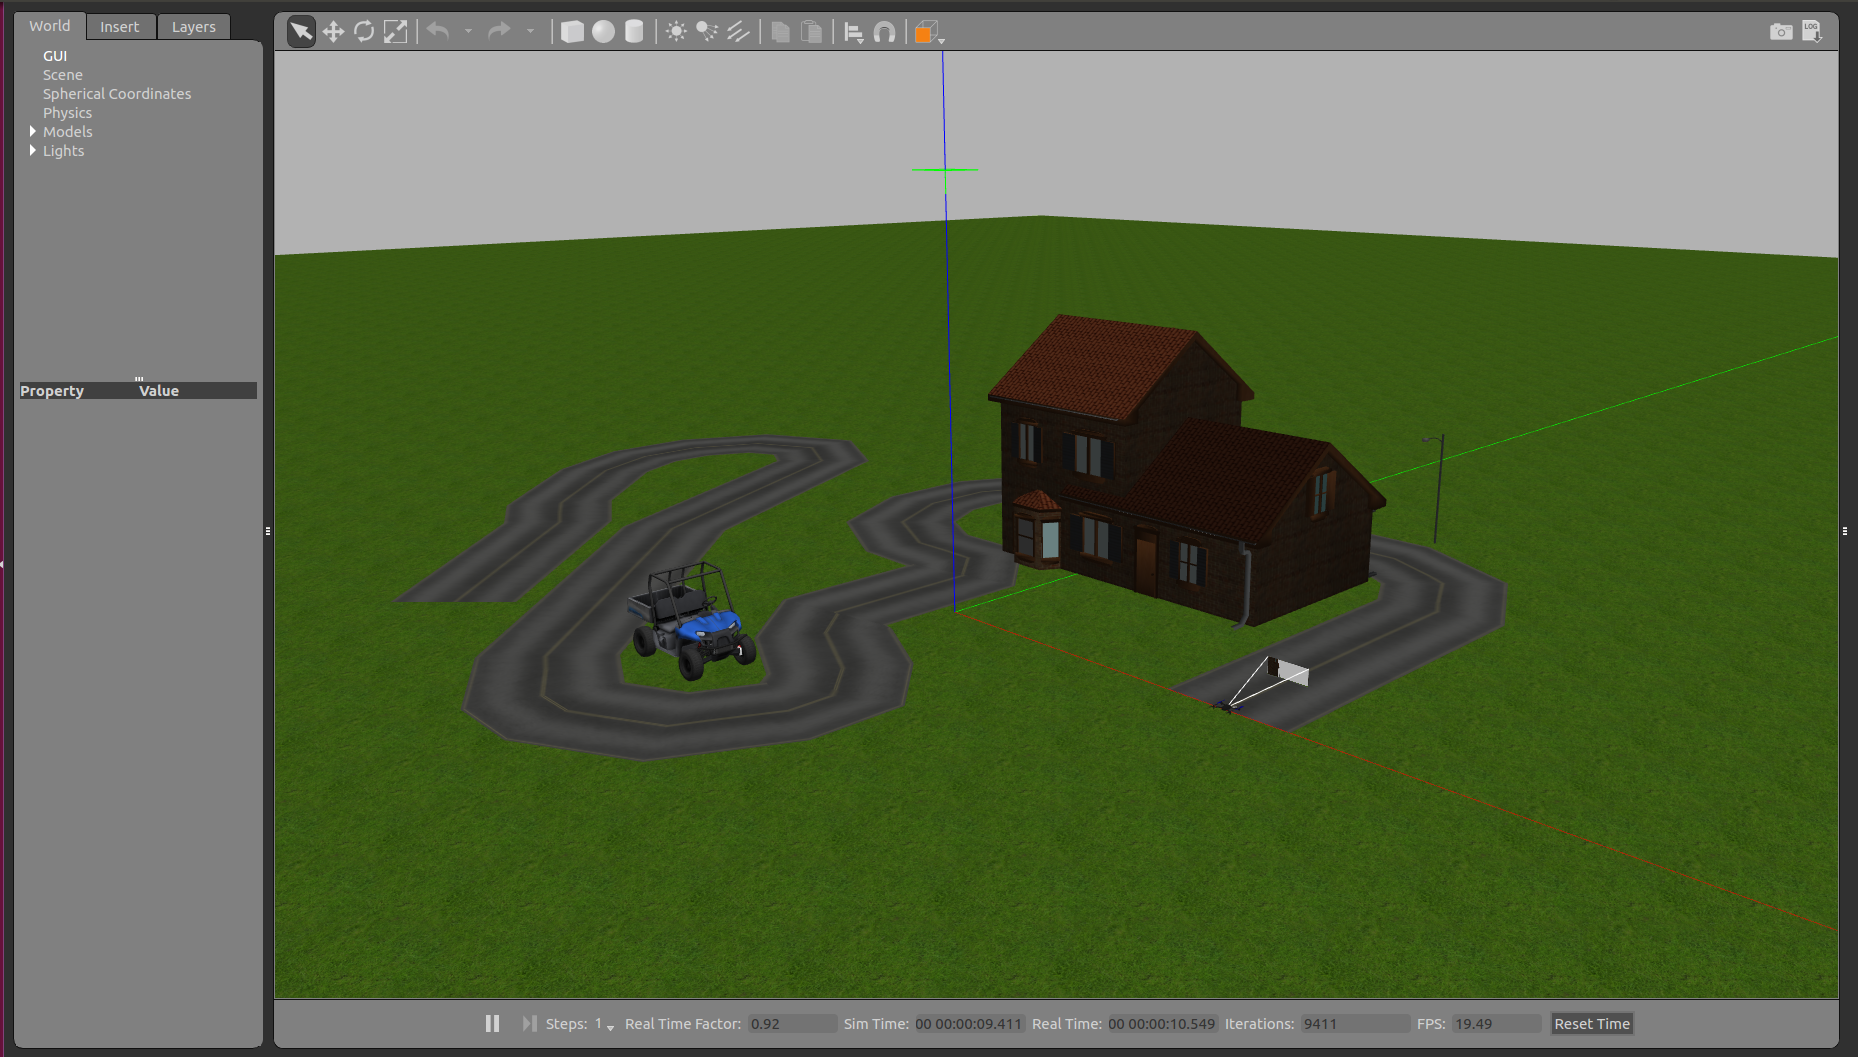
\includegraphics[width=0.98\textwidth]{figures/roslaunch_fr.png}
		\caption{Inicialización ROS y Gazebo}
		\label{fig.roslaunchfr}
		\end{center}
\end{figure}

Para iniciar el componente académico, será necesario ejecutar otro comando en una terminal distinta:

\lstset{language=bash, breaklines=true, basicstyle=\footnotesize}
\begin{lstlisting}[frame=single]
cd ~/Academy/exercises/follow\_road
python2 follow\_road.py
\end{lstlisting}

Una vez ejecutado el comando, el componente académico enlazará los sensores y actuadores proporcionados por \textit{ROS-Kinetic} mediante el fichero de configuración lanzado previamente a la variable \textit{self.drone} que contiene las variables:

\begin{itemize}
    \item self.cameraVentral
    \item self.cameraFrontal
    \item self.pose3d
    \item self.cmdvel
    \item self.extra
\end{itemize}

Con la variable \textit{self.drone}, el nodo académico se comunica con los \textit{drivers} de \textit{ROS-Kinetic}.
Además de realizar la conexión con los sensores y actuadores, al ejecutar la instrucción, nos aparecerá la interfaz gráfica de usuario (GUI) en la que se podrá visualizar las imágenes recogidas por la cámara, los botones de control y el teleoperador (Figura \ref{fig.inaGfr}).

\begin{figure}[H]
  \begin{center}
    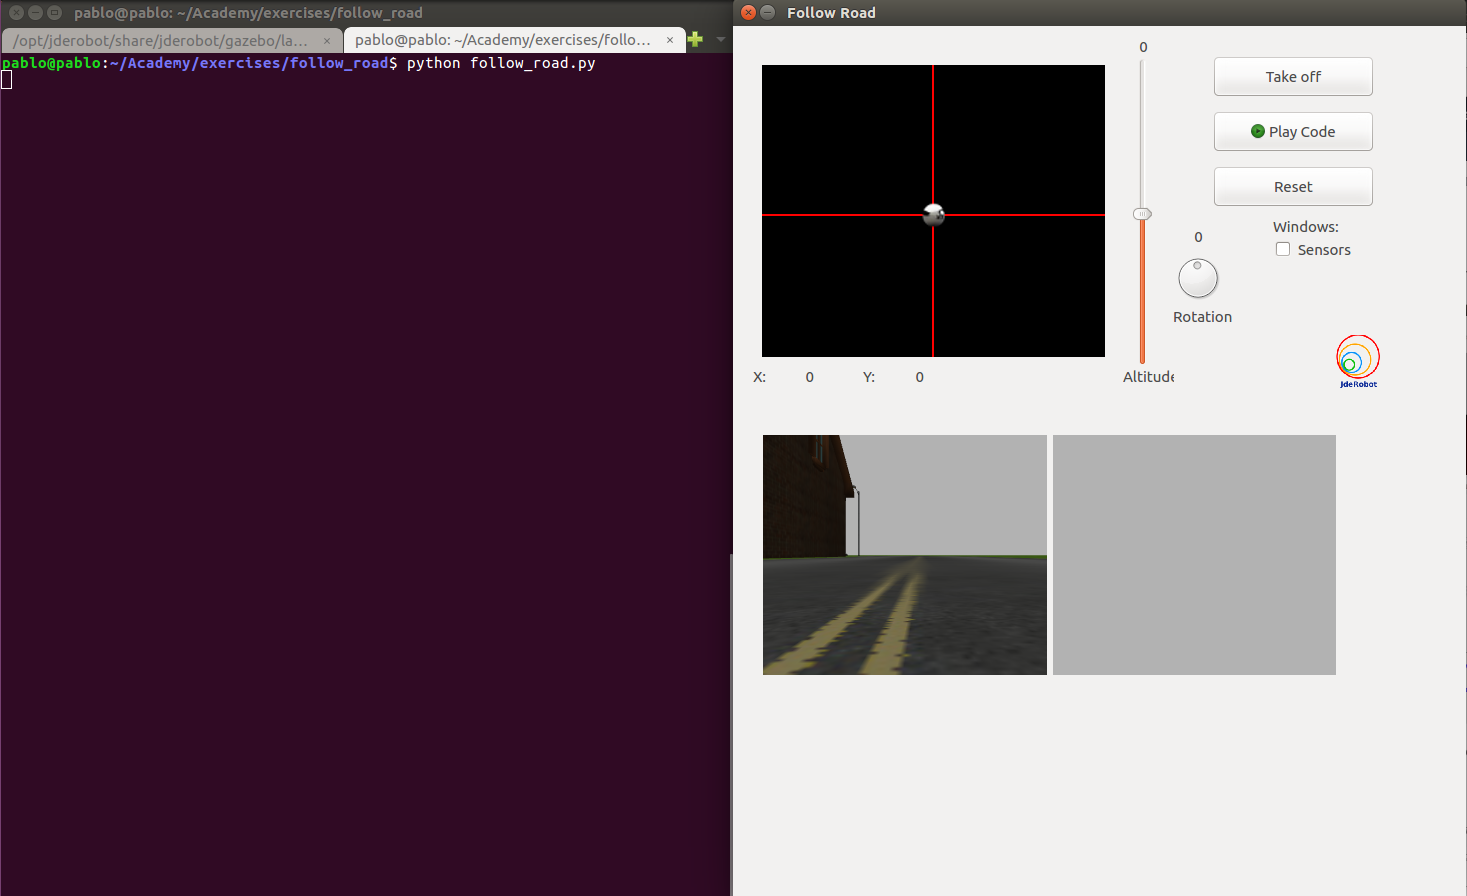
\includegraphics[width=0.98\textwidth]{figures/init_na_fr.png}
		\caption{Inicialización del nodo académico y el GUI}
		\label{fig.inaGfr}
		\end{center}
\end{figure}

Una vez inicializados los \textit{drivers de ROS-Kinetic}, el escenario en el simulador y el nodo académico, con su GUI, se puede iniciar el algoritmo desarrollado por el alumno pulsando sobre el botón ``Play Code''. De esta manera, la lógica programada podrá ser visualizada tanto en el GUI, como en el simulador.

\subsection{Ejecución estática}
En el caso en el que el alumno no programe el control de movimiento en su algoritmo, es posible ejecutar el código de igual manera. Esto es útil para depurar el algoritmo de procesamiento de imagen. 

El alumno tiene dos opciones en este aspecto. La primera consiste en dejar el robot inmóvil y ver el procesamiento realizado en la ventana para la imagen procesada del GUI. 

\begin{figure}[H]
  \begin{center}
    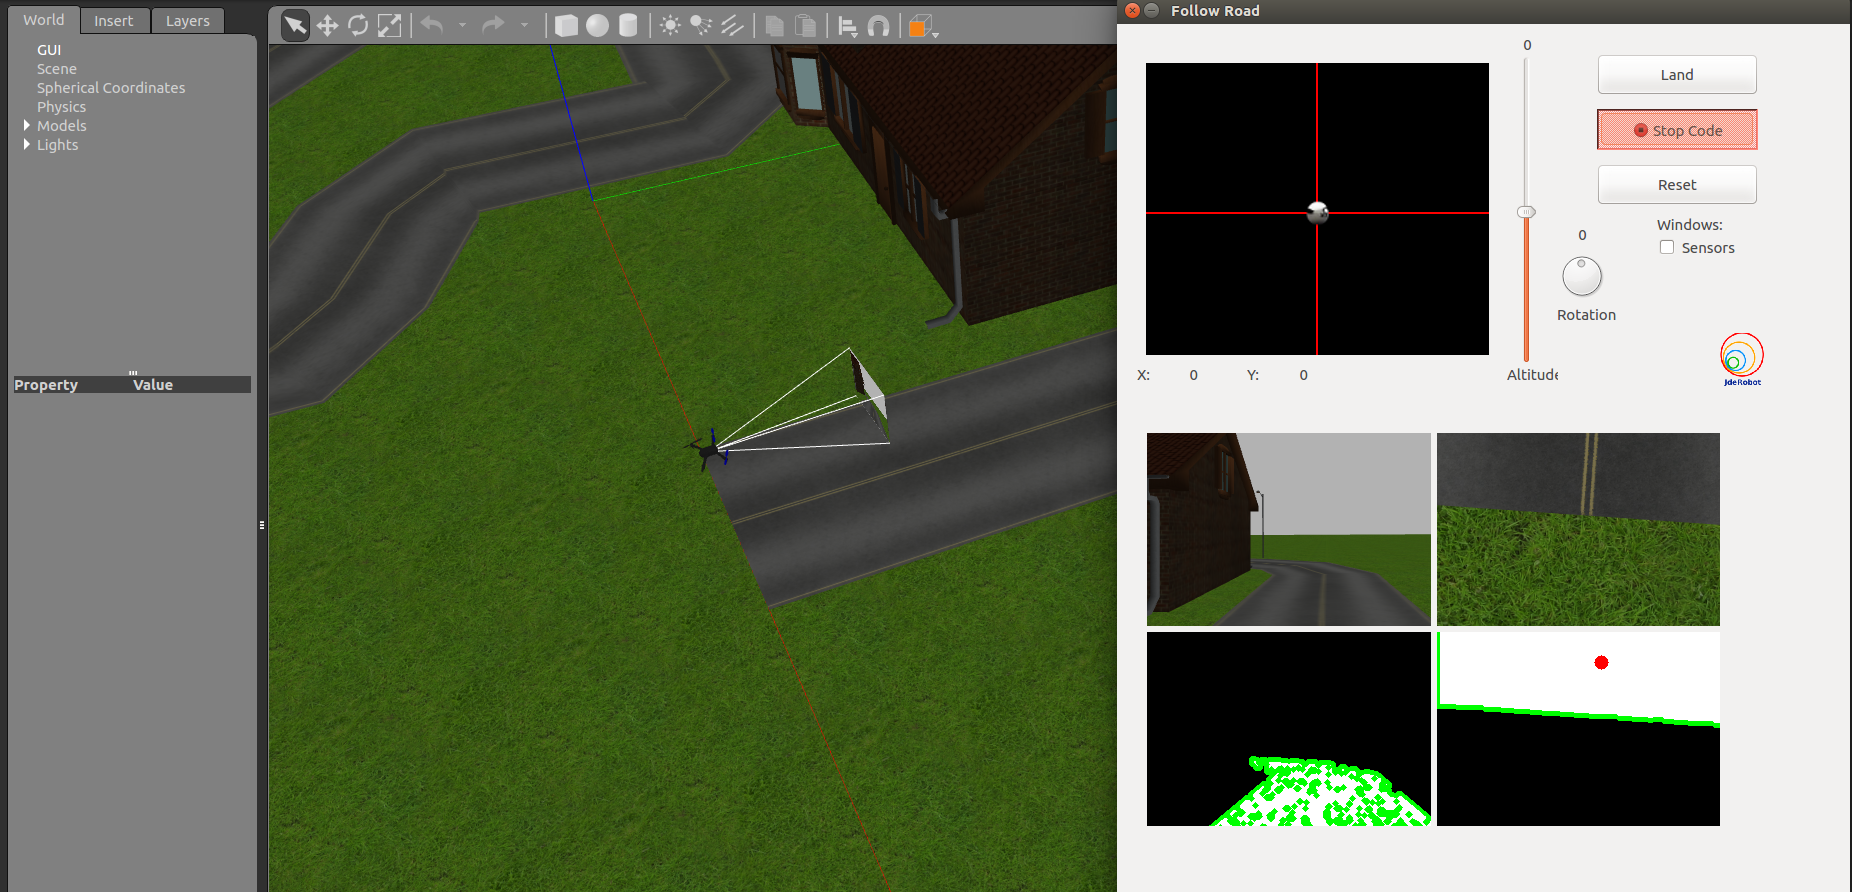
\includegraphics[width=0.98\textwidth]{figures/ejec_estat_fr.png}
		\caption{Ejecución estática de la práctica}
		\label{fig.eefr}
		\end{center}
\end{figure}

Otra opción, una vez haya superado esa primera prueba, es utilizar el teleoperador para mover el dron y visualizar el filtrado en movimiento.

\begin{figure}[H]
  \begin{center}
    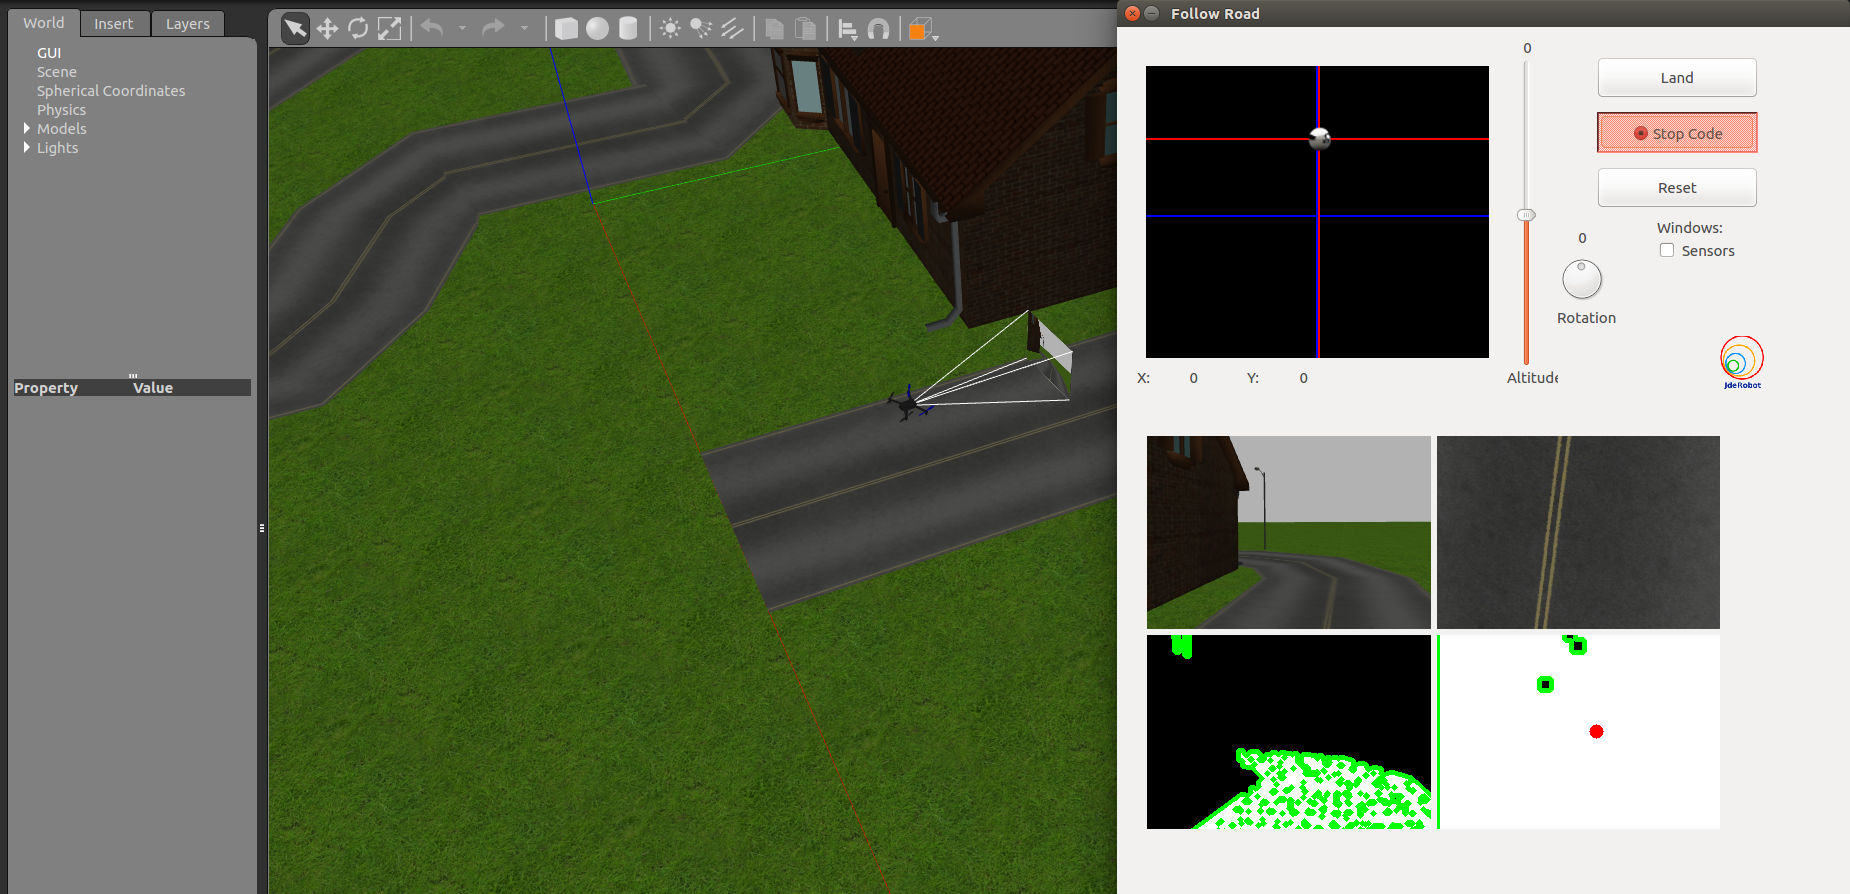
\includegraphics[width=0.98\textwidth]{figures/ejec_semiestat_fr.png}
		\caption{Ejecución con teleoperador}
		\label{fig.esefr}
		\end{center}
\end{figure}

Con esta ejecución semi-móvil de la práctica, el alumno también puede visualizar el comportamiento del robot al movimiento y el procesado dinámico de la imagen. Con esto, el alumno se puede hacer una idea de la velocidad a la que tiene que programar el control de movimiento para seguir la carretera.
\lhead[]{CAP\'ITULO \thechapter. CONCLUSIONES}
\chapter{Conclusiones}\label{cap.conclusiones}
Una vez documentadas en profundidad las dos prácticas desarrolladas en este Trabajo de Fin de Grado, se dedicará el siguiente capítulo a la comprobación de la consecución de los objetivos alcanzados, así como a la explicación de los conocimientos adquiridos y una breve exposición de posibles mejoras de las prácticas y de las líneas de actuación futuras.

\section{Conclusiones}
El objetivo principal de desarrollar una nueva práctica y la consecución de una mejora notoria en otra de las prácticas del entorno JdeRbot-Academy ha sido alcanzado con éxito. Prueba de ello son, tanto su inclusión en el programa de prácticas, como el correcto funcionamiento del nodo académico y de la solución de referencia desarrollada. Este objetivo principal estaba subdividido en objetivos secundarios de los cuales se detallará a continuación si han sido alcanzado y la manera para ello.

El primer objetivo secundario establecido fue la mejora de una práctica existente del entorno de JdeRobot-Academy. La práctica escogida fue el sigue carreteras o \textit{Follow Road}. Este objetivo se logró alcanzar dado que la práctica fue completamente optimizada y mejorada. Se desarrollaron mejoras en la interfaz gráfica y el nodo académico, como la introducción de un visor de imágenes filtradas y el desarrollo de una pausa académica. Además, se realizó una optimización de la práctica incluyendo \textit{drivers} de ROS para der un mejor soporte a su infraestructura. De esta manera se tuvo que hacer una readaptación de las conexiones del nodo académico con sensores y actuadores del robot. Después de todas estas modificaciones se consiguió una práctica totalmente operativa y actualizada. Tanto es así, que la renovación de la interfaz gráfica se incluyó en las prácticas similares del entorno JdeRobot-Academy.

El siguiente objetivo fue el desarrollo de una práctica completamente nueva llamada \textit{Chrono}. Este objetivo fue bastante complejo debido a la implementación de una reproducción sincronizada que se adapte al rendimiento de cada ordenador. Además, la práctica debe grabar la simulación actual para su posterior reproducción en el caso de que el algoritmo desarrollado sea más rápido que la grabación. Adicionalmente, otro punto de gran complejidad era la visión de la posición del F1 con el récord del circuito en la interfaz gráfica del nodo académico, punto que también se consiguió solventar. A parte de estas tareas especialmente complejas, se tuvo que desarrollar la práctica desde cero, incluyendo el nodo académico, la conexión con los sensores actuadores del robot y el fichero para albergar la solución del estudiante.

En relación con los dos objetivos anteriores, se fijaron dos objetivos nuevos, los cuales establecían el desarrollo de una solución para cada práctica. Este punto incluía el estudio de técnicas de captación, procesado y control de imágnes y control del movimiento del robot. Además, sirve de punto de referencia para el desarrollo de la solución por los estudiantes. Ambos objetivos fueron alcanzados satisfactoriamente.

Para la solución de la primera práctica fue necesario el estudio de técnicas de procesado de imágenes para realizar un filtro de partículas para filtrar la carretera del resto del escenario. Una vez realizado el primer filtro fue necesario aplicar técnicas del postprocesado de imágenes para adaptar la imagen filtrada y localizar el centro de la carretera. Además, fue necesario el estudio de movimiento del dron para poder realizar un movimiento controlado. Este movimiento es muy sensible debido al control de la actitud y la inclinación del dron que pueden afectar a la visualización de las imágenes captadas por la cámara.

Para la solución de la segunda práctica se tuvo que realizar un estudio paralelo de filtrado y postprocesado de imagen para captar y procesar las imágenes grabadas por la cámara del coche. Además de adquirir los conocimientos de movimiento para el robot F1 utilizando los \textit{drivers} de ROS. Es importante destacar que en este caso se tuvo que realizar una solución más rápida que el algoritmo con el récord del circuito optimizado a partir de una solución previa. Es decir, en este caso se tuvieron que realizar dos soluciones distintas, una optimizada y otra desde cero.

Tras la consecución de los objetivos anteriores, se realizó una readaptación de las prácticas para su inclusión en la plataforma web Jupyter. De esta manera el estudiante dispondrá de las mismas prácticas que las disponibles en el entorno JdeRobot pero con cuadernillos en lugar de nodo académico. De esta manera, el nodo académico es transparente al alumno, que dispone de una celda para desarrollar su algoritmo y solo tendrá que ejecutar dicha celda para ver su estado.
Para lograr dicho objetivo fue necesario adquirir conocimientos de Jupyter así como un estudio de nuevos procesos de Python.

El siguiente objetivo respecto a la primera práctica fue su inclusión en el entorno docente JdeRobot-Academy-Web. De esta manera se da un paso más hacia un soporte multiplataforma. Esto es debido a que Academy-Web utiliza Dockers para ejecutar las prácticas en el navegador. Para poder alcanzar este objetivo hubo que estudiar el entorno JdeRobot-AcademyWeb, y el estudio de Dockers, campos totalmente desconocidos.

Por último, gracias a una motivación personal, se ha conseguido adquirir conocimientos para afrontar problemas reales de ingeniería que comprenden tanto software como hardware. Debido a esto se ha adquirido experiencia para integrarse en proyectos de robótica, desde su infraestructura, las conexiones hardware-software, las interfaces, componentes, funcionalidad, así como la part visible al usuario. También se han adquiridos conocimientos de simulación, y diseño gráfico, así como herramientas de tratamiento de imagen y técnicas de programación.

\section{Trabajos futuros} 
El presente Trabajo de Fin de Grado ha expuesto una nueva vía para la realización de proyectos en el futuro.

En la práctica del dron que ha de seguir una carretera, se expone la posibilidad de realizar un \textit{TeleTaxi}, es decir, un dron con inteligencia parecida a la de esa misma práctica. De esta manera podría realizarse una práctica en la que, con un mapa previo, se le indique al dron al punto al que debe dirigirse en un plano de ciudad. De esta manera se podría dotar al dron de la inteligencia necesaria para ser un "Dron repartidor".

Respecto a la práctica de \textit{Chrono}, sería interesante el desarrollo de una competición en distintos circuitos y la inclusión de distintos coches, cada uno con su propio algoritmo, que compitan entre ellos para conocer el algoritmo más eficiente en cada circuito. De esta manera se estaría desarrollando un Grand Pix de robots F1.

Otro punto de desarrollo futuro sería la realización de nuevos algoritmos que permitan un rendimiento más eficiente y rápido a los propuestos en este Trabajo de Fin de Grado.

%%%%%%%%%%%%%%% Bibliogra��a %%%%%%%%%%%%%%%

\nocite{*}
\lhead[]{BIBLIOGRAF\'IA}
\bibliographystyle{acm}
\bibliography{bibliografia}
\addcontentsline{toc}{chapter}{Bibliografía}
\end{document}